\documentclass[10pt, landscape]{article}
\usepackage[scaled=0.92]{helvet}
\usepackage{calc}
\usepackage{multicol}
\usepackage[a4paper,margin=3mm,landscape]{geometry}
\usepackage{amsmath,amsthm,amsfonts,amssymb}
\usepackage{color,graphicx,overpic}
\usepackage{hyperref}
\usepackage{newtxtext} 
\usepackage{enumitem}
\usepackage[table]{xcolor}
\usepackage{mathtools}
\setlist{nosep}
% for including images
\graphicspath{ {./images/} }

\pdfinfo{
  /Title (CS4231.pdf)
  /Creator (TeX)
  /Producer (pdfTeX 1.40.0)
  /Author (Jovyn Tan)
  /Subject (CS4231)
/Keywords (CS4231, nus,cheatsheet,pdf)}

% Turn off header and footer
\pagestyle{empty}

% redefine section commands to use less space
\makeatletter
\renewcommand{\section}{\@startsection{section}{1}{0mm}%
  {-1ex plus -.5ex minus -.2ex}%
  {0.5ex plus .2ex}%x
{\normalfont\large\bfseries}}
\renewcommand{\subsection}{\@startsection{subsection}{2}{0mm}%
  {-1explus -.5ex minus -.2ex}%
  {0.5ex plus .2ex}%
{\normalfont\normalsize\bfseries}}
\renewcommand{\subsubsection}{\@startsection{subsubsection}{3}{0mm}%
  {-1ex plus -.5ex minus -.2ex}%
  {1ex plus .2ex}%
{\normalfont\small\bfseries}}%
\makeatother

\renewcommand{\familydefault}{\sfdefault}
\renewcommand\rmdefault{\sfdefault}
%  makes nested numbering (e.g. 1.1.1, 1.1.2, etc)
\renewcommand{\labelenumii}{\theenumii}
\renewcommand{\theenumii}{\theenumi.\arabic{enumii}.}
\renewcommand\labelitemii{•}
\renewcommand\labelitemiii{•}

\definecolor{mathblue}{cmyk}{1,.72,0,.38}
\everymath\expandafter{\the\everymath \color{mathblue}}

% Don't print section numbers
\setcounter{secnumdepth}{0}

\setlength{\parindent}{0pt}
\setlength{\parskip}{0pt plus 0.5ex}
%% adjust spacing for all itemize/enumerate
\setlength{\leftmargini}{0.5cm}
\setlength{\leftmarginii}{0.5cm}
\setlist[itemize,1]{leftmargin=2mm,labelindent=1mm,labelsep=1mm}
\setlist[itemize,2]{leftmargin=4mm,labelindent=1mm,labelsep=1mm}
\setlist[itemize,3]{leftmargin=4mm,labelindent=1mm,labelsep=1mm}

% adding my commands
% tightcenter
\newenvironment{tightcenter}{%
  \setlength\topsep{0pt}
  \setlength\parskip{0pt}
  \begin{center}
    }{%
  \end{center}
}

% boxed
\newenvironment{tightbox}{%
  \setlength\topsep{0pt}
  \setlength\parskip{0pt}
  \begin{center}
    \begin{tabular}{|@{\hspace{\dimexpr\fboxsep+0.5\arrayrulewidth}}c@{\hspace{\dimexpr\fboxsep+0.5\arrayrulewidth}}|}
      \hline
    }
    {%
    \\ \hline
    \end{tabular}
  \end{center}
}

% fixed width box
\newenvironment{fixedbox}[1][0.7]{
  \setlength\topsep{0pt}
  \setlength\parskip{0pt}
  \begin{center}
    \begin{tabular}{|>{\centering\arraybackslash}m{#1\linewidth}|}
    \hline
  }{
  \\ \hline
  \end{tabular}
  \end{center}
}

% definition of a new term
\usepackage{soul}
\definecolor{paleyellow}{RGB}{251,243,218}
\newcommand{\definition}[2][]{\sethlcolor{paleyellow}\hl{\textbf{#2}} #1  $\rightarrow$}
% inline definition
\newcommand{\ildefinition}[1]{\sethlcolor{paleyellow}\hl{\textbf{#1}}}

% important note (attention)
\newcommand{\attention}{{\color{red}\textbf{! }}}

% nice proof
\newenvironment{niceproof}[1][Proof]
{%
  \sbox0{\textit{#1}. }%
  \list{}{\labelwidth\wd0 \leftmargin\wd0 \labelsep 0pt }
\item[\usebox0]}
  {\endlist}


\usepackage{color, soul}
\usepackage{listings}
\usepackage{inconsolata}

\definecolor{codegreen}{rgb}{0,0.6,0}
\definecolor{codegray}{rgb}{0.5,0.5,0.5}
\definecolor{codepurple}{HTML}{C42043}
\definecolor{backcolour}{HTML}{F2F2F2}
\definecolor{bookColor}{cmyk}{0,0,0,0.90}

\newcommand{\code}[1]{\texttt{\sethlcolor{backcolour}\hl{$\,$#1$\,$}}}

% SQL code blocks
% define SQL styles
\lstdefinestyle{mySQL}{%
  language=SQL,
  backgroundcolor=\color{backcolour},
  commentstyle=\color{codegreen},
  keywordstyle=\color{codepurple},
  numberstyle=\numberstyle,
  stringstyle=\color{codepurple},
  basicstyle=\scriptsize\ttfamily,
  breaklines=true,
}

\DeclareMathOperator{\pairwisemax}{pairwise-max}

% -----------------------------------------------------------------------

\begin{document}
\raggedright
\footnotesize
\begin{multicols*}{3}
  % multicol parameters
  \setlength{\columnseprule}{0.25pt}

  \begin{center}
    \fbox{%
      \parbox{0.8\linewidth}{\centering \textcolor{black}{
          {\Large\textbf{CS4231}}
        \\ \normalsize{AY22/23 SEM 2}}
        \\ {\footnotesize \textcolor{gray}{github/jovyntls}}
      }%
    }
  \end{center}

  \section{01. MUTUAL EXCLUSION}

  \subsection{properties of a mutex algorithm}

  \begin{itemize}
    \item \definition{mutual exclusion} no more than one process in the critical section
    \item \definition{progress} if one or more process wants to enter and if no one is in the critical section, then one of them can eventually enter the critical section
    \item \definition{no starvation} if a process wants to enter, it eventually can always enter
      \begin{itemize}
        \item no starvation implies progress!
      \end{itemize}
    \item \attention if a process is in the CS, we always assume that it will eventually exit the CS
      \begin{itemize}
        \item finite number of instructions in the CS
      \end{itemize}
  \end{itemize}

  \subsection{Peterson's Algorithm}

  \begin{tightcenter}
    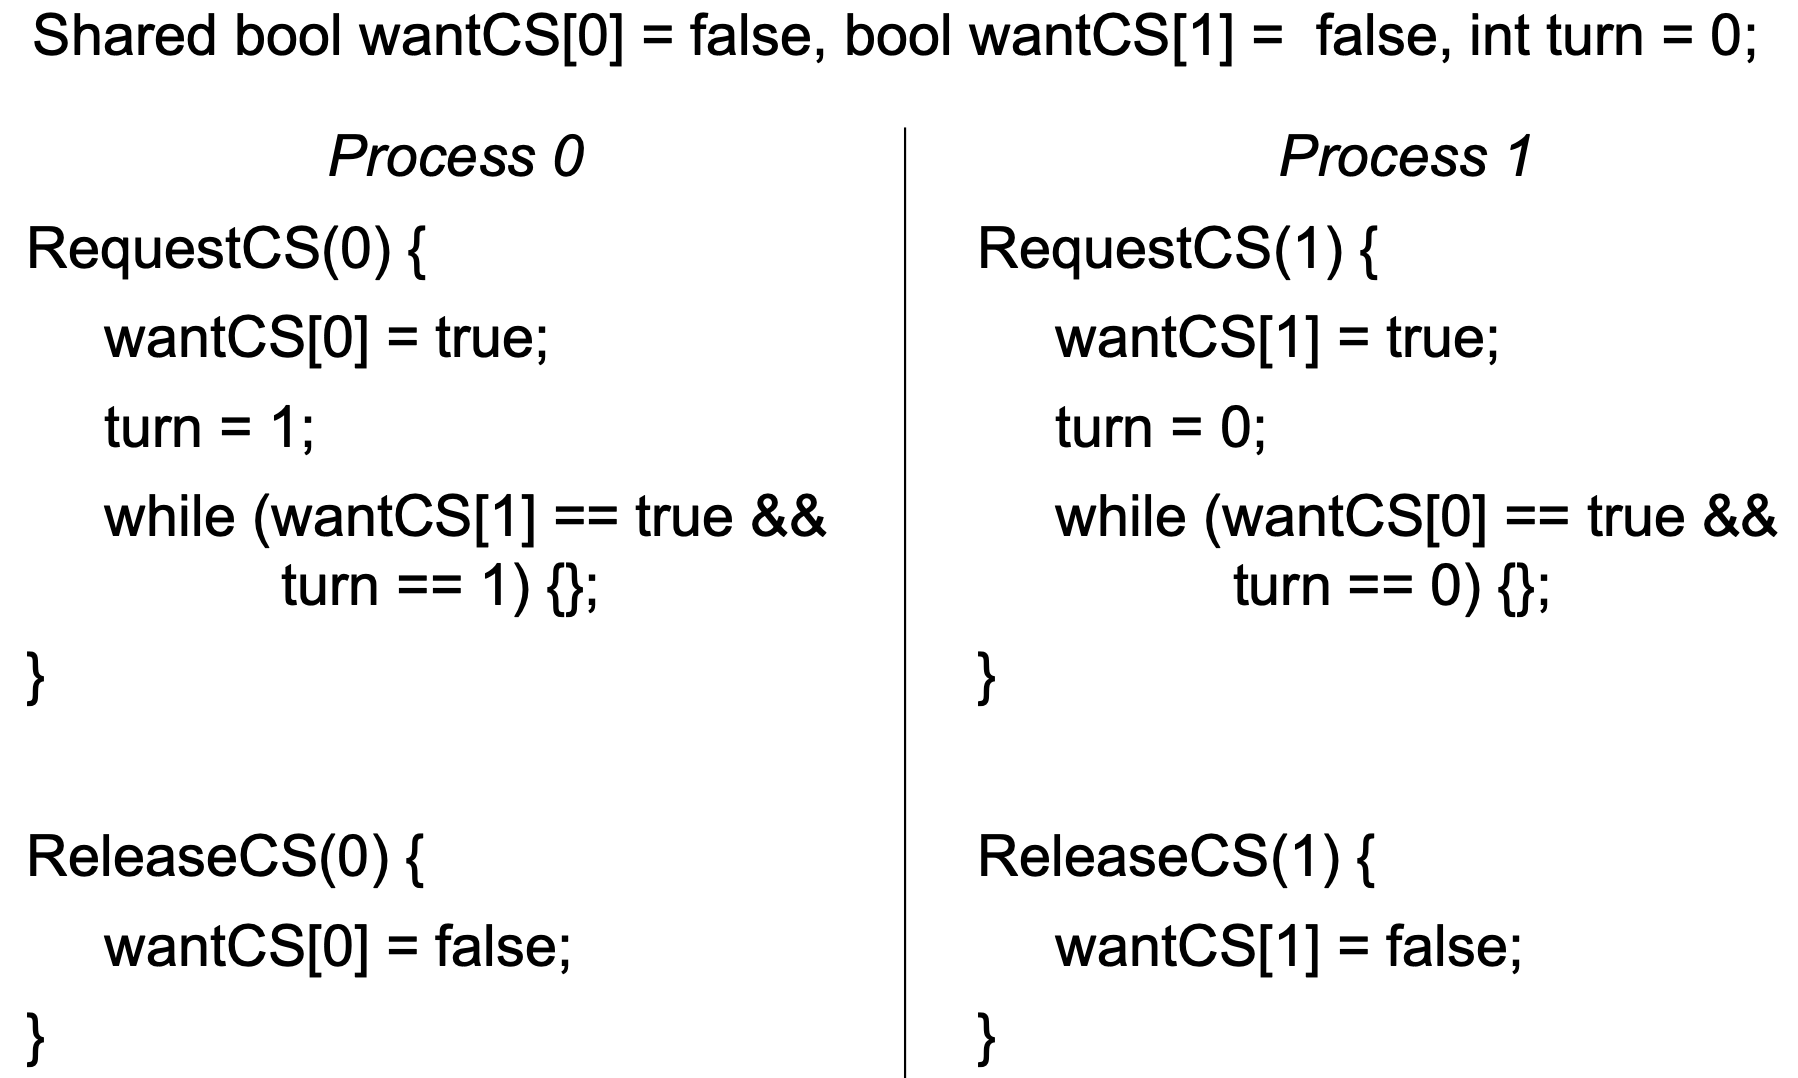
\includegraphics[width=0.7\linewidth]{cs4231-petersons-algo.png} 
  \end{tightcenter}

  \subsubsection{proof}

  \begin{itemize}
    \item \textbf{mutual exclusion}: proof by contradiction
      \begin{itemize}
        \item case 1 - turn == 0 when P0 and P1 are both in CS
          \begin{itemize}
            \item then P0 executed turn=1 before P1 executed turn=0
            \item hence wantCS[0]==false as seen by P1
            \item but wantCS[0] set to true by P0
          \end{itemize}
        \item case 2 - turn ==1. symmetric
      \end{itemize}
    \item \textbf{progress}: proof by contradiction
      \begin{itemize}
        \item suppose both want to enter but none can enter $\Rightarrow$ wantCS must be true for both
        \item case 1: turn==0. then P0 can enter
        \item case 2: symmetric
      \end{itemize}
    \item \textbf{no starvation}: proof by contradiction
      \begin{itemize}
        \item case 1: P0 is waiting, then wantCS[1]==true and turn=1
          \begin{itemize}
            \item P1 in critical region - eventually it exits and sets wantCS[1] to false
            \item (what if P1 wants to enter again immediately? then P1 will wait first because wantCS[0]==true and it has set turn==0)
          \end{itemize}
        \item case 2: P1 is waiting. symmetric
      \end{itemize}
  \end{itemize}

  \vfill\null
  \columnbreak

  \subsection{Lamport's Bakery Algorithm}

  \begin{itemize}
    \item for $n$ processes
      \begin{itemize}
        \item get a number first (weak guarantee)
        \item get served when all lower numbers have been served (sufficient for mutex)
      \end{itemize}
    \item 2 shared arrays of $n$ elements
      \begin{itemize}
        \item \texttt{boolean choosing[i] = false} $\quad\Rightarrow$ is process $i$ trying to get a number
        \item \texttt{int number[i] = 0} $\quad \Rightarrow$ the number gotten by process $i$
          \begin{itemize}
            \item number[i] > 0: process wants to enter CS and that is the queue number
          \end{itemize}
      \end{itemize}
  \end{itemize}

  \begin{tightcenter}
    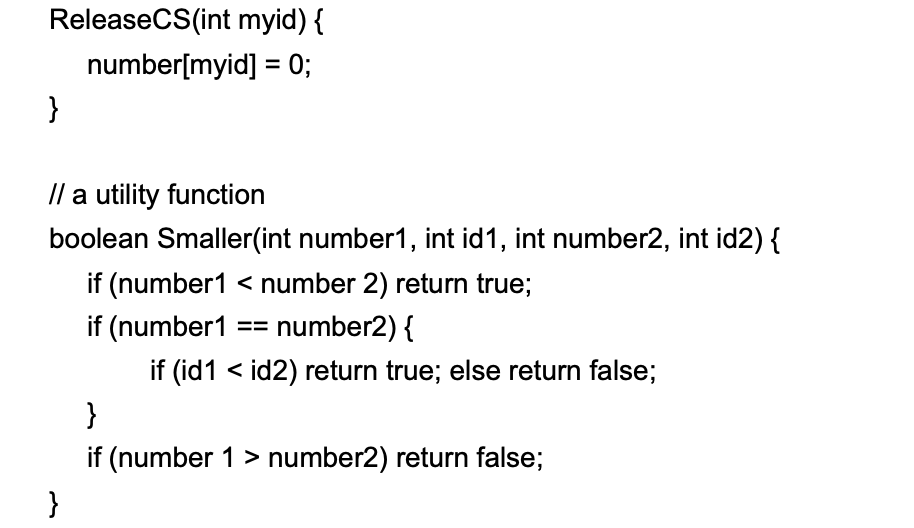
\includegraphics[width=0.7\linewidth]{cs4231-lamport-algo-release.png} 
    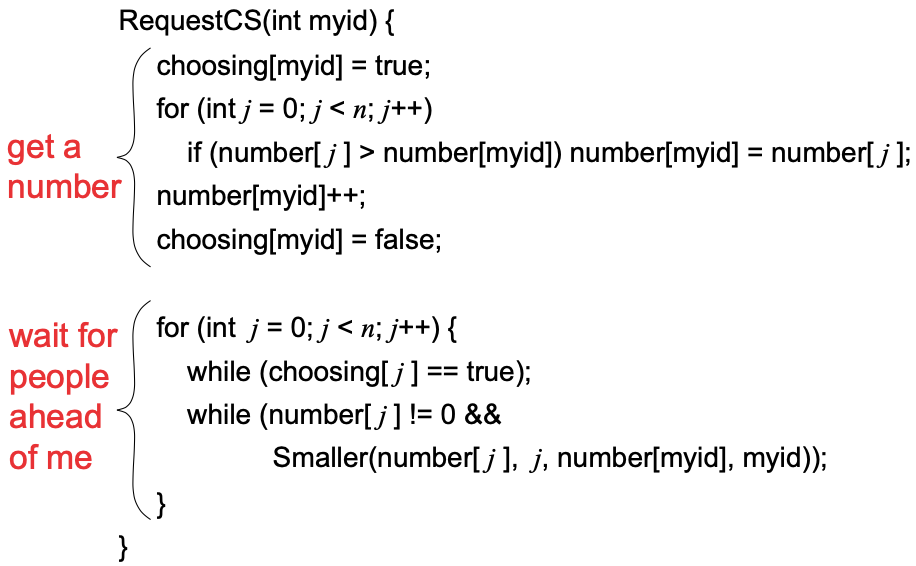
\includegraphics[width=0.7\linewidth]{cs4231-lamport-algo-request.png} 
  \end{tightcenter}

  \subsection{Hardware Solutions}

  \begin{itemize}
    \item \textbf{disable interrupts} - to prevent context switch
      \begin{itemize}
        \item do not allow context switch in the critical section
      \end{itemize}
    \item special machine-level instructions: \textbf{\texttt{TestAndSet}} executed atomically
      \begin{itemize}
        \item $\times$ when you design CPU, you want all instructions to roughly be the same complexity so that your pipelines don’t have bubbles in it
        \item $\times$ degrades performance
      \end{itemize}
  \end{itemize}

  \begin{tightcenter}
    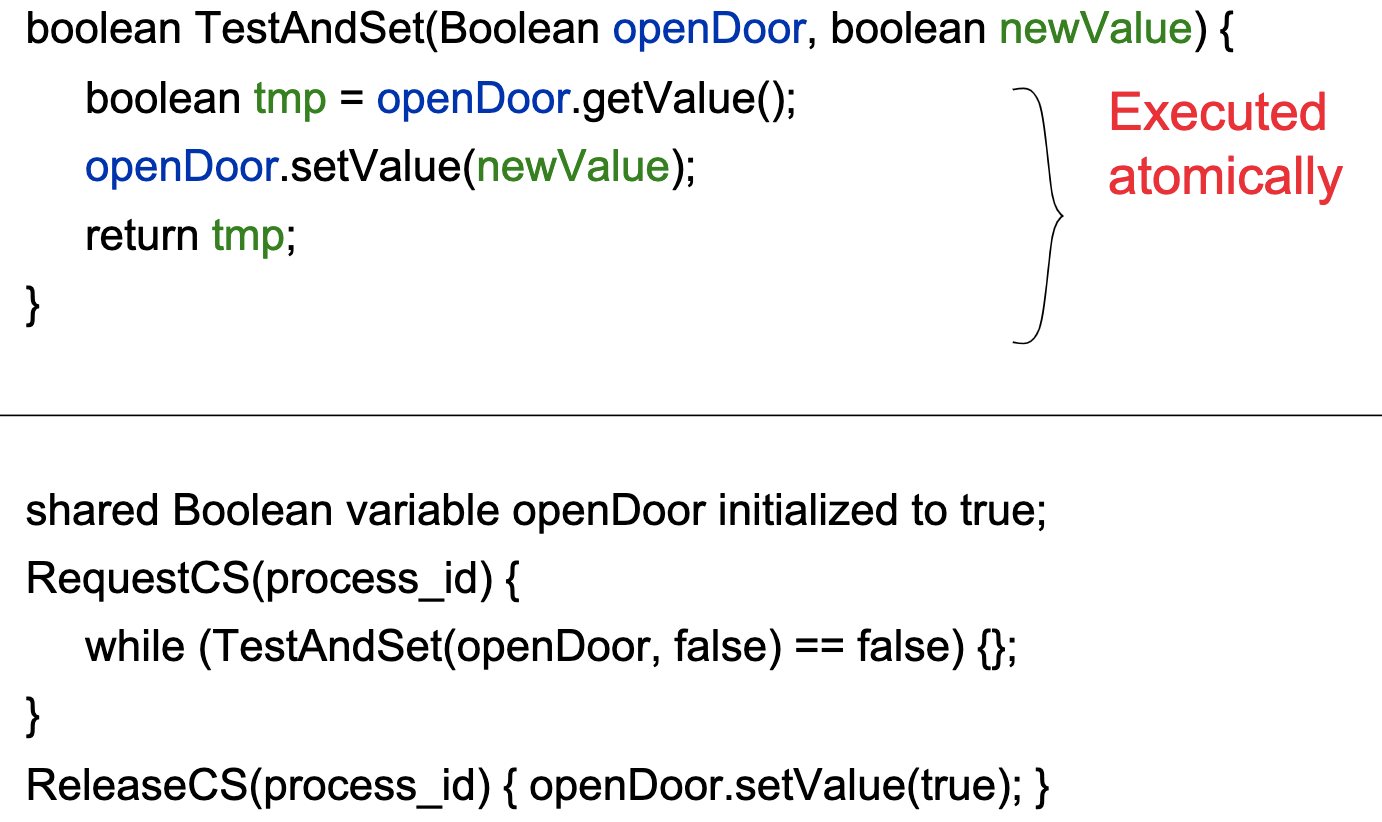
\includegraphics[width=0.7\linewidth]{cs4231-testandset.png} 
  \end{tightcenter}

  \vfill\null
  \columnbreak

  \subsection{Proof: Lamport's Bakery Algorithm}

  \begin{tightcenter}
    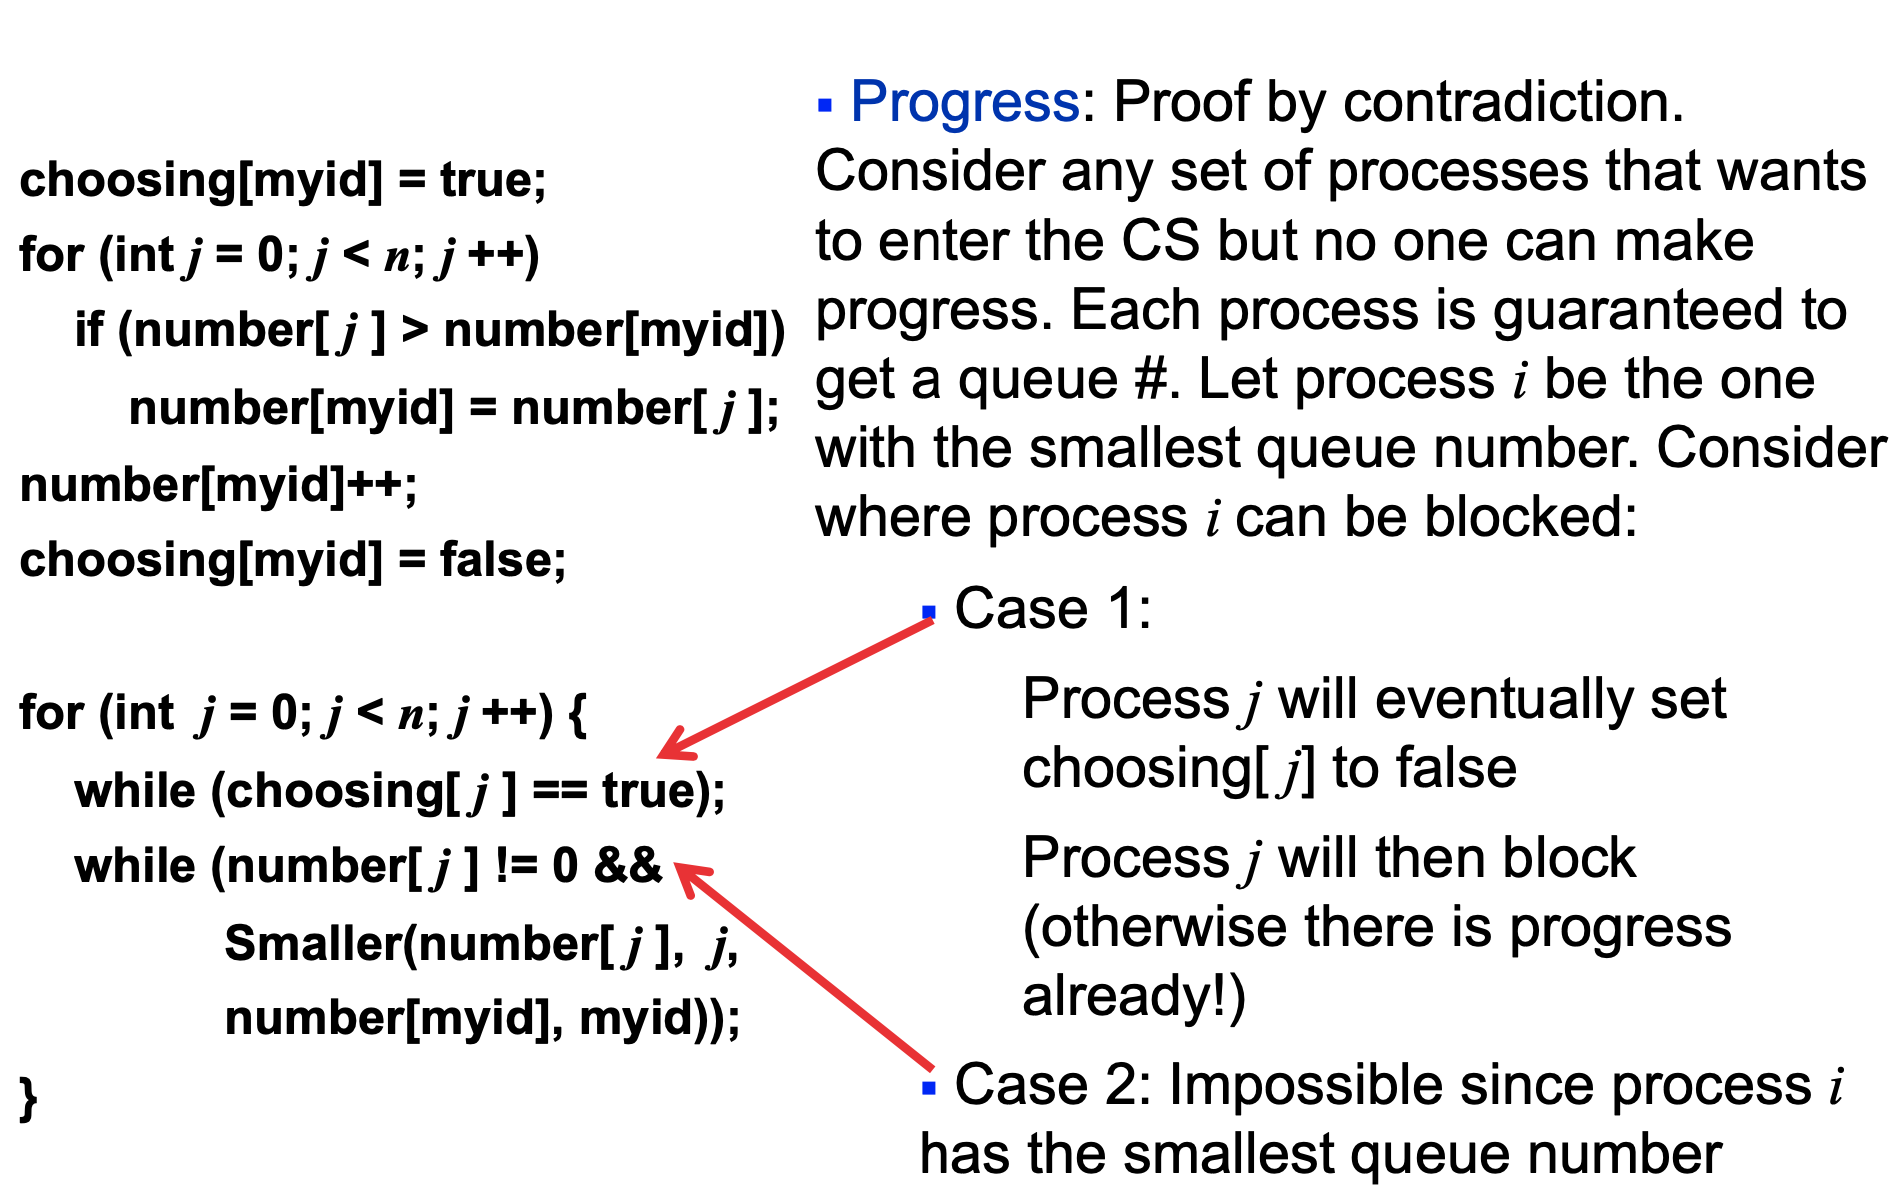
\includegraphics[width=0.95\linewidth]{cs4231-lamports-bakery-proof-1.png} 
    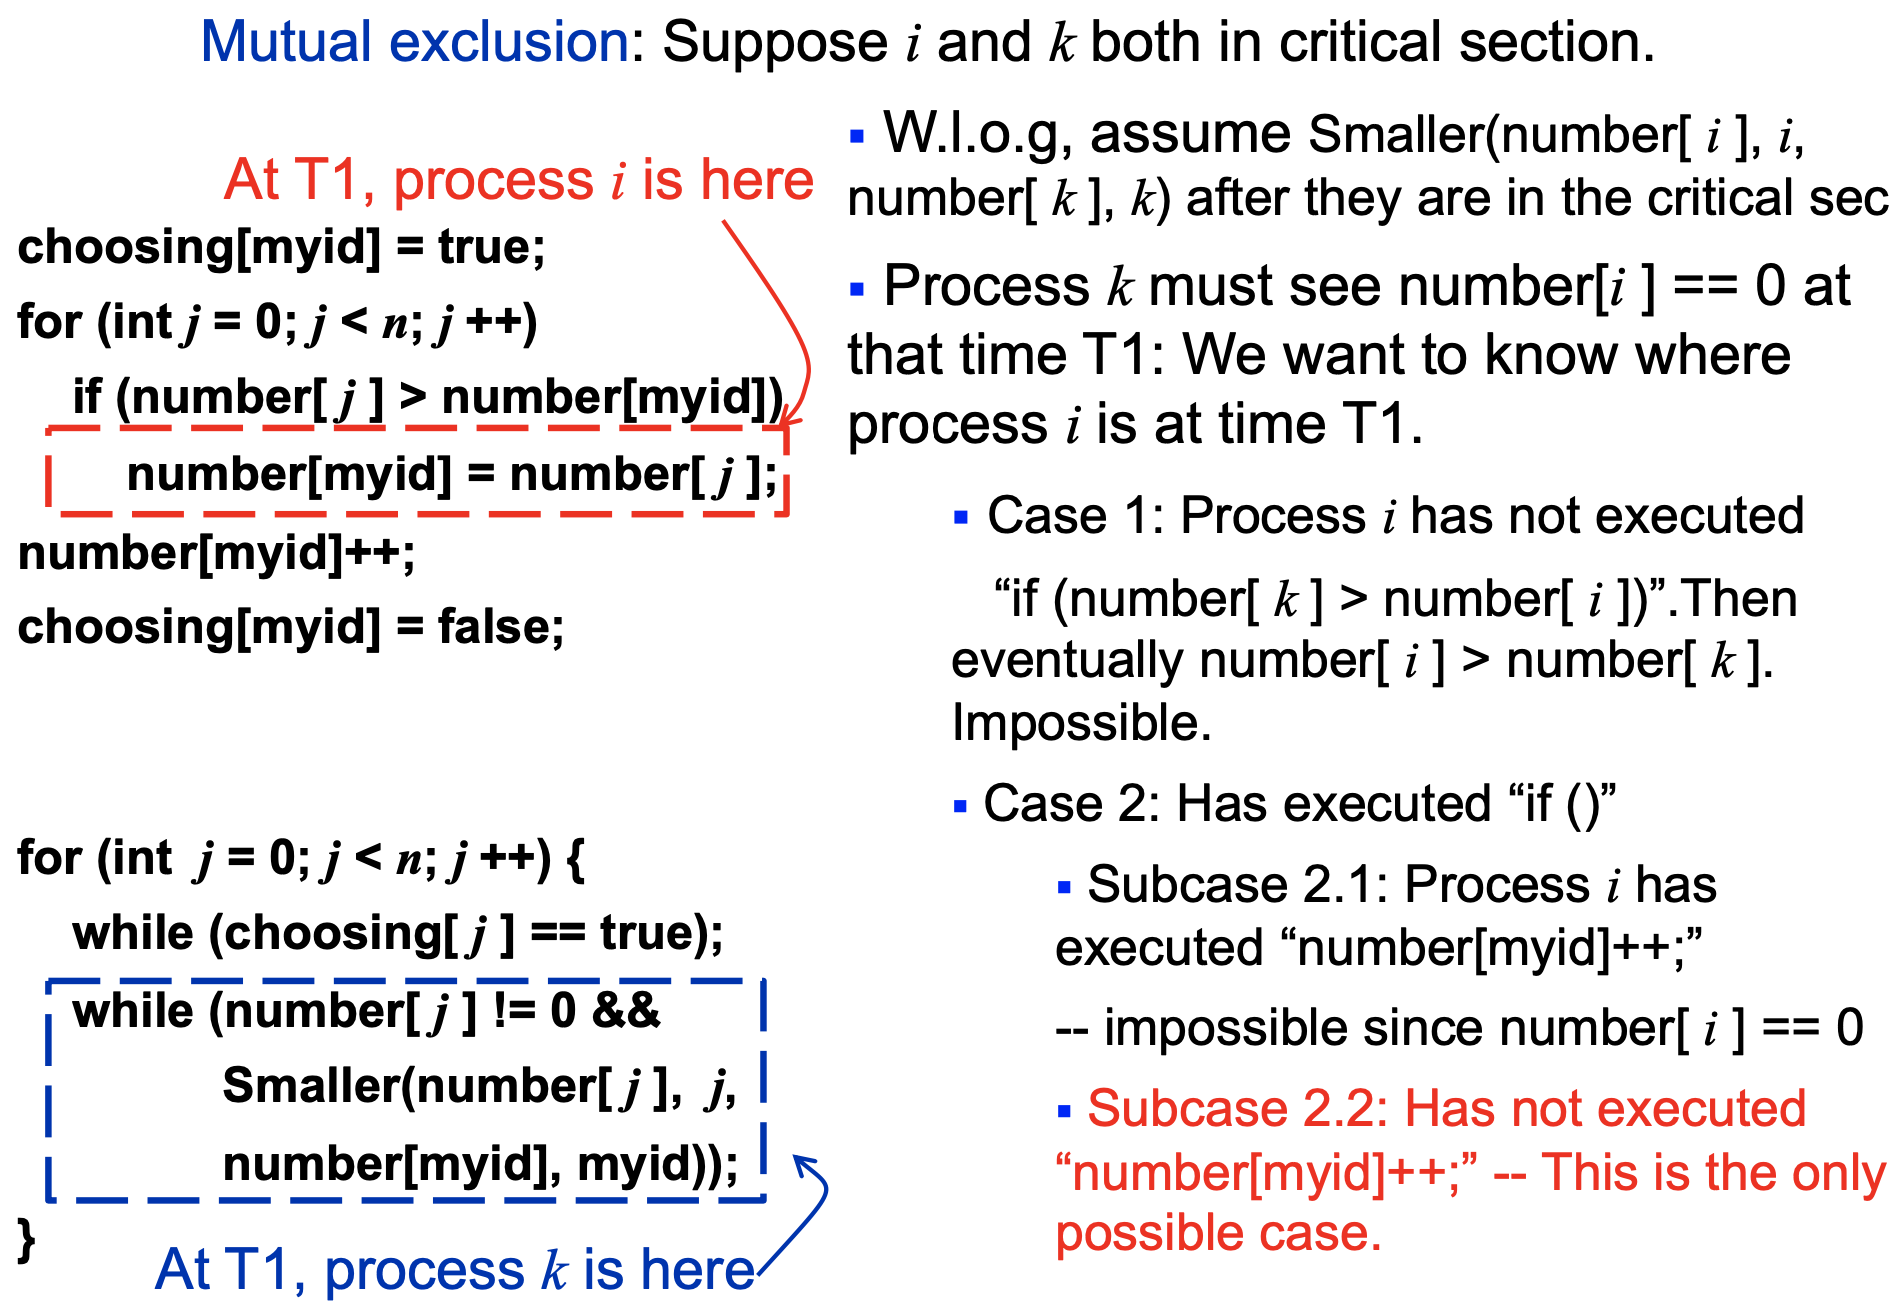
\includegraphics[width=0.95\linewidth]{cs4231-lamports-bakery-proof-2.png} 
    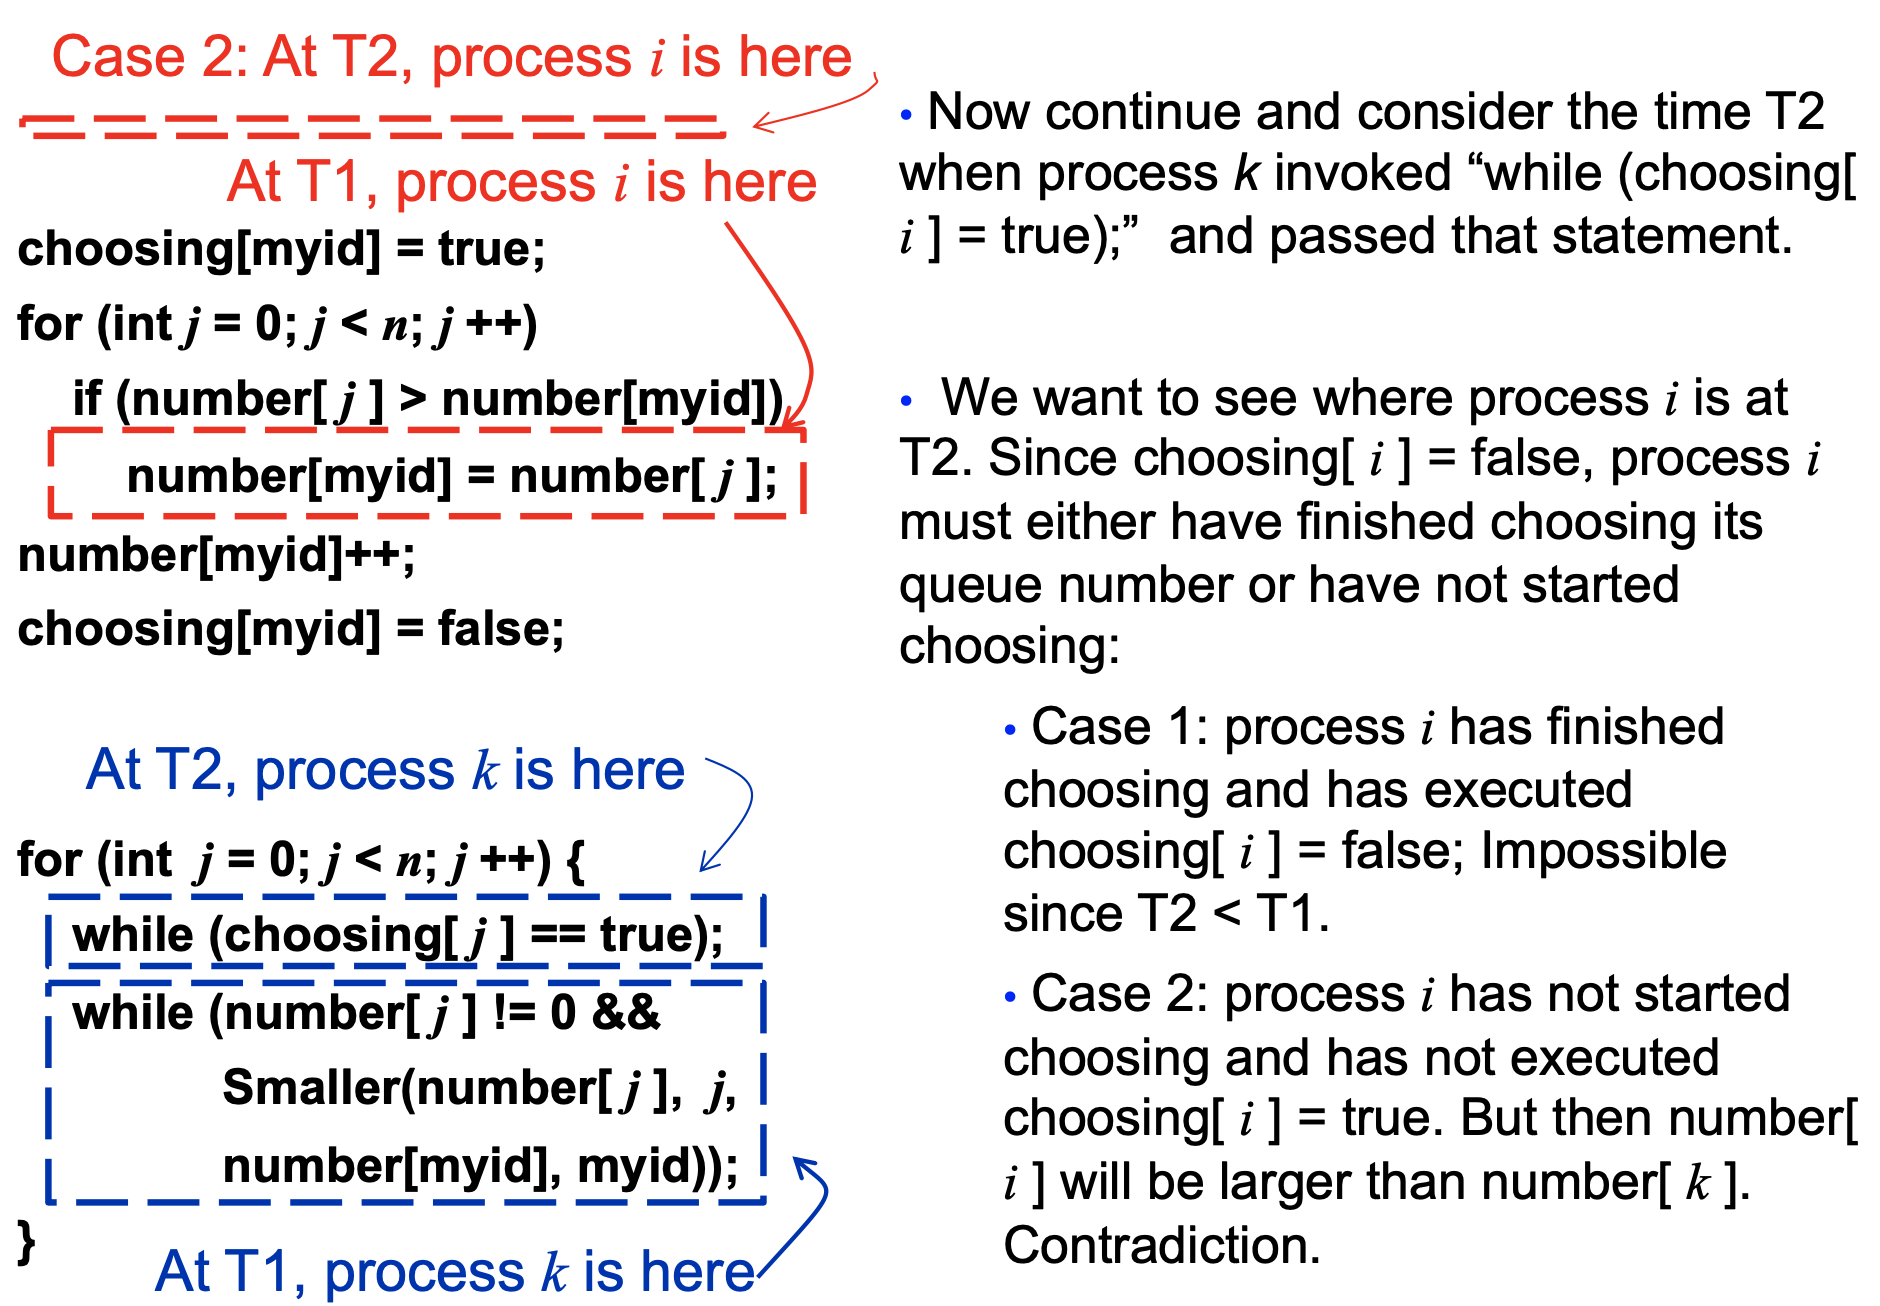
\includegraphics[width=0.95\linewidth]{cs4231-lamports-bakery-proof-3.png} 
  \end{tightcenter}

  \vfill\null
  \columnbreak

  \section{02. SYNCHRONISATION PRIMITIVES}

  \begin{itemize}
    \item solves \textbf{busy wait problem} (wastes CPU cycles)
    \item synchronisation primitives: OS-level APIs that the program may call
  \end{itemize}

  \subsection{Semaphores}

  \begin{minipage}[c]{0.55\linewidth}\color{black}      
    \textbf{2 variables} for each semaphore

    \begin{itemize}
      \item \texttt{boolean value := true}
      \item \texttt{queue} (of blocked processes) \texttt{:= empty}
    \end{itemize}

    \textbf{2 APIs, executed atomically}

    \textbf{\code{P()}} - wait
    \begin{itemize}
      \item if value == false, add self to queue and block
      \item can context switch to some other process
    \end{itemize}

    \textbf{\code{V()}} - signal
    \begin{itemize}
      \item set \texttt{value = true}
      \item wake up one arbitrary process in queue
    \end{itemize}

    \textbf{semaphore for mutex:}
    \begin{itemize}
      \item \code{RequestCS() \{ P(); \}}
      \item \code{ReleaseCS() \{ V(); \}}
    \end{itemize}
  \end{minipage}
  \begin{minipage}[c]{0.42\linewidth}
    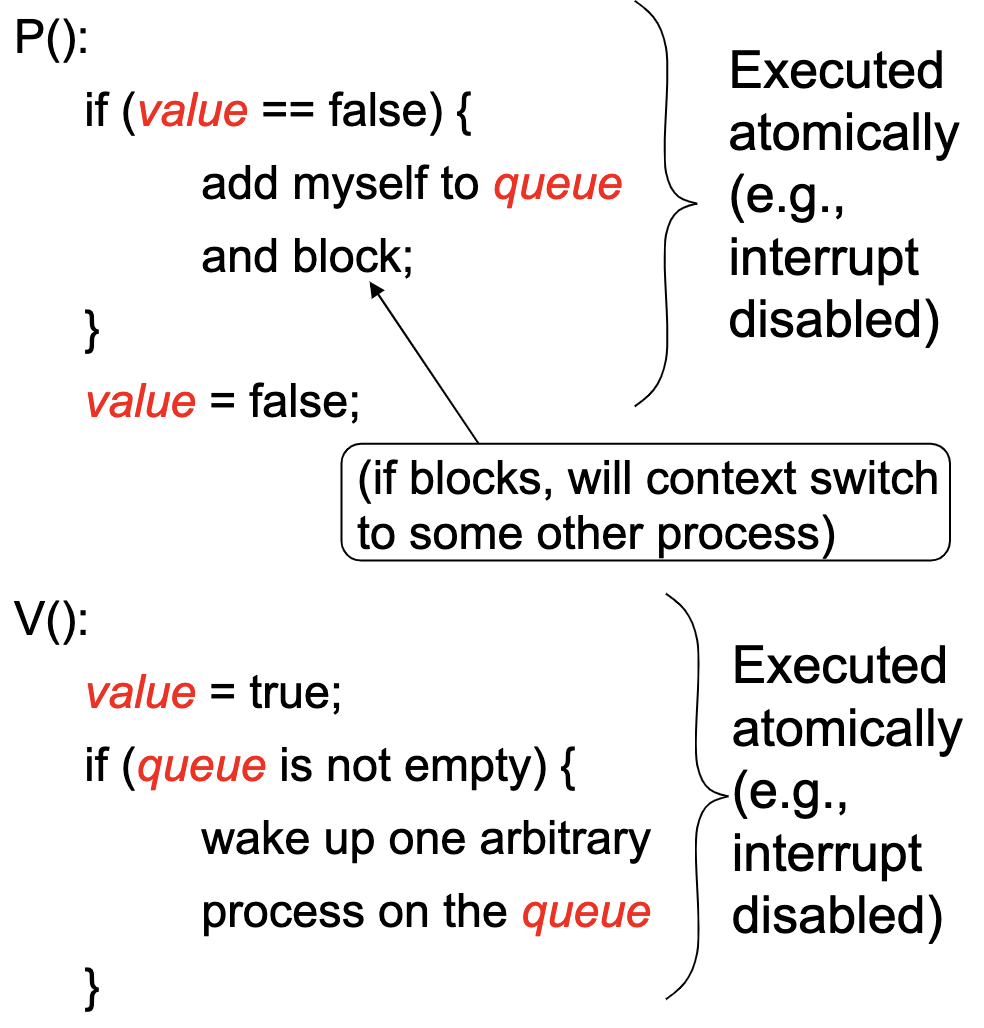
\includegraphics[width=\linewidth]{cs4231-semaphore-p-v.png} 
  \end{minipage}

  \subsubsection{dining philosophers}

  \begin{itemize}
    \item one semaphore for each chopstick
    \item waits-for graph has a cycle $\Rightarrow$ \textbf{deadlock}
      \begin{itemize}
        \item avoid cycles in WFG / have a total ordering
      \end{itemize}
  \end{itemize}

  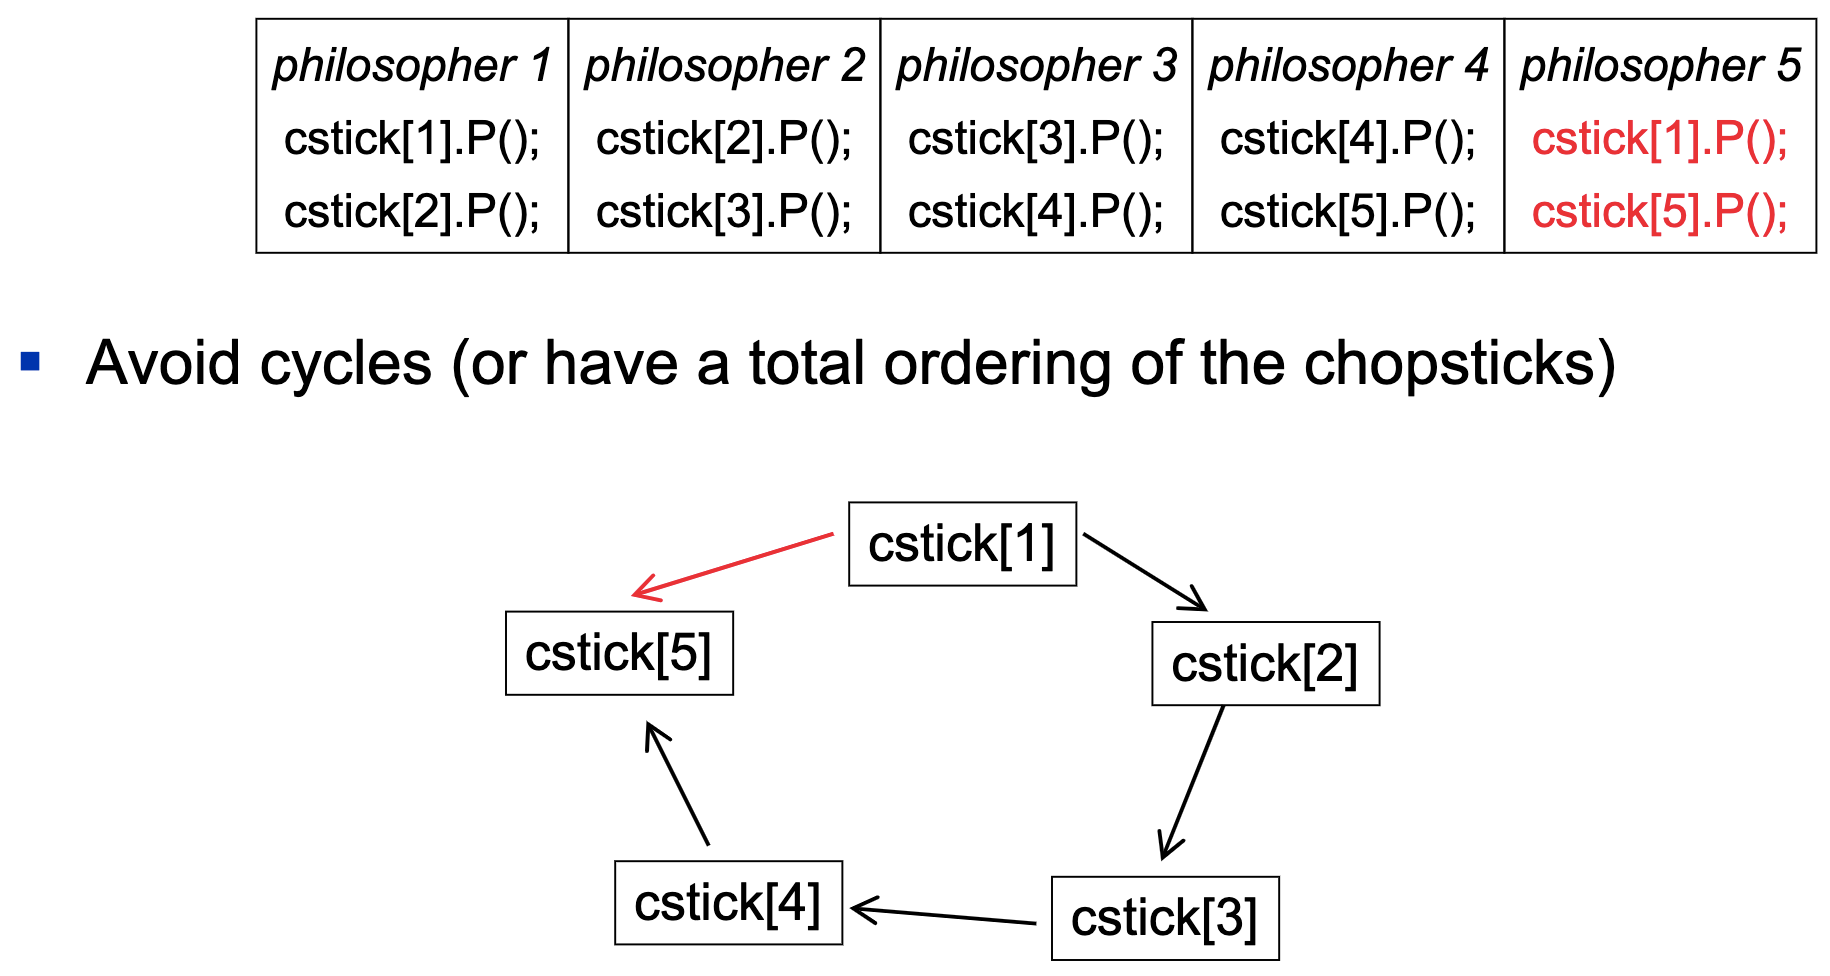
\includegraphics[width=0.49\linewidth]{cs4231-dining-philosophers-1.png} 
  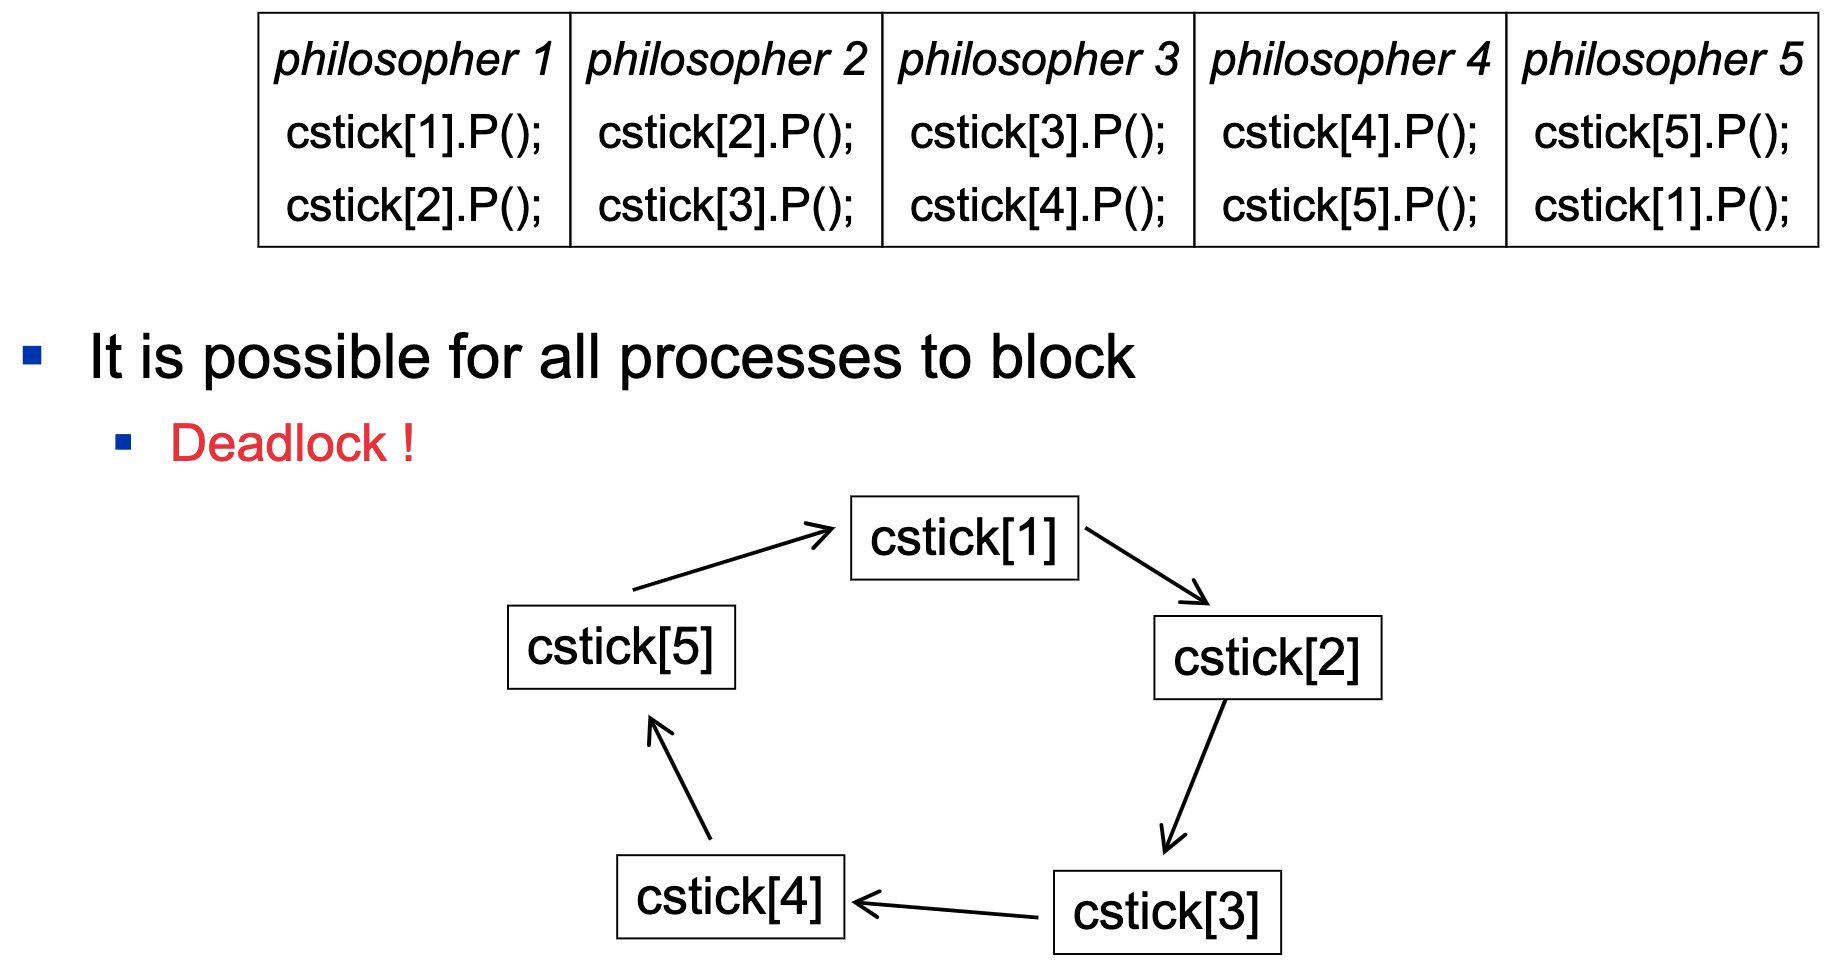
\includegraphics[width=0.49\linewidth]{cs4231-dining-philosophers-2.png} 

  \subsection{Monitor}

  \begin{itemize}
    \item $\checkmark$ higher-level/easier to use than semaphore
    \item every object in Java is a monitor
  \end{itemize}

  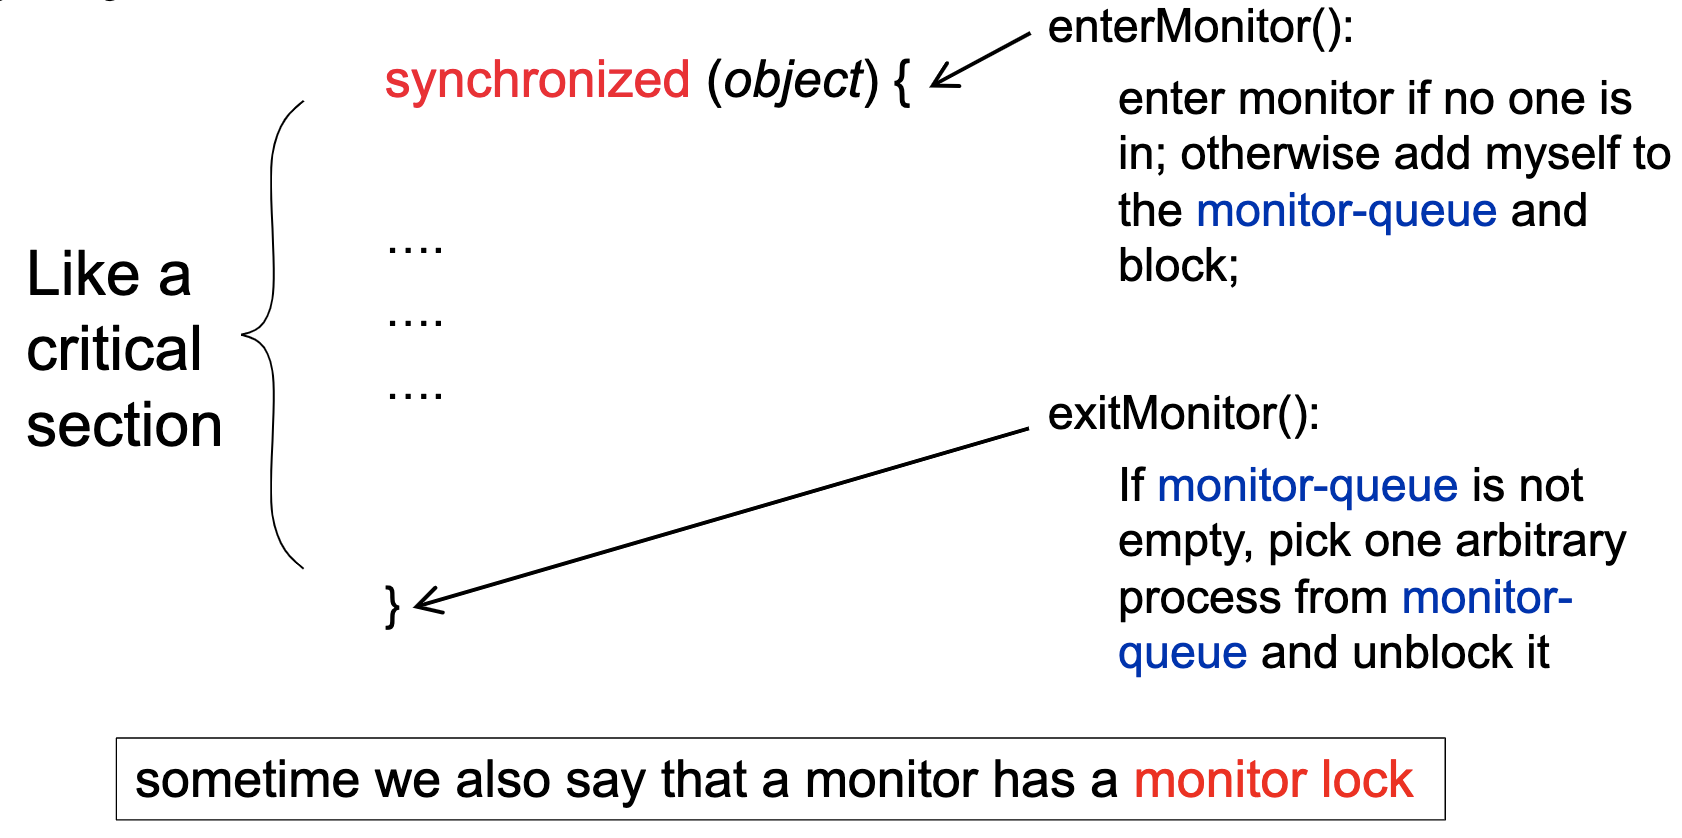
\includegraphics[width=0.49\linewidth]{cs4231-monitor-1.png} 
  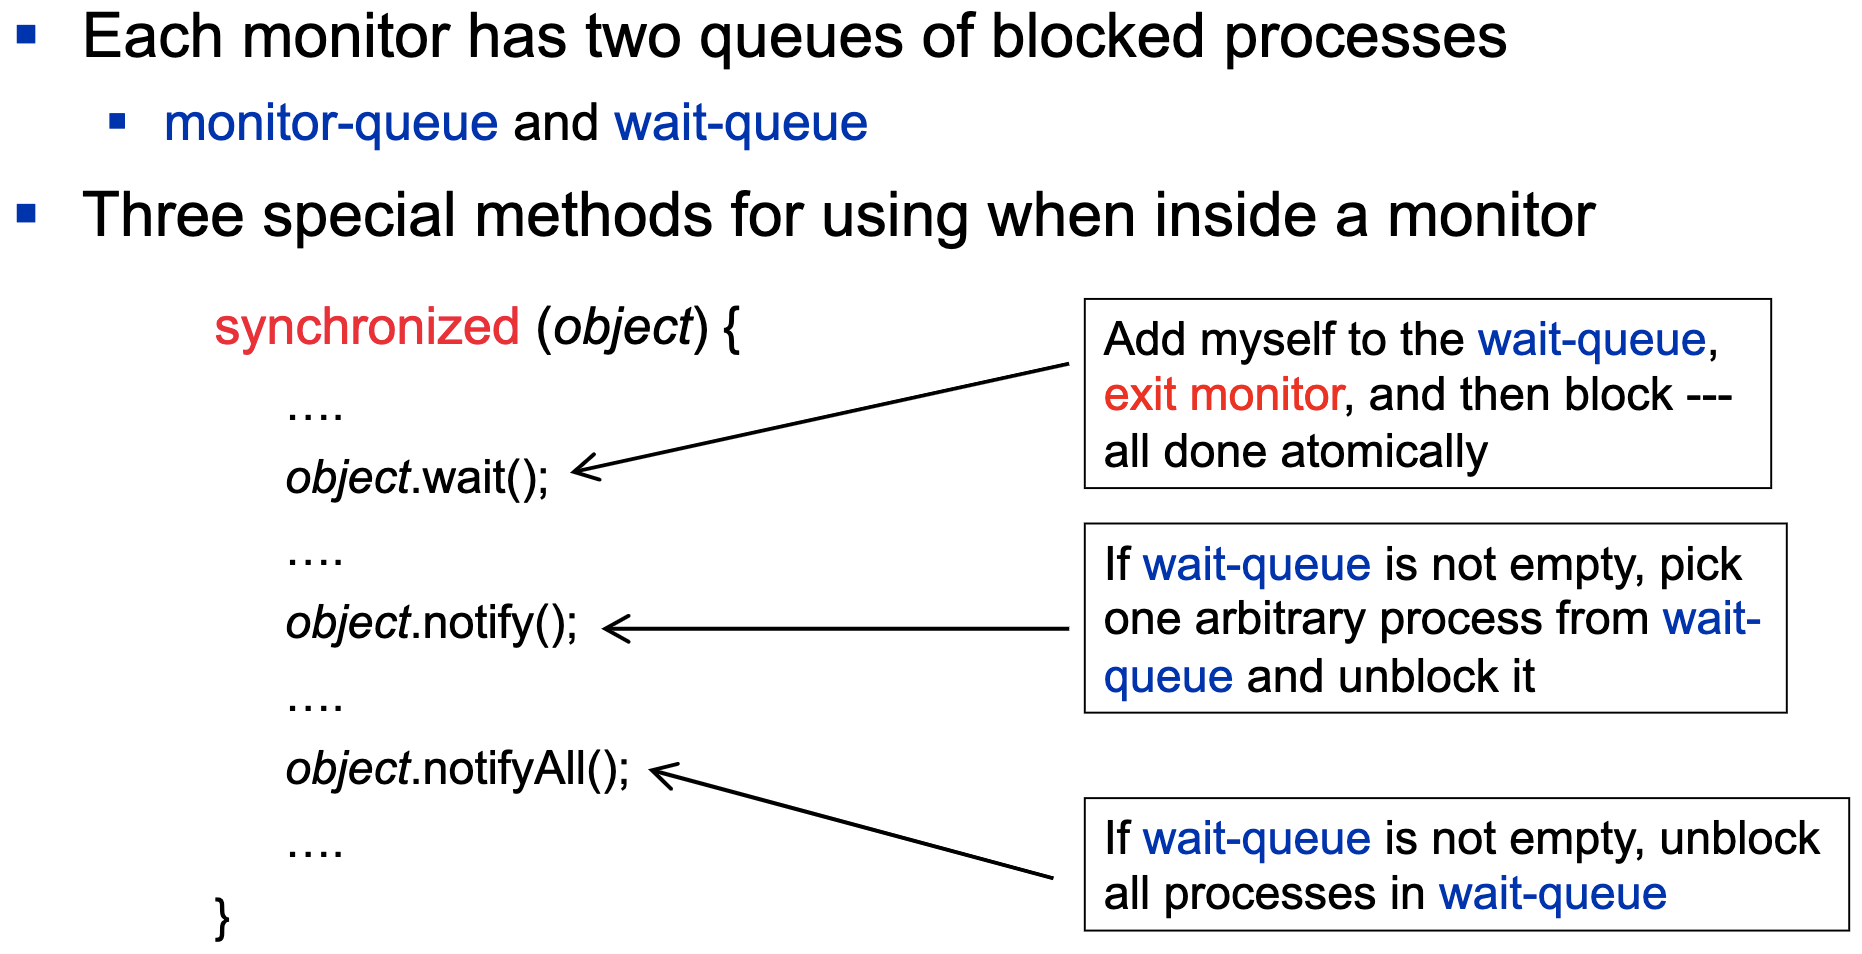
\includegraphics[width=0.49\linewidth]{cs4231-monitor-2.png} 

  \begin{multicols*}{2}

    \subsubsection{Hoare-style}

    \begin{itemize}
      \item \texttt{notify()} immediately switches from caller to a waiting thread
      \item doesn't use \texttt{notifyAll()}
    \end{itemize}

    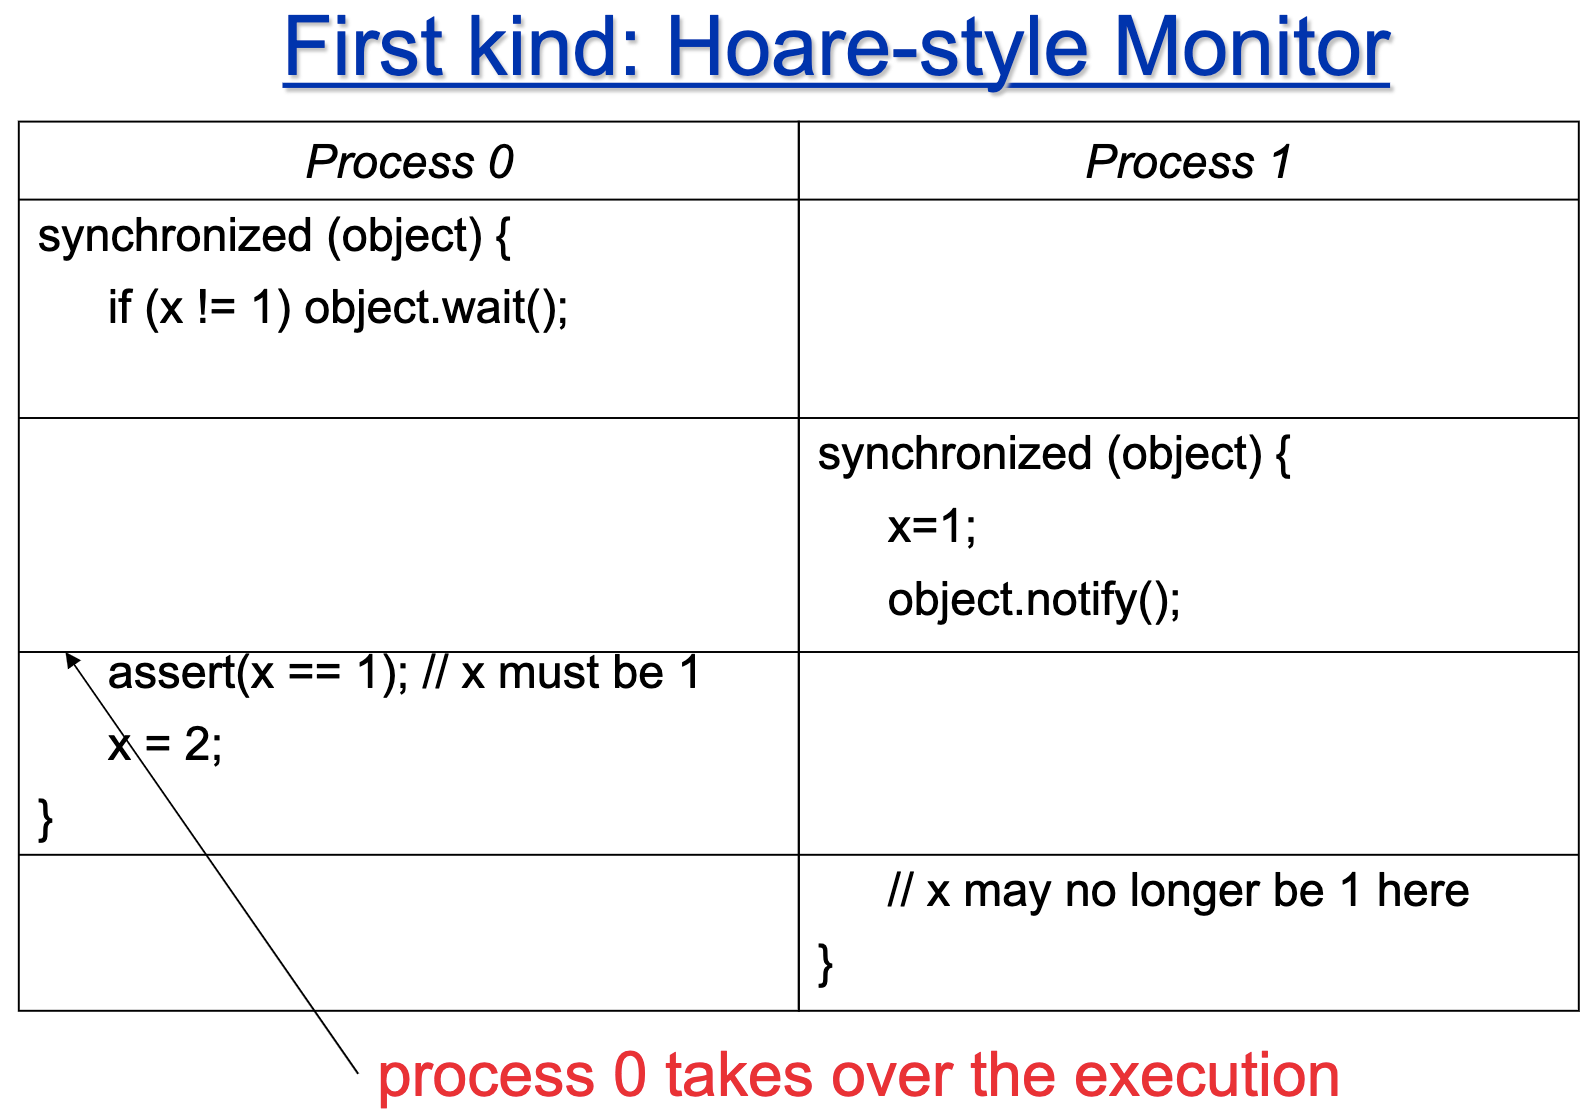
\includegraphics[width=\linewidth]{cs4231-monitor-hoare.png} 

    \ \\ \ 

    \subsubsection{Java-style}

    \begin{itemize}
      \item \texttt{notify()} places a waiter on the ready thread but signaller continues inside the monitor
    \end{itemize}

    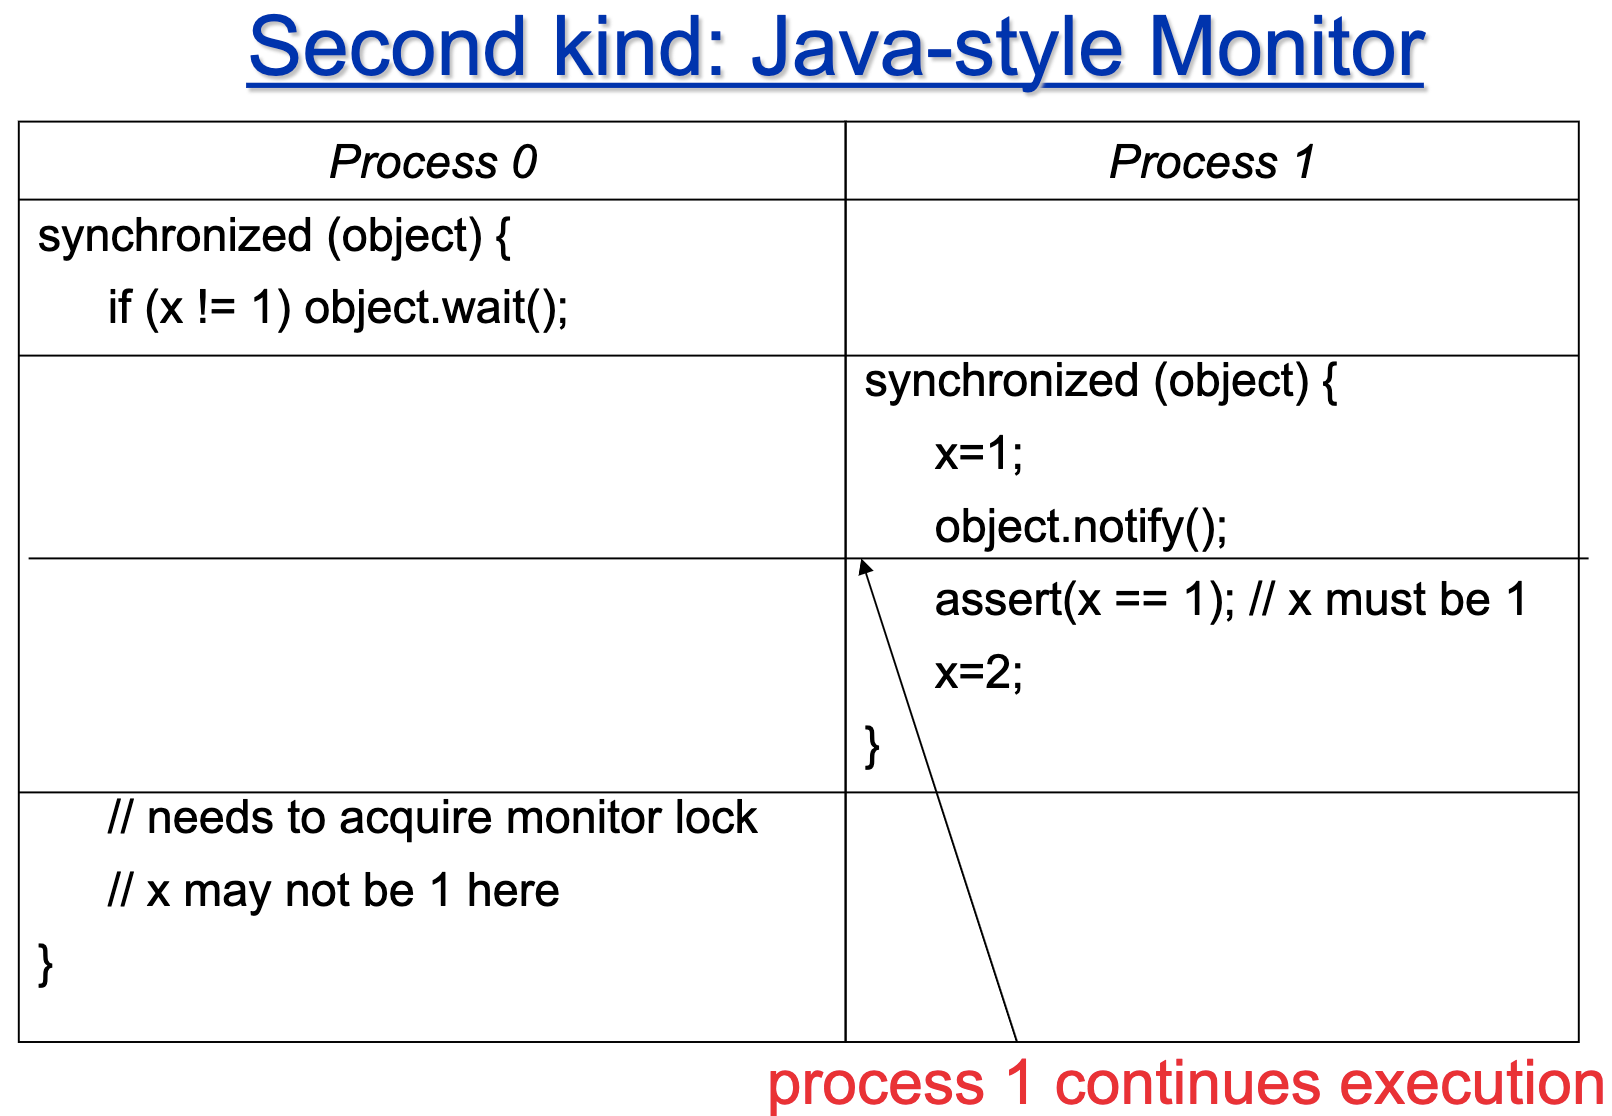
\includegraphics[width=\linewidth]{cs4231-monitor-java.png} 

    \begin{itemize}
      \item P0 must acquire monitor lock
        \begin{itemize}
          \item use \texttt{(while x!=1)} to ensure \texttt{x==1}
        \end{itemize}
    \end{itemize}

  \end{multicols*}

  \subsubsection{nested monitor}

  \begin{itemize}
    \item \texttt{wait()} only releases the \textit{immediate} monitor lock
  \end{itemize}
  \begin{tightcenter}
    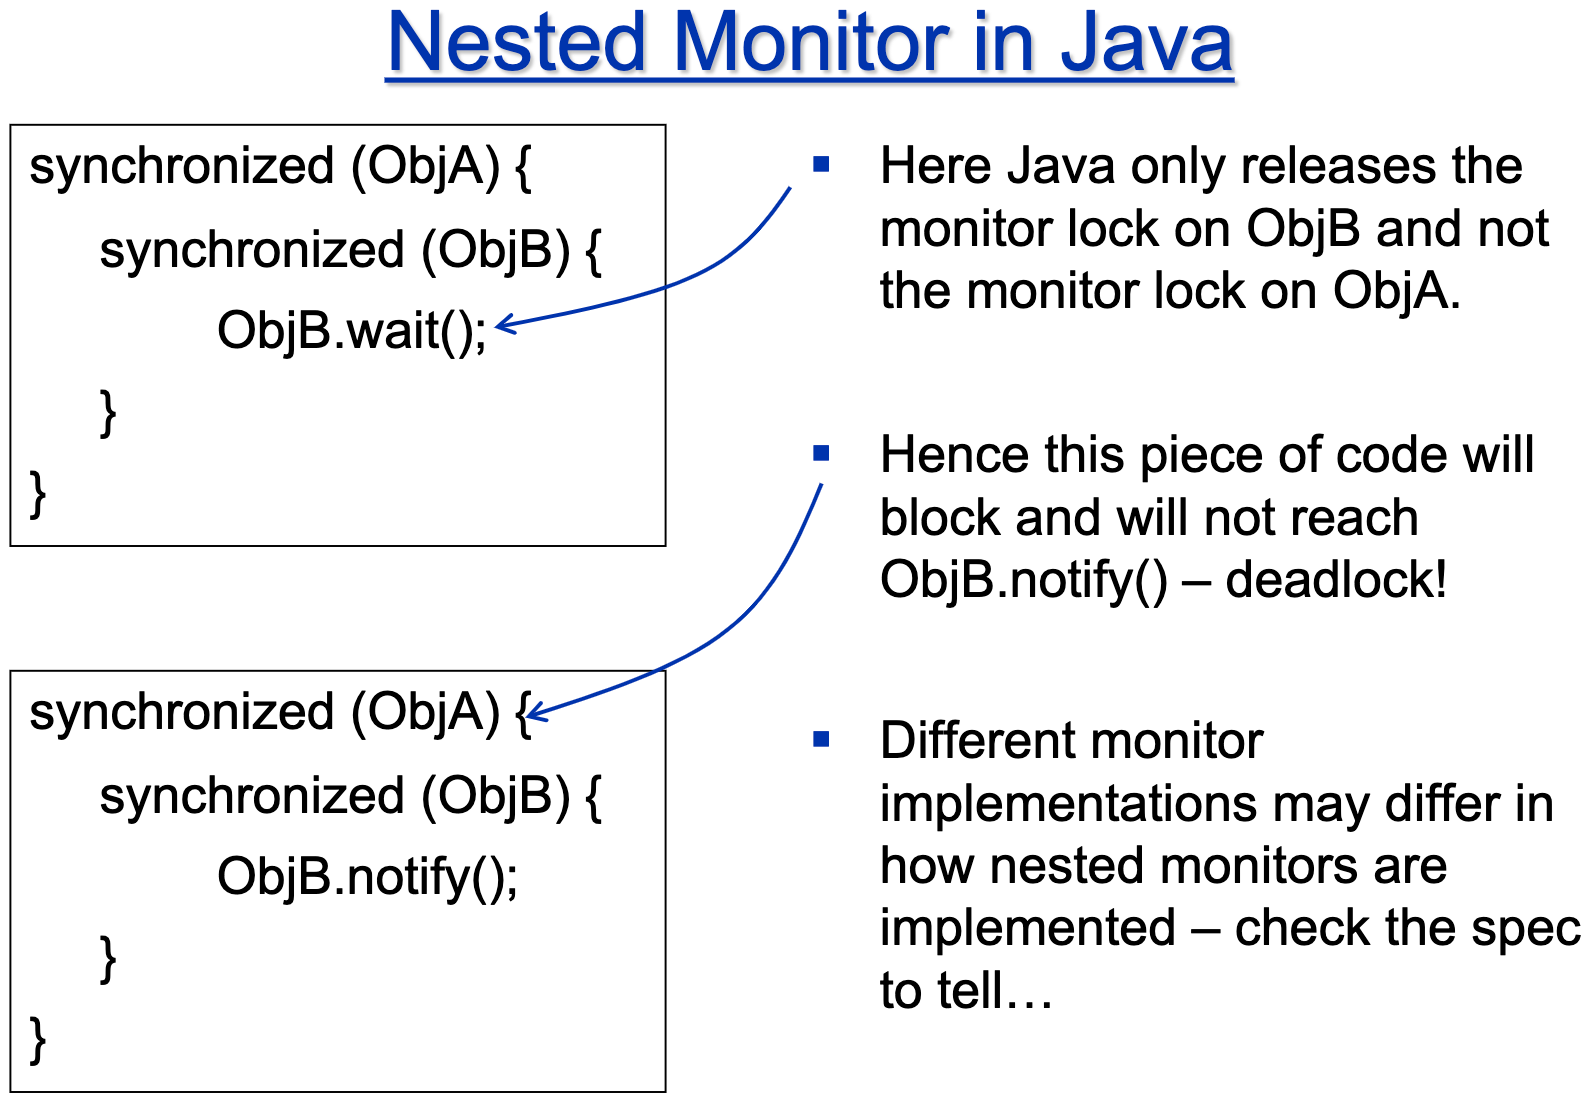
\includegraphics[width=0.7\linewidth]{cs4231-nested-monitor.png} 
  \end{tightcenter}

  \subsubsection{producer-consumer problem}

  \begin{itemize}
    \item circular buffer of size $n$
    \item single producer, single consumer
      \begin{itemize}
        \item producer places item to the end of the buffer if buffer is not full
        \item consumer removes item from the head of the buffer if not empty
      \end{itemize}
  \end{itemize}

  \begin{tightcenter}
    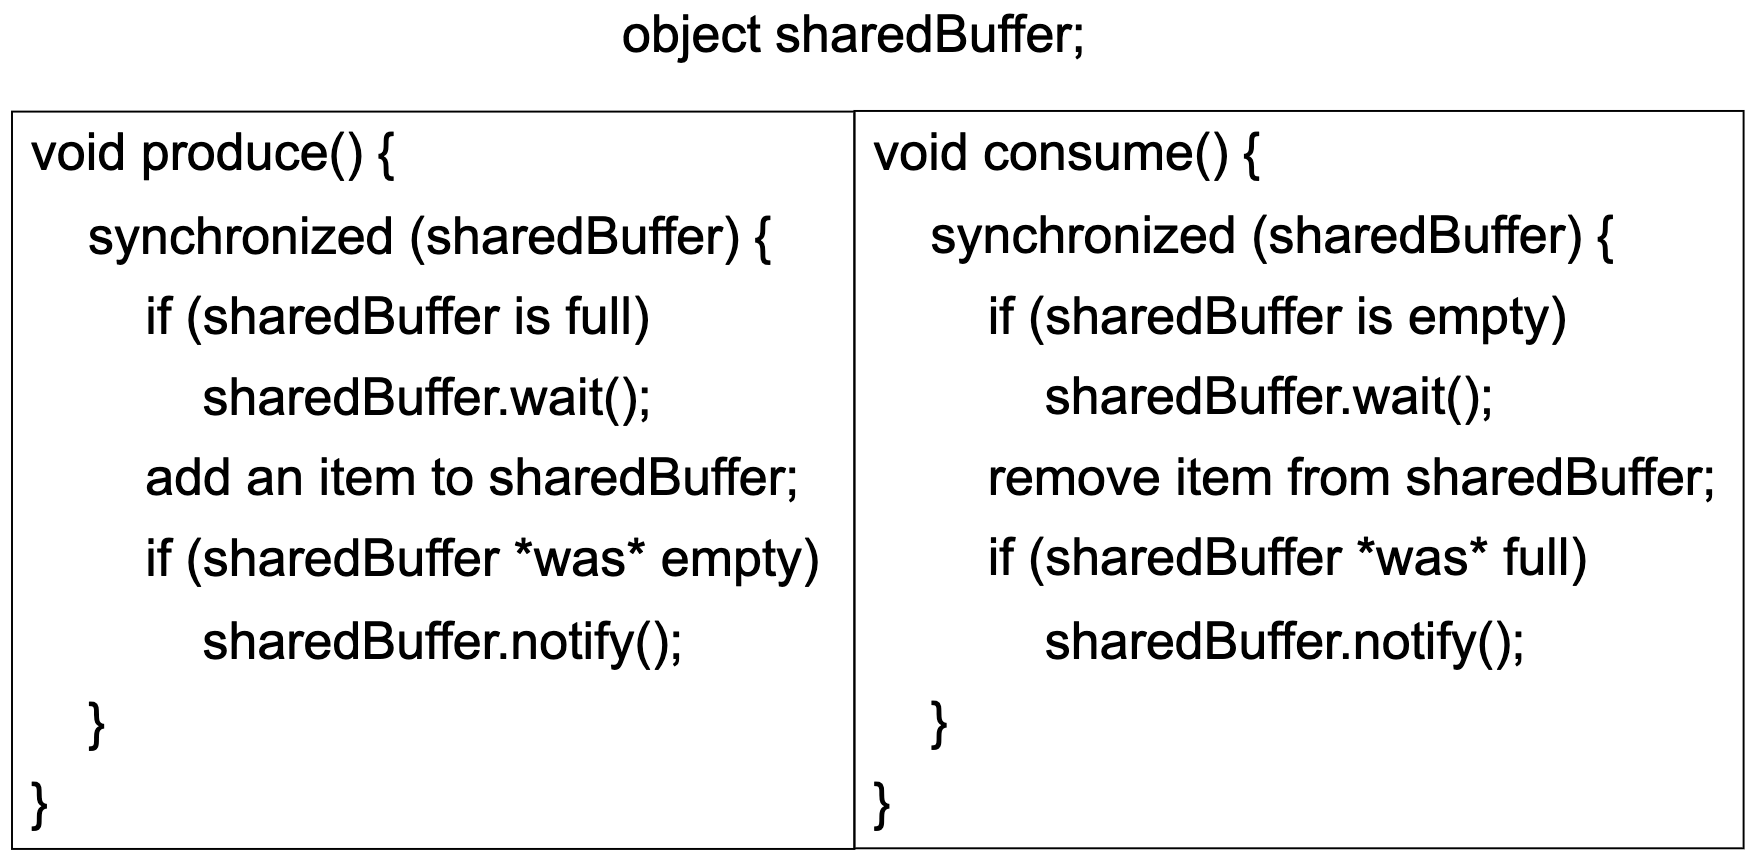
\includegraphics[width=0.8\linewidth]{cs4231-producer-consumer-monitor.png} 
  \end{tightcenter}

  \subsubsection{reader-writer problem}

  \begin{itemize}
    \item multiple readers and writers accessing a file
      \begin{itemize}
        \item writer must have exclusive access
        \item readers may simultaneously access the file
      \end{itemize}
  \end{itemize}

  \begin{tightcenter}
    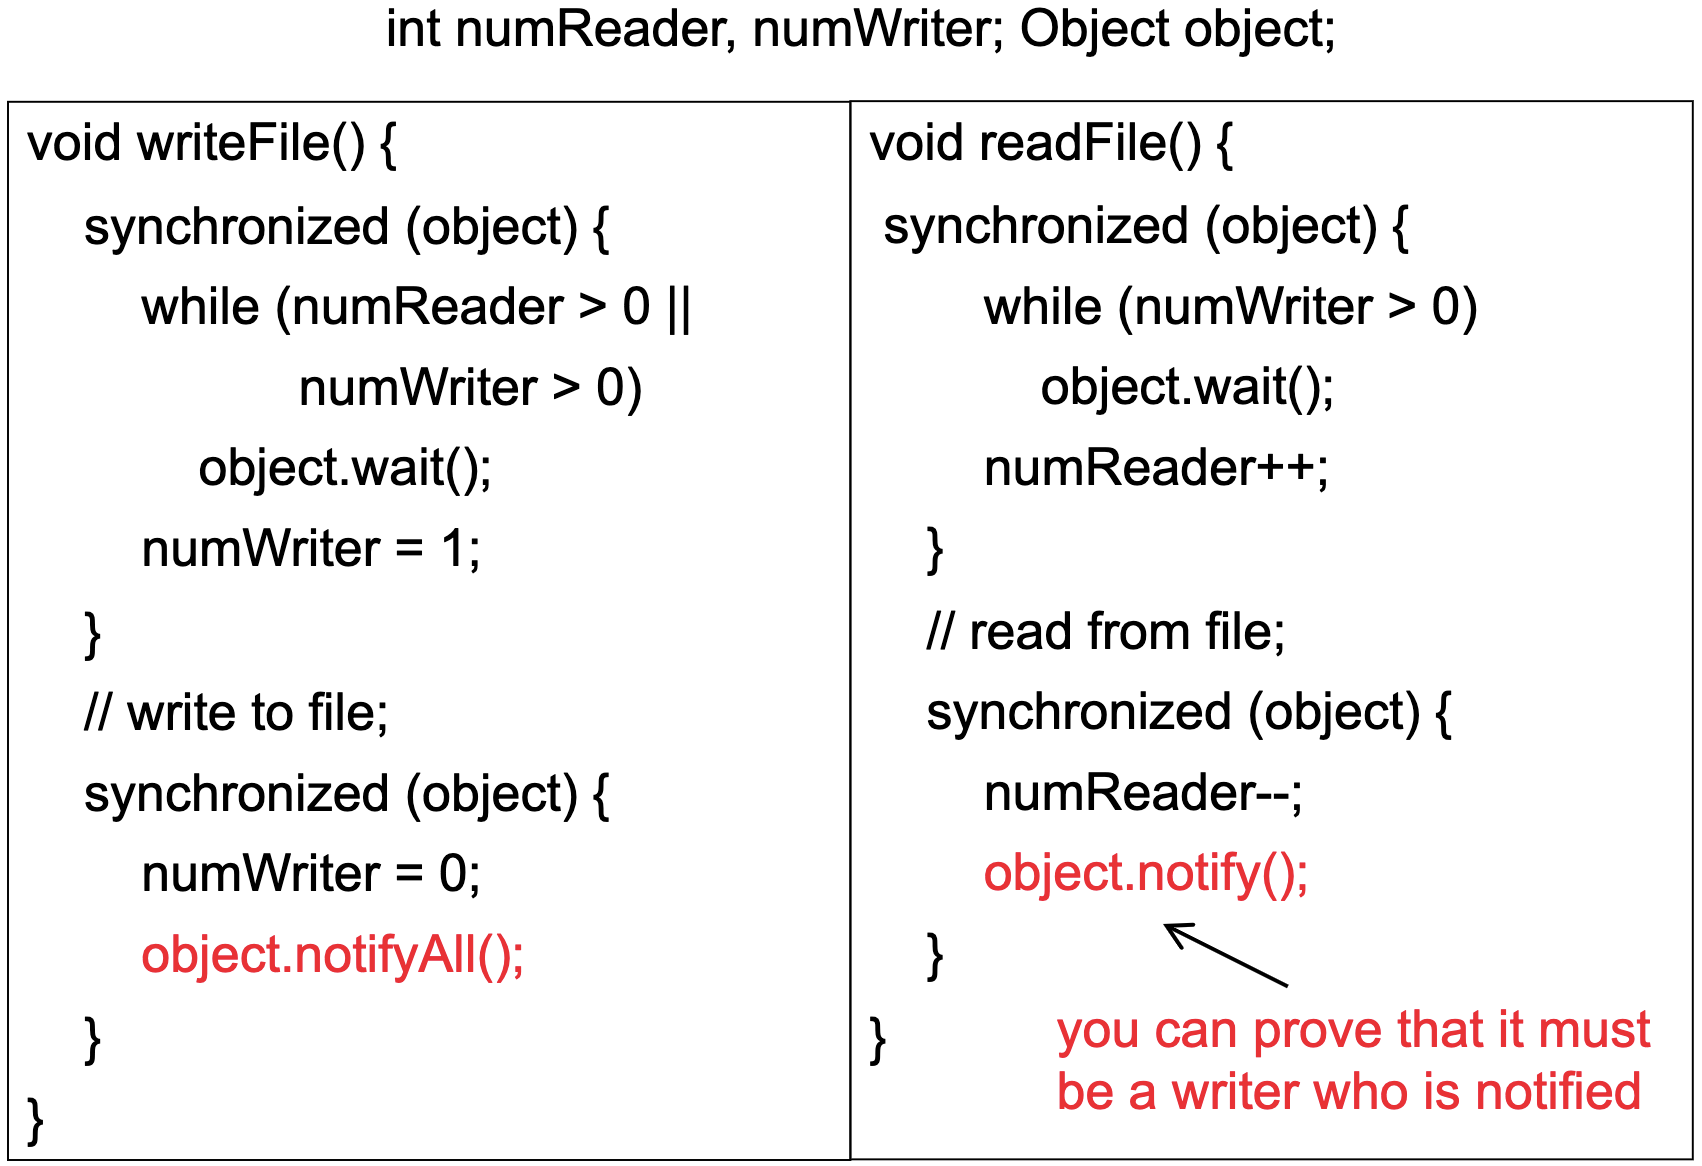
\includegraphics[width=0.7\linewidth]{cs4231-reader-writer-monitor.png} 
  \end{tightcenter}

  \vfill\null
  \columnbreak

  \subsubsection{reader-writer (without starvation)}

  maintain an explicit queue

  \begin{tightcenter}
    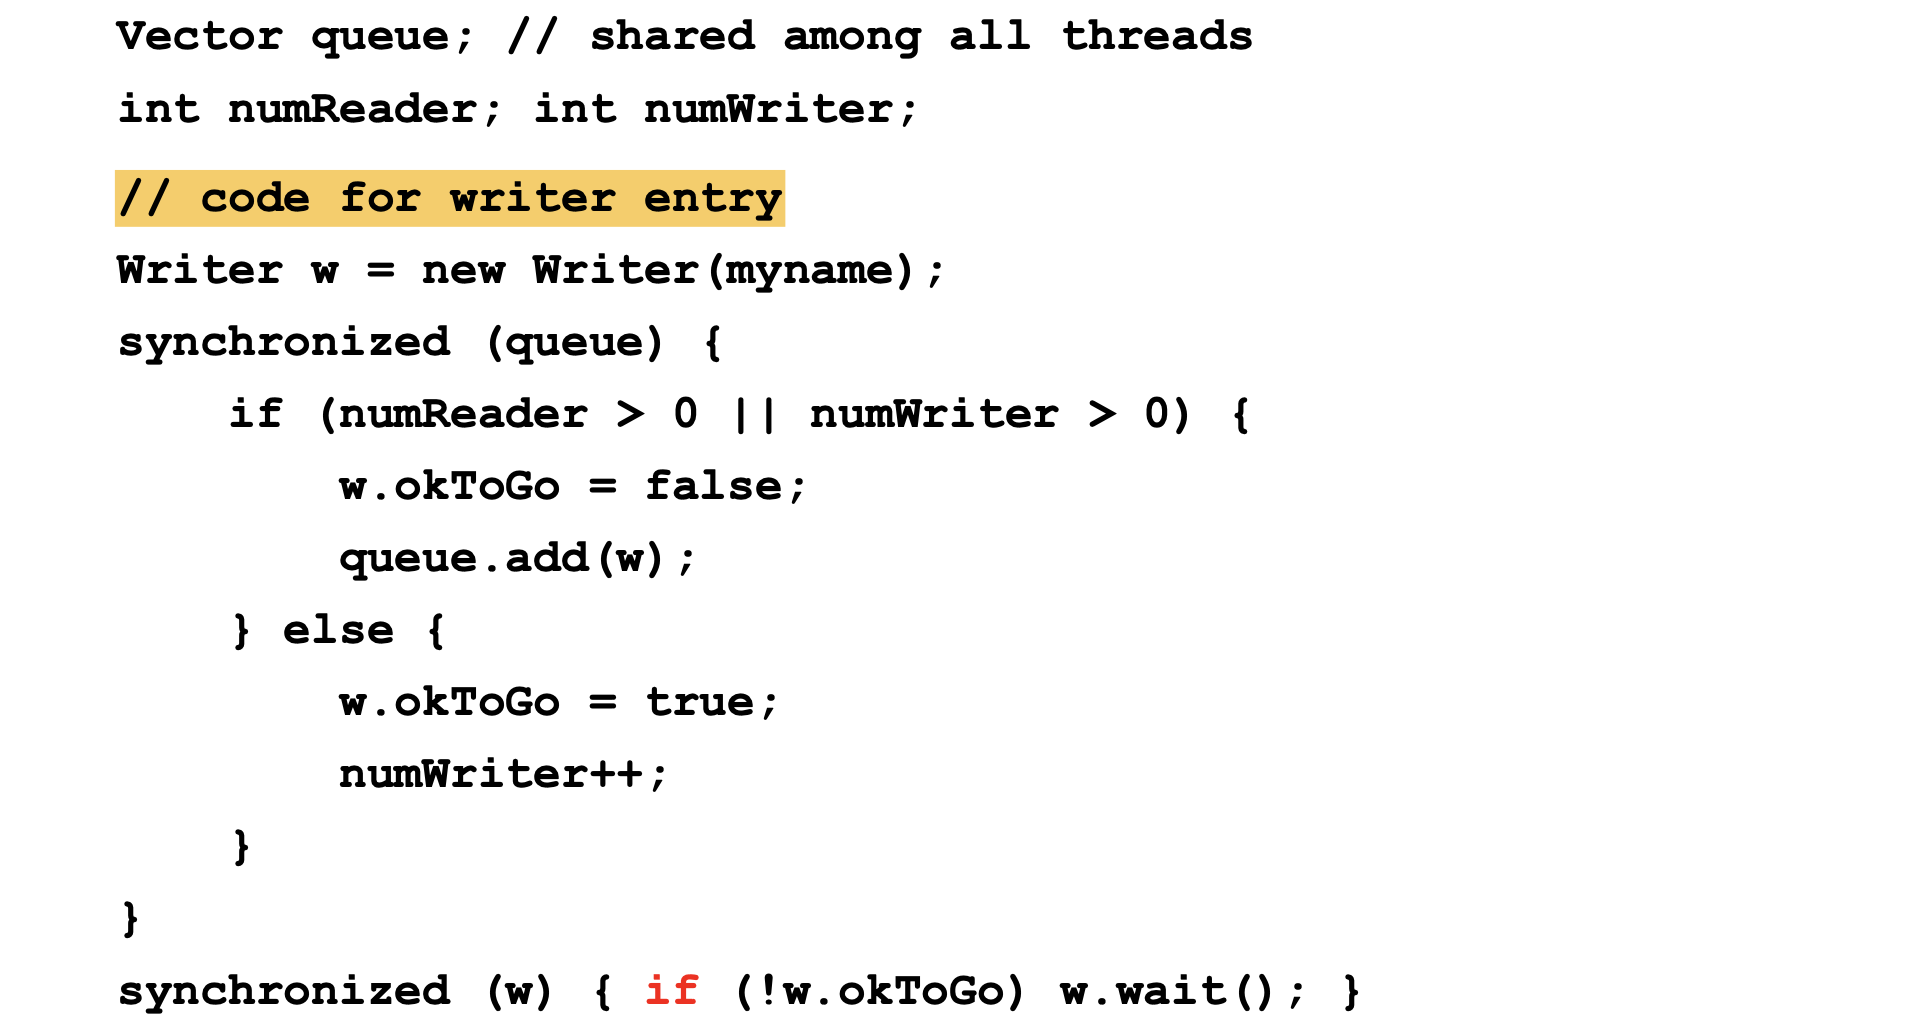
\includegraphics[width=0.9\linewidth]{cs4231-reader-writer-no-starvation-1.png} 
    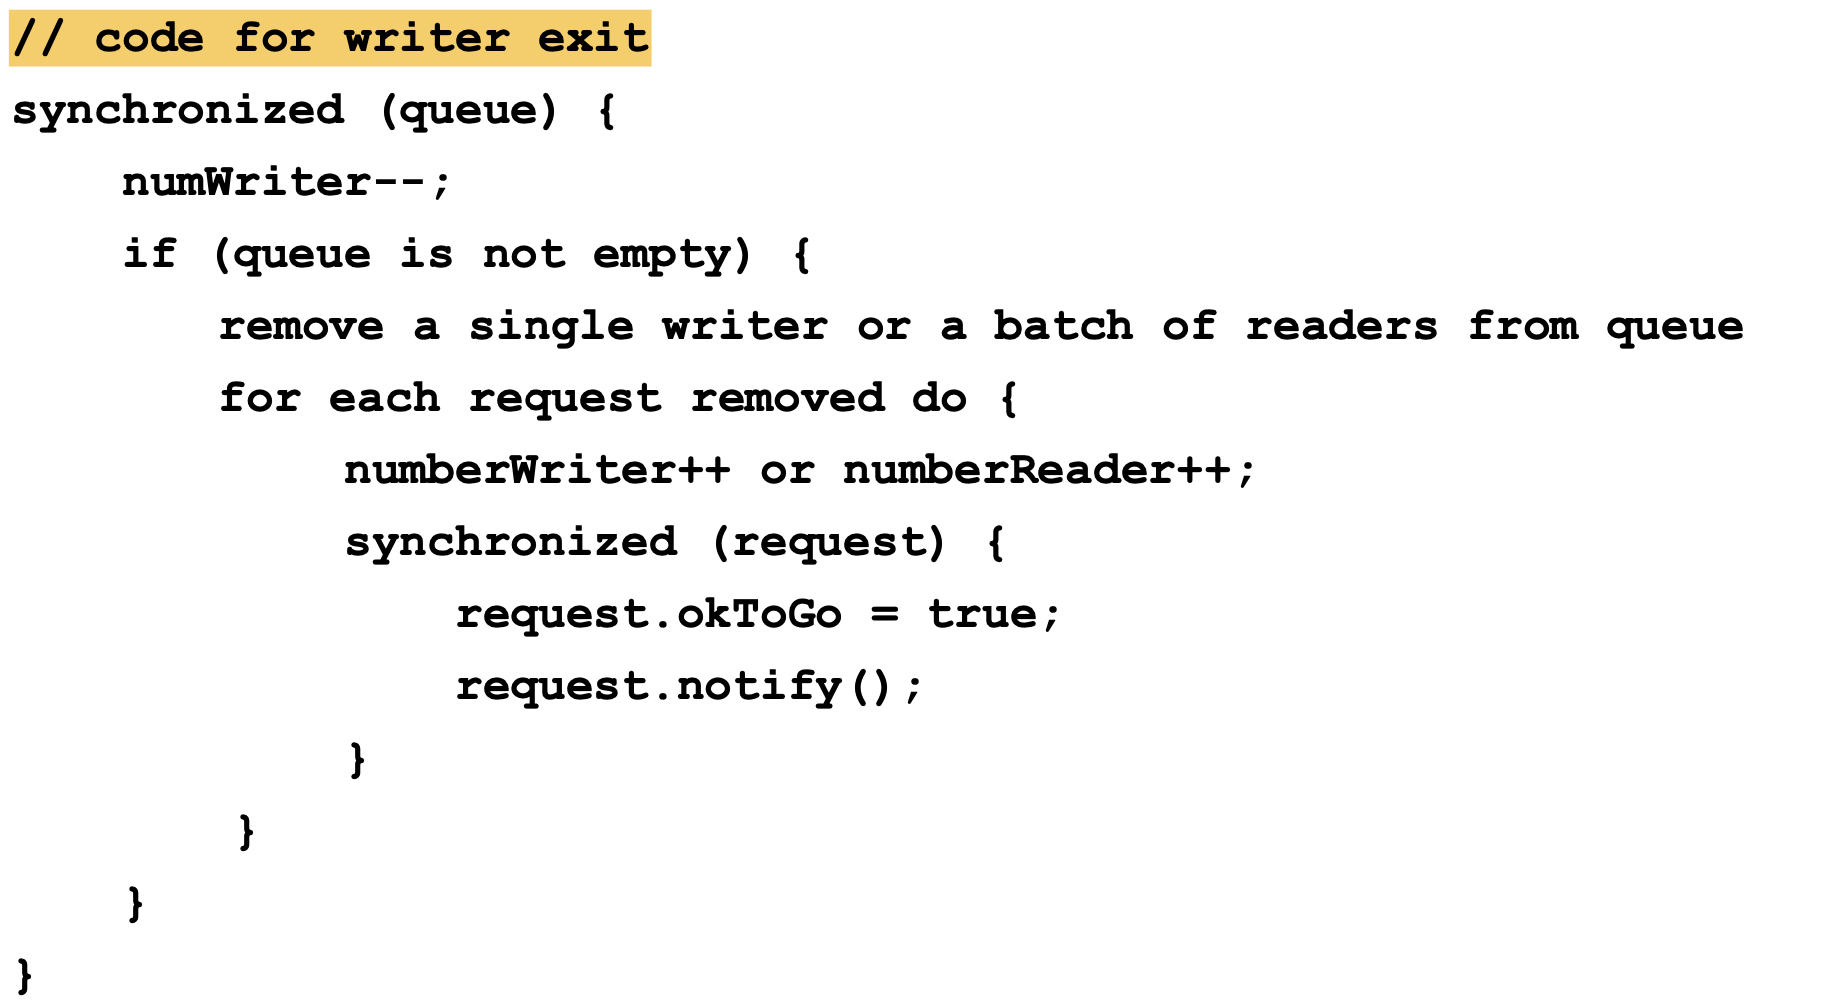
\includegraphics[width=0.9\linewidth]{cs4231-reader-writer-no-starvation-2.png} 
    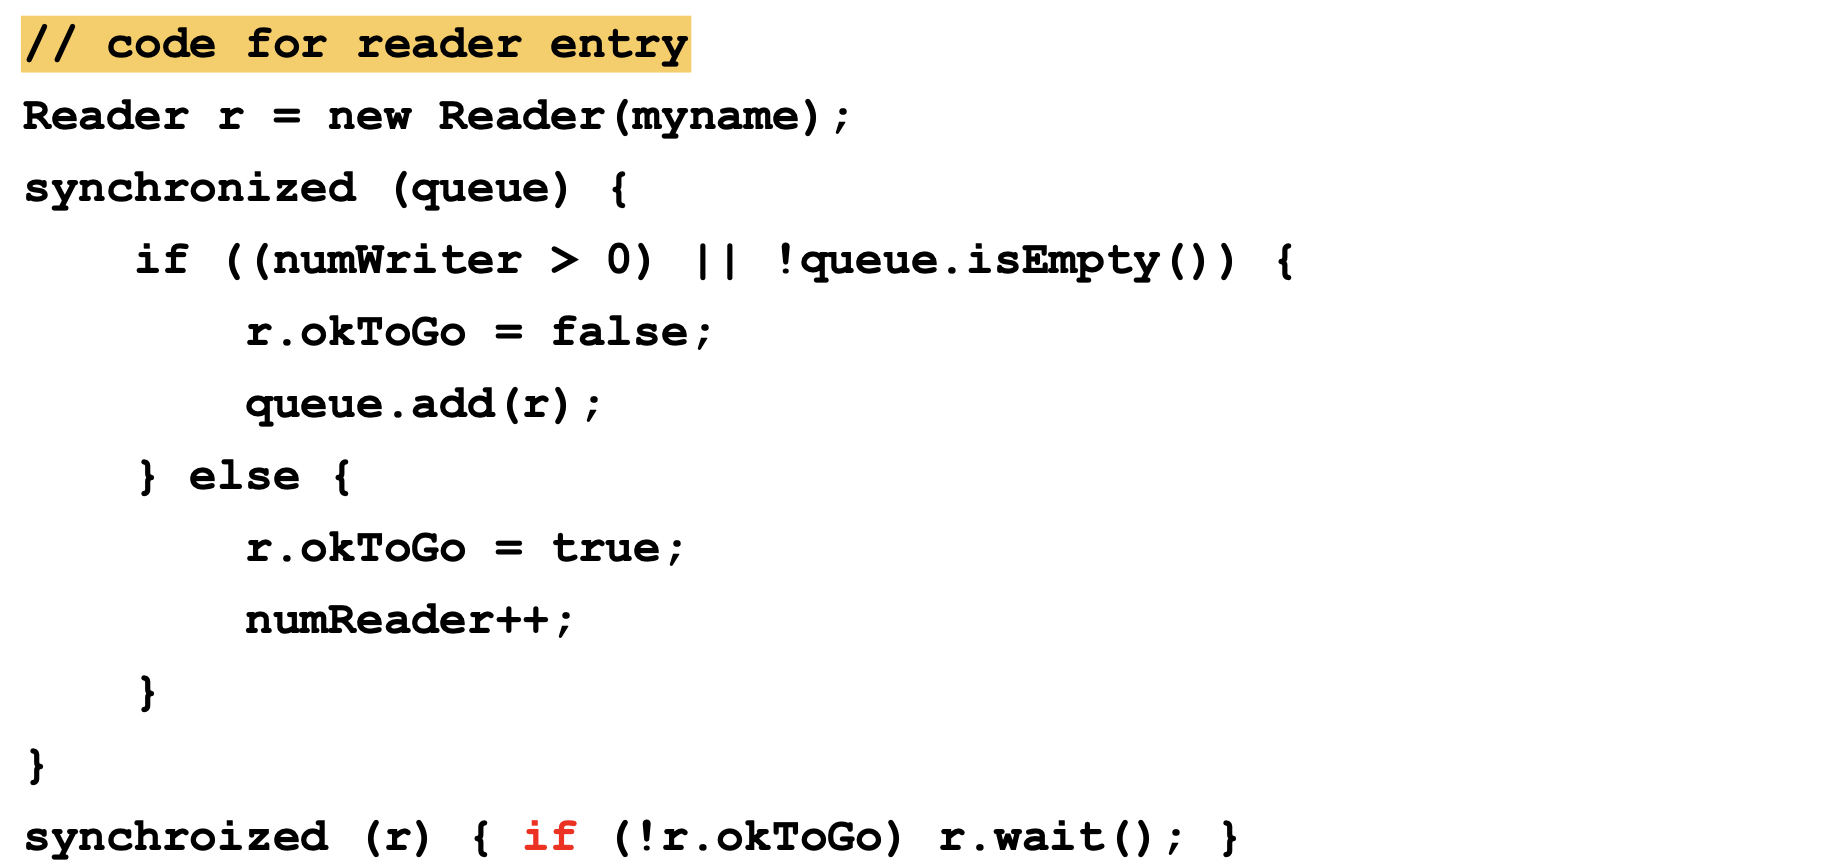
\includegraphics[width=0.9\linewidth]{cs4231-reader-writer-no-starvation-3.png} 
    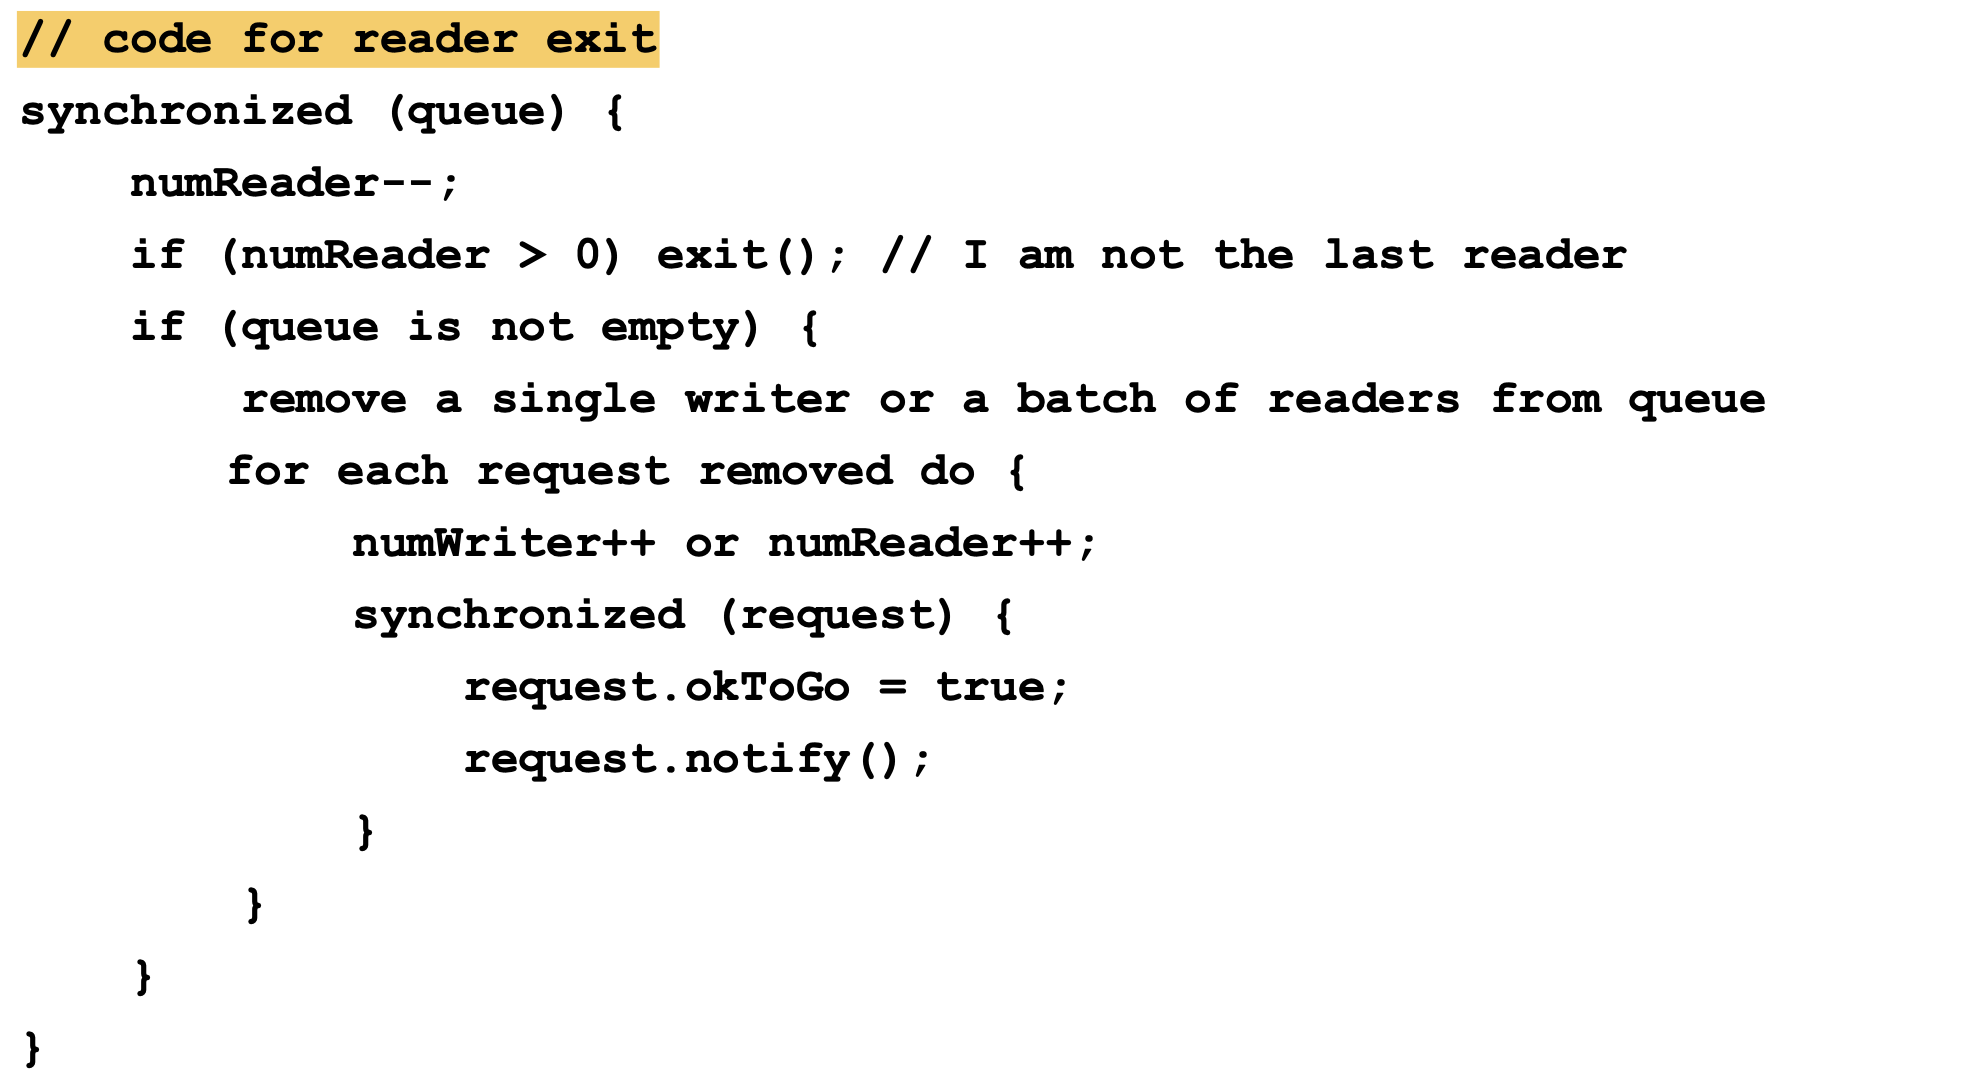
\includegraphics[width=0.9\linewidth]{cs4231-reader-writer-no-starvation-4.png} 
  \end{tightcenter}

  \vfill\null
  \columnbreak

  \subsubsection{barber-shop problem}

  \begin{tightcenter}
    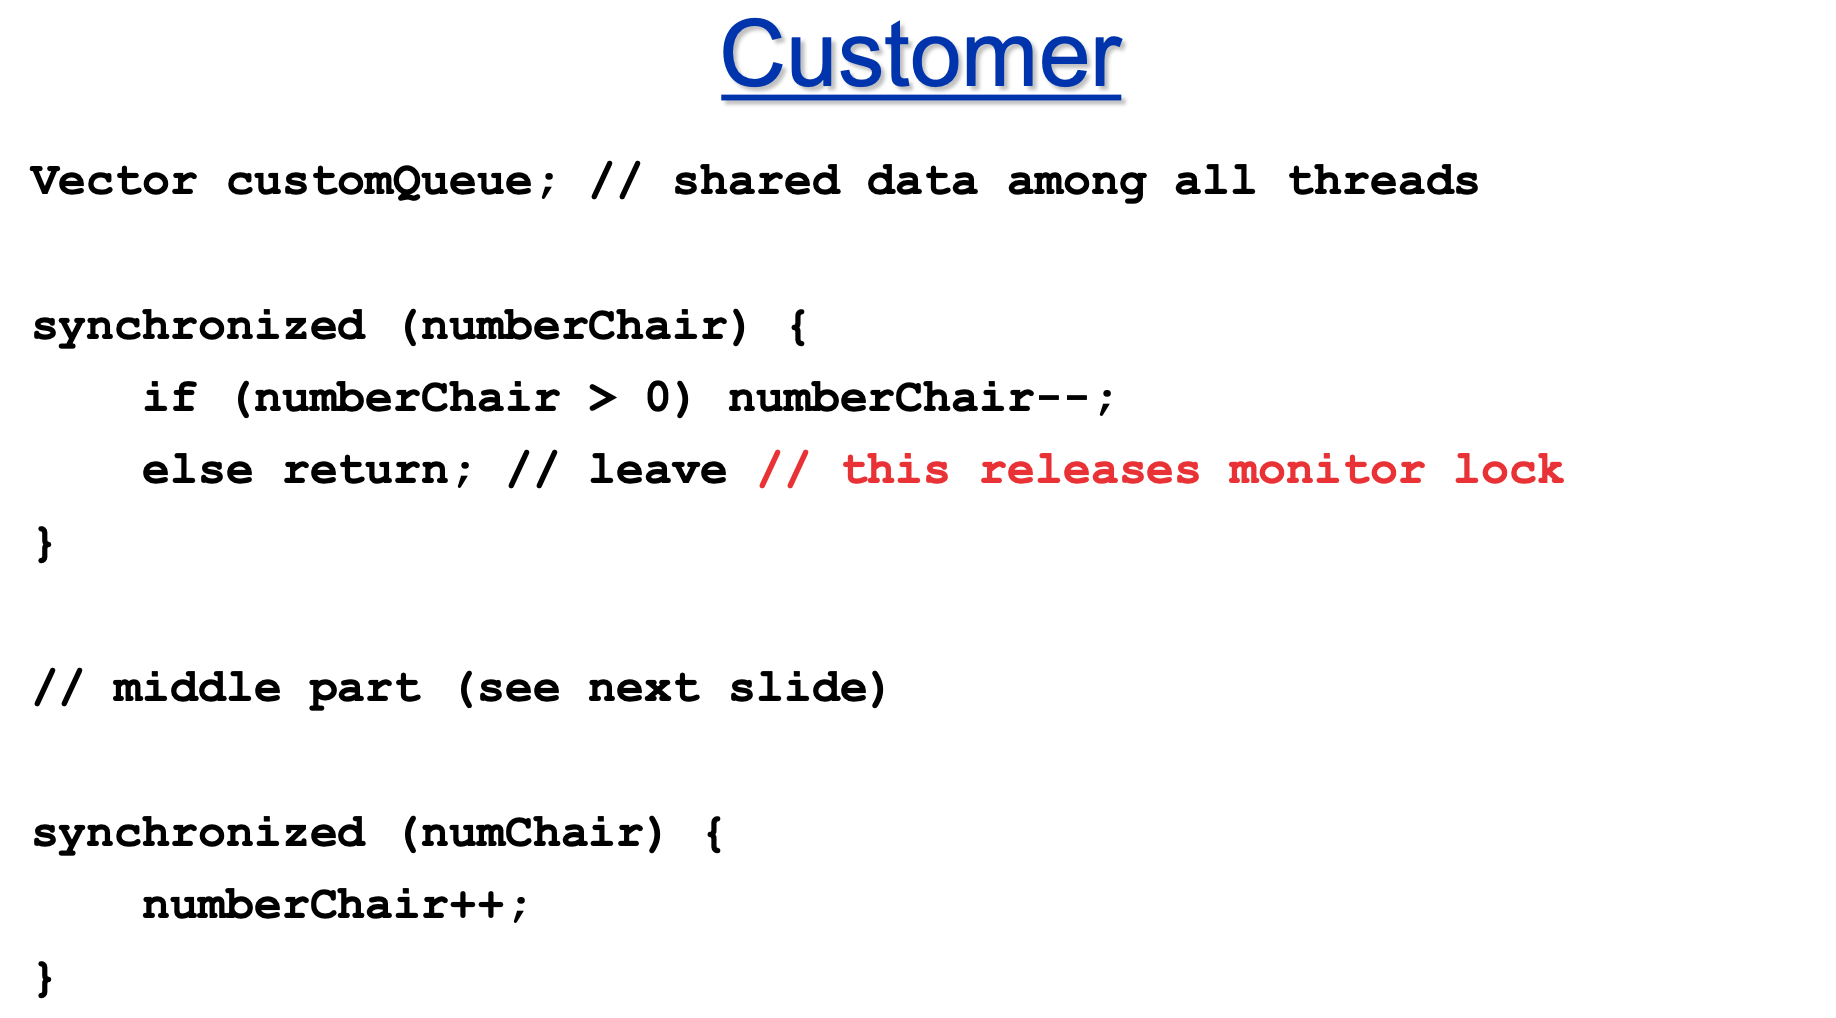
\includegraphics[width=0.9\linewidth]{cs4231-barbershop-1.png} 
    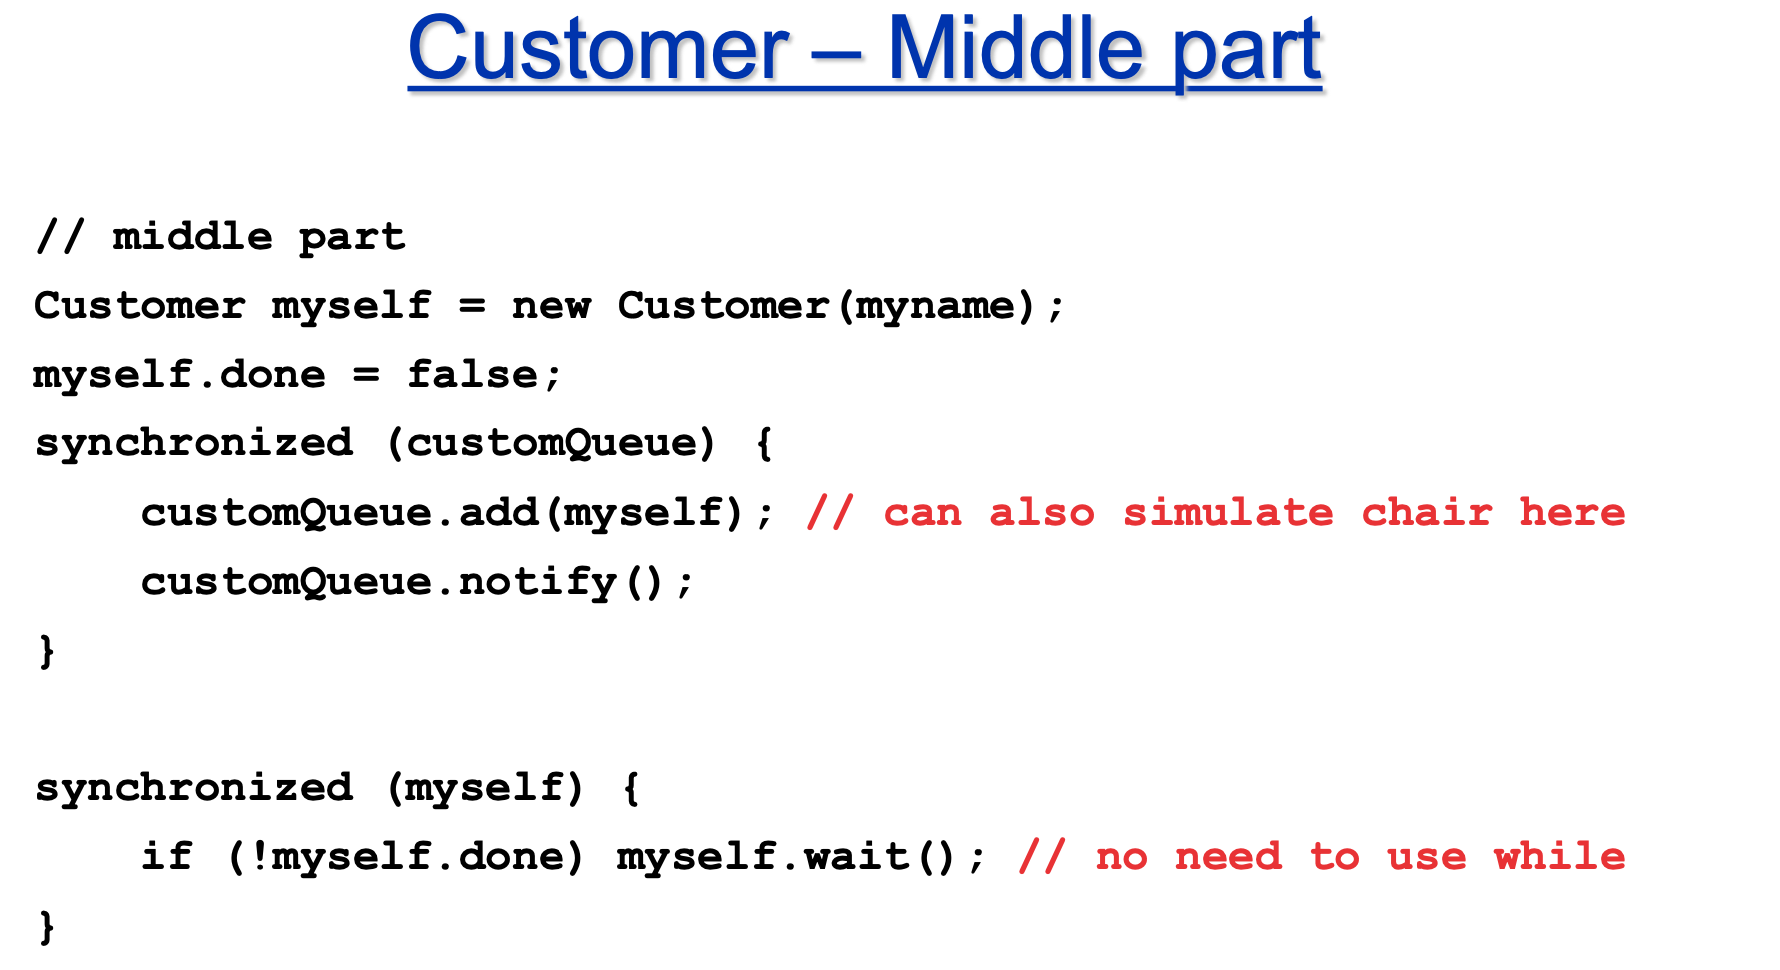
\includegraphics[width=0.9\linewidth]{cs4231-barbershop-2.png} 
    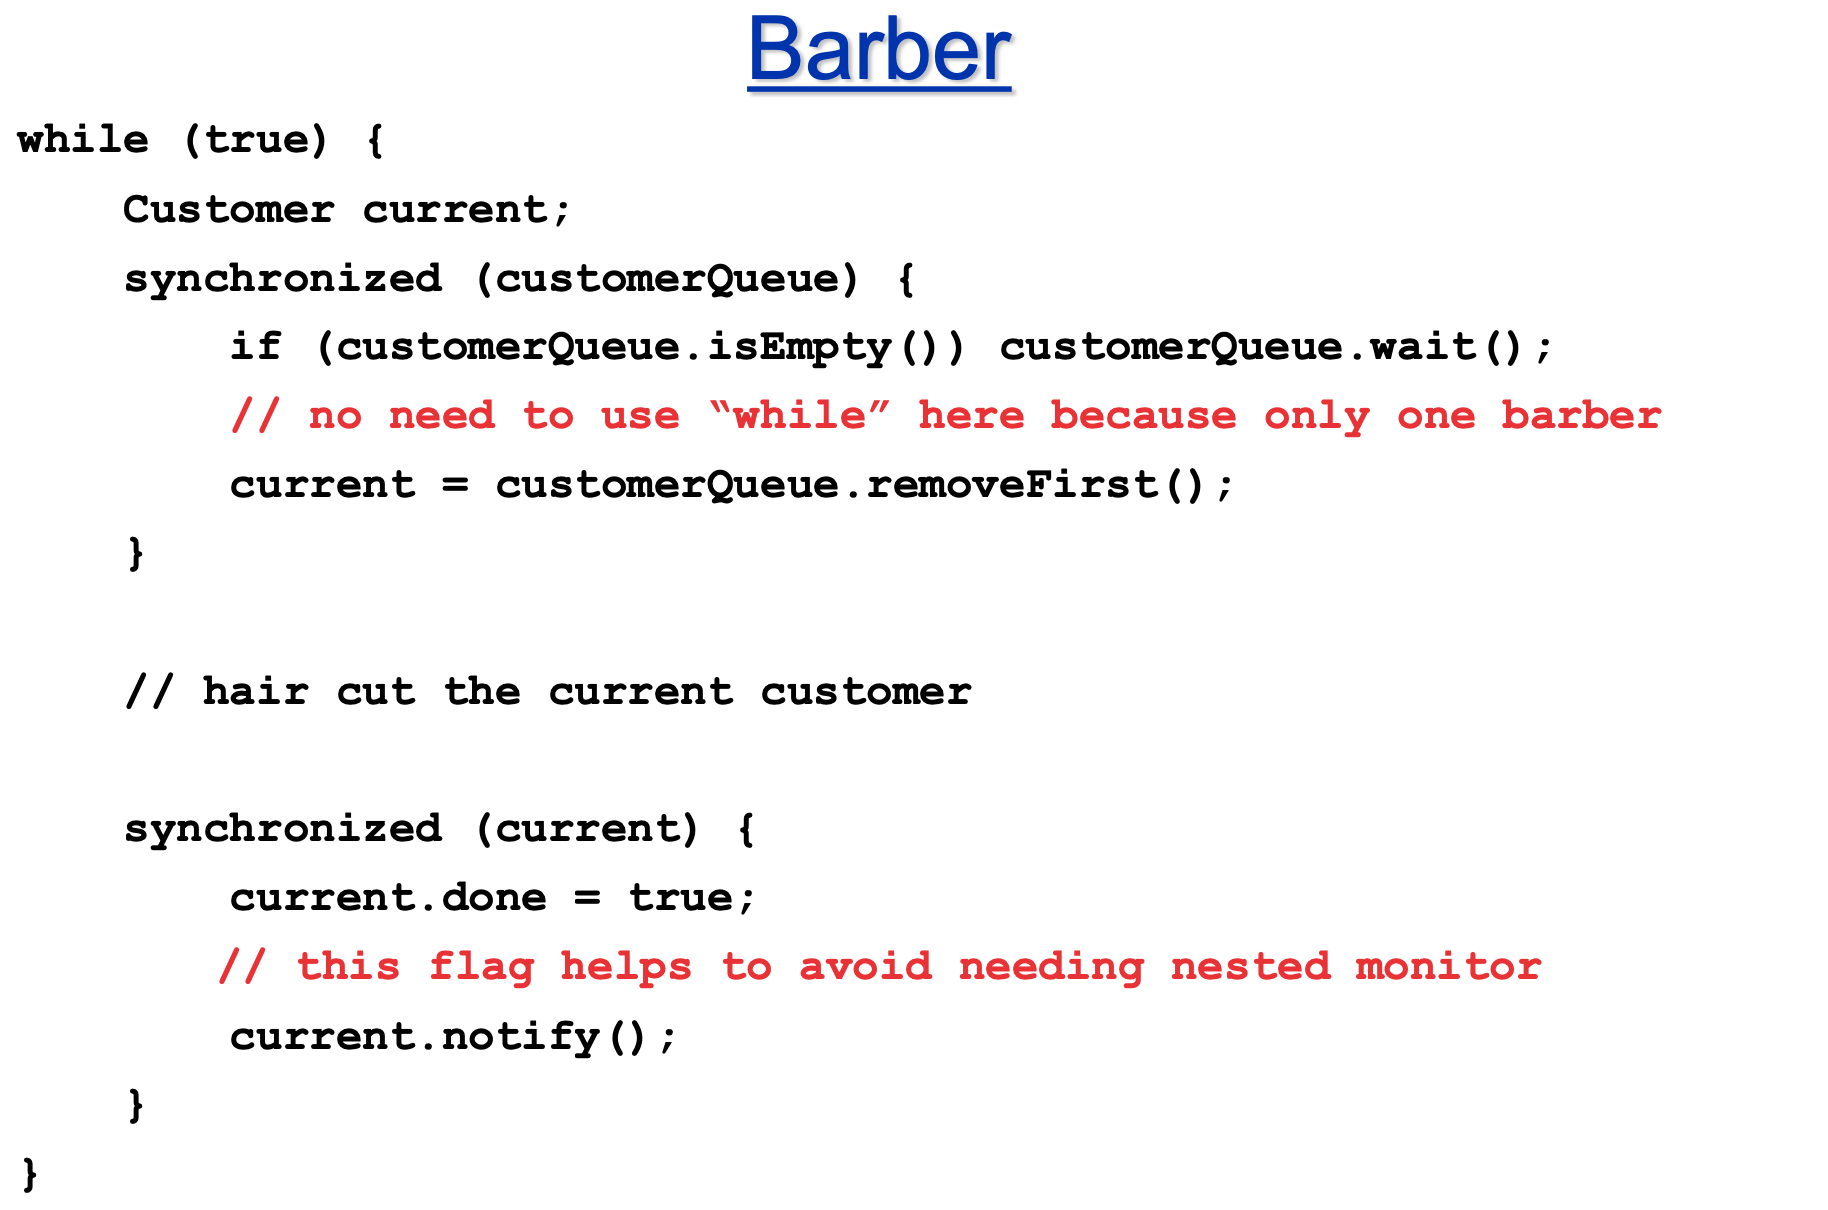
\includegraphics[width=0.9\linewidth]{cs4231-barbershop-3.png} 
  \end{tightcenter}

  \vfill\null
  \columnbreak

  \section{03. CONSISTENCY CONDITIONS}

  \begin{tightcenter}
    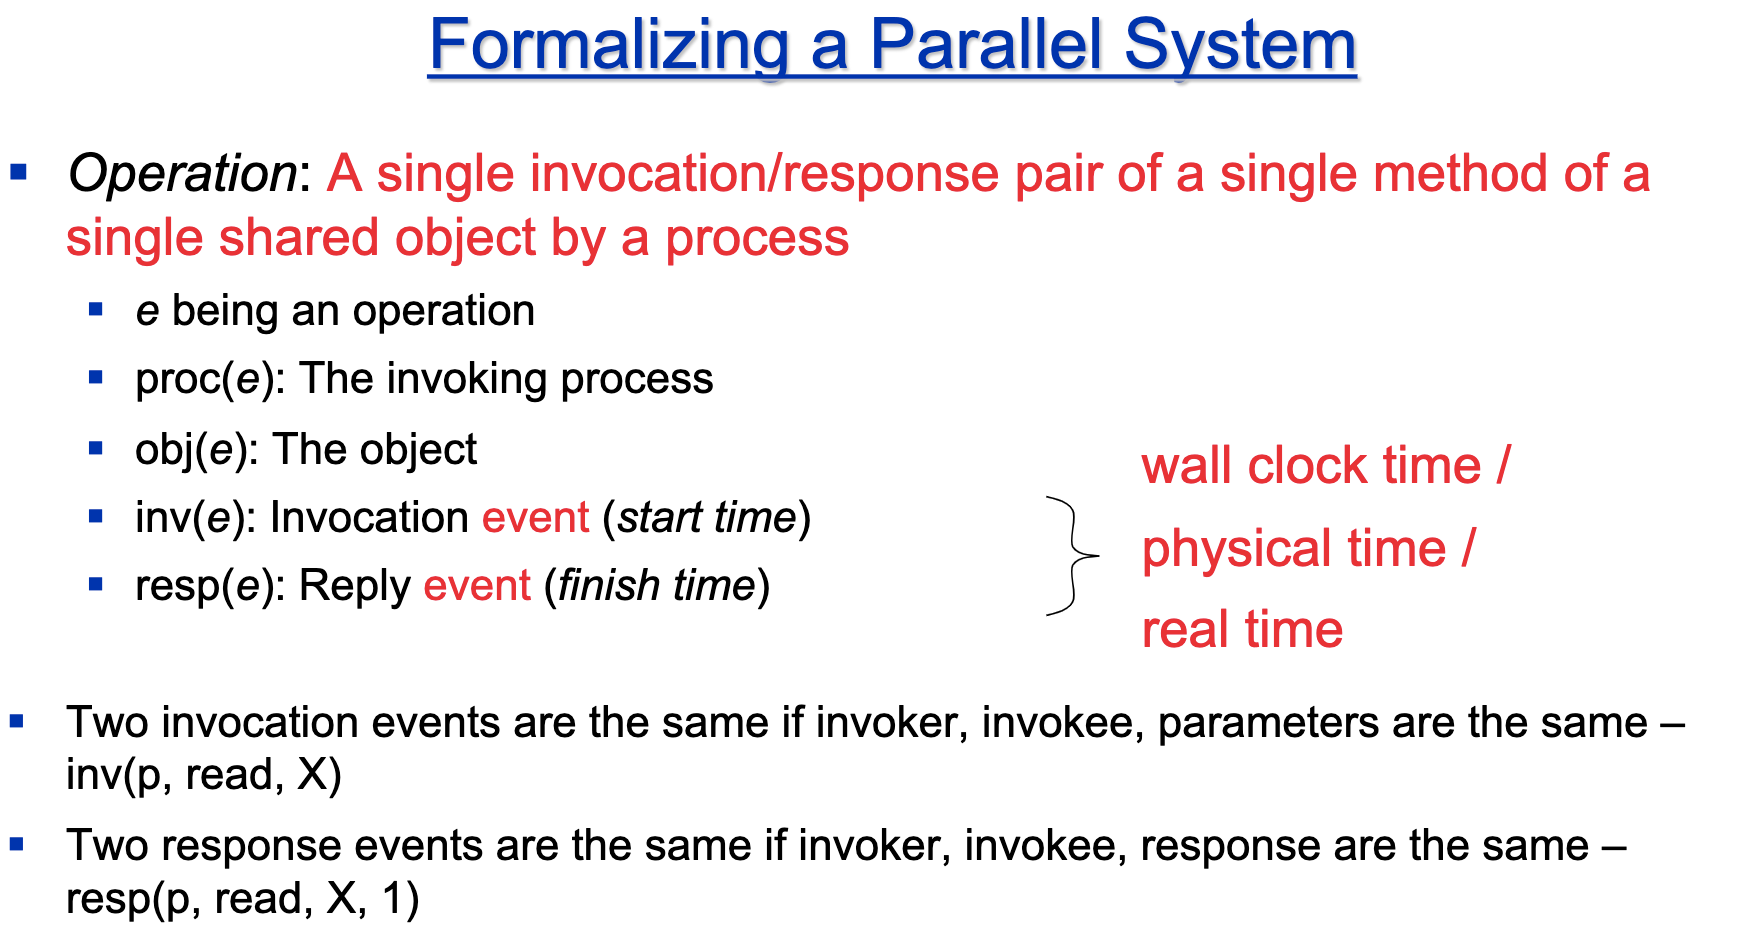
\includegraphics[width=0.8\linewidth]{cs4231-formalising-parallel-system.png} 
  \end{tightcenter}

  \begin{itemize}
    \item \definition{consistency} specifies what behaviour is allowed when a shared object is accessed by multiple processes
      \begin{itemize}
        \item “consistent” = satisfies the specification
      \end{itemize}
    \item \definition[$H$]{history} a sequence of invocations and responses ordered by wall clock time
      \begin{itemize}
        \item for any invocation $H$, the corresponding response must be in $H$
        \item each execution of a parallel system corresponds to a history and vice versa
      \end{itemize}
    \item \definition{sequential} an invocation is always \textit{immediately} followed by its response 
      \begin{itemize}
        \item no interleaving (else is \ildefinition{concurrent})
          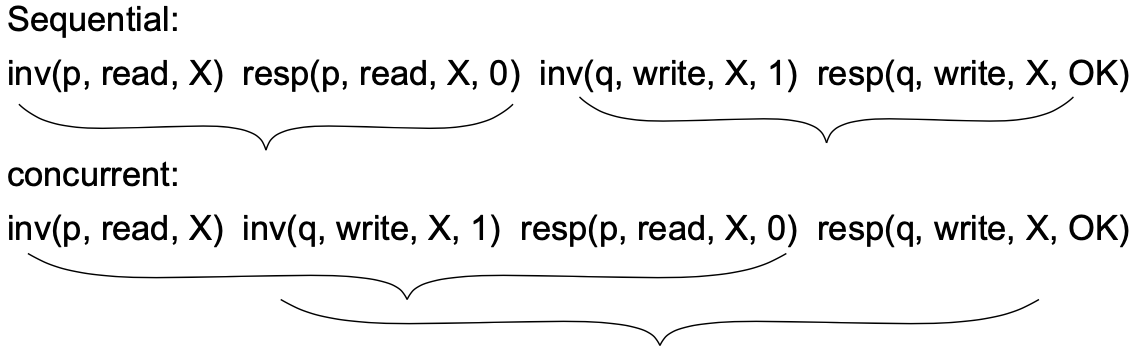
\includegraphics[width=0.7\linewidth]{cs4231-sequential-concurrent.png} 
      \end{itemize}
    \item a history H is \definition{legal} if all responses satisfies the sequential semantics of the data type
      \begin{itemize}
        \item \definition{sequential semantics} the semantics you would get if there is \textit{only one process} accessing that data type
        \item possible for sequential history to not be legal
          \begin{itemize}
            \item e.g. x=0, P1 writes 1 to x, P2 reads 0 from x (if it were the same thread it would have been the same value)
          \end{itemize}
      \end{itemize}
    \item process $p$’s \definition[of $H$, $H | p$]{process subhistory} the subsequence of all events of p
      \begin{itemize}
        \item process subhistory is always sequential
      \end{itemize}
    \item object $o$'s \definition[of $H$, $H \vert o$]{object subhistory} the subsequence of all events of $o$
    \item two histories are \definition{equivalent} if they have the exact same set of events
      \begin{itemize}
        \item same events $\Rightarrow$ implies all responses are the same
        \item may be different ordering of events (only care about responses)
      \end{itemize}
    \item \definition{process/program order} a partial order among all events
      \begin{itemize}
        \item within the same process, process order is the same as execution order
        \item no other additional orderings
      \end{itemize}
    \item \definition{sequential consistency} equivalent to some legal sequential history that preserves process order
      \begin{itemize}
        \item \textit{(Lamport’s definition)} results are same as in some sequential order \& preserves program order
      \end{itemize}
  \end{itemize}

  \subsection{Linearisability}

  \begin{itemize}
    \item stronger than sequential consistency
    \item \definition{external order} a history H induces the “<” partial order among operations
      \begin{itemize}
        \item $o1 < o2 \iff$ the response of o1 appears in H before the invocation of o2
          \begin{itemize}
            \item aka o1 finishes before o2 starts
          \end{itemize}
        \item preserves external order $\Rightarrow$ preserves program order
      \end{itemize}
    \item \definition{linearisability} sequentially consistent (with some legal sequential history S) and S preserves the external order in H
      \begin{itemize}
        \item \textit{(alternate definition)} The execution is equivalent to some execution such that each operation happens instantaneously at some point between the invocation and response
          \begin{itemize}
            \item for every operation in the execution, you can find a linearisation point between the invocation and response event
          \end{itemize}
        \item linearisable $\Rightarrow$ sequentially consistent
      \end{itemize}
  \end{itemize}

  \subsubsection{local property}

  \begin{itemize}
    \item linearisability is a local property
      \begin{itemize}
        \item H is linearisable $\iff$ for any object x, $H \vert x$ is linearisable
        \item useful because you can reason about objects instead
      \end{itemize}
    \item sequential consistency is not a local property
      \begin{itemize}
        \item H may not be sequentially consistent, but H|x and H|y can be sequentially consistent
      \end{itemize}
  \end{itemize}
  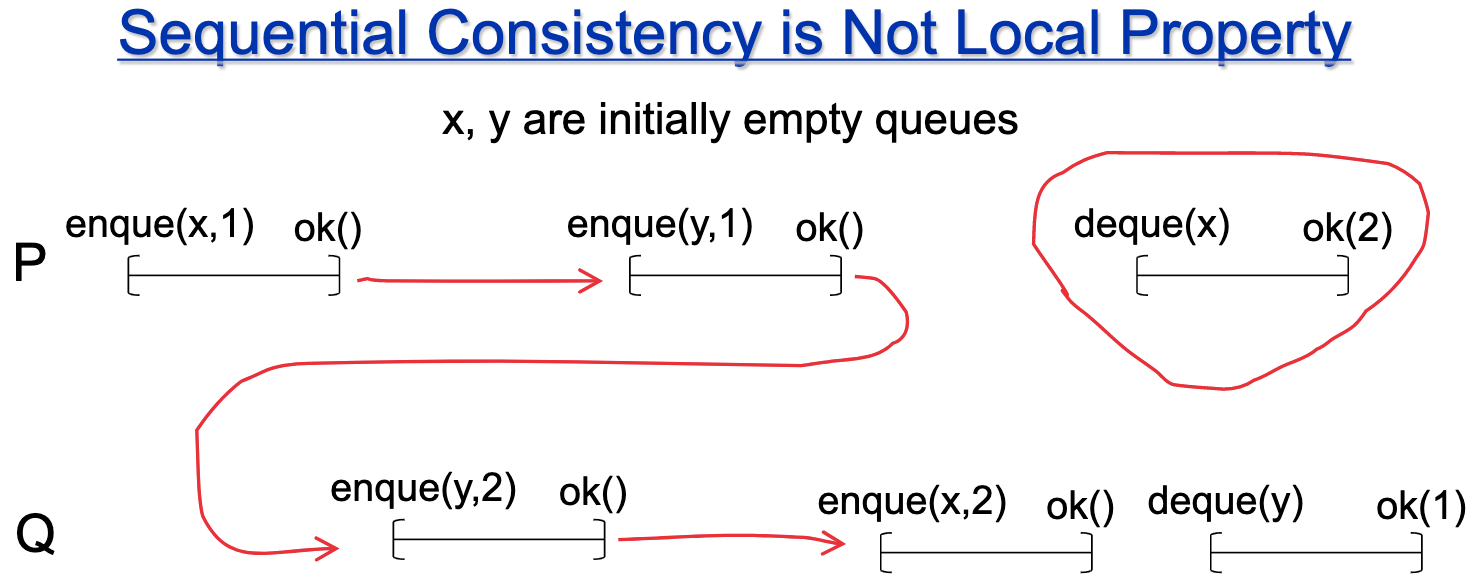
\includegraphics[width=0.65\linewidth]{cs4231-sequential-consistency-not-local.png} 
  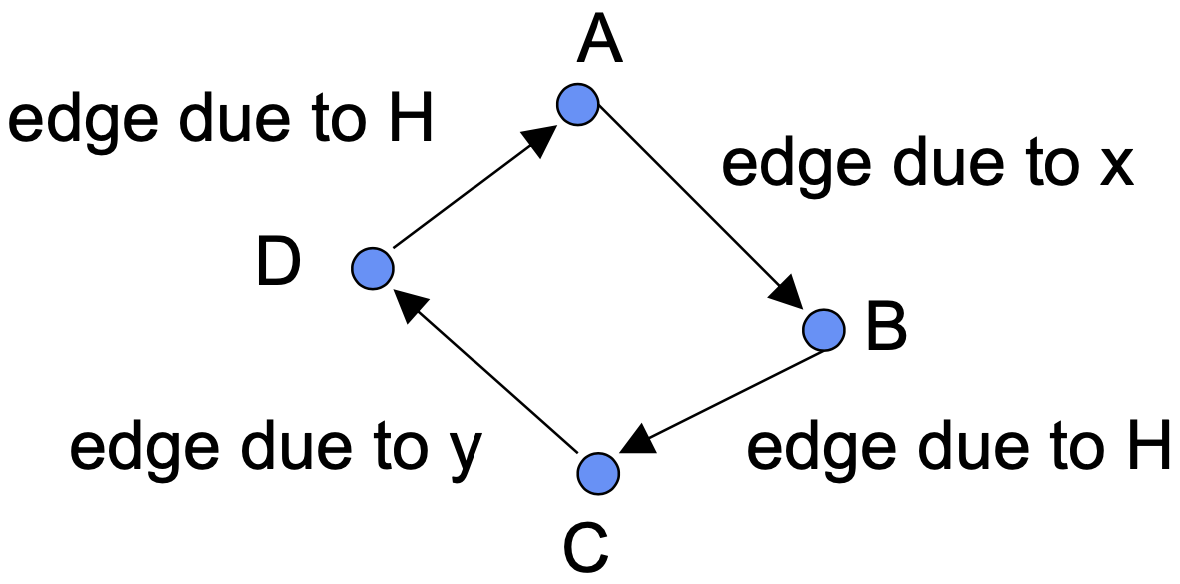
\includegraphics[width=0.3\linewidth]{cs4231-linearisability-local-property-proof.png} 

  \textbf{proof: linearisability is a local property}

  \begin{itemize}
    \item using a directed graph: directed edge from $o1 \rightarrow o2$ if
      \begin{itemize}
        \item $o1$ and $o2$ are on the same object $x$ and $o1$ is before $o2$ when linearising $H \vert x$ \\* ($o1\rightarrow o2$ due to obj)
        \item $o1 < o2$ in external order ($o1\rightarrow o2$ due to $H$)
      \end{itemize}
    \item any topological sorting of the graph gives us a legal sequential history S
    \item any cycle must be composed of
      \begin{itemize}
        \item edges to some object $x$ ($\approx 1$ edge since H|x is equivalent S with a total order)
        \item edges due to some H ($\approx 1$ edge since partial order induced by H is transitive)
        \item edges due to some object $y$ ($\approx 1$ edge)
        \item edges due to some H ($\approx 1$ edge)
      \end{itemize}
  \end{itemize}

  \subsection{Consistency definitions for registers}

  \begin{itemize}
    \item \definition{register} ADT: a single value that can be read and written
      \begin{itemize}
        \item \definition{atomic} if the implementation always ensures linearisability of the history
        \item \definition{sequentially consistent} if the implementation always ensures sequential consistency of the history
        \item \definition{regular} when a read
          \begin{itemize}
            \item not overlap with any write, the read returns the value written by one of the most recent writes
            \item overlaps with one or more writes, the read returns the value written by one of the most recent writes OR the value written by one of the overlapping writes
              \\* 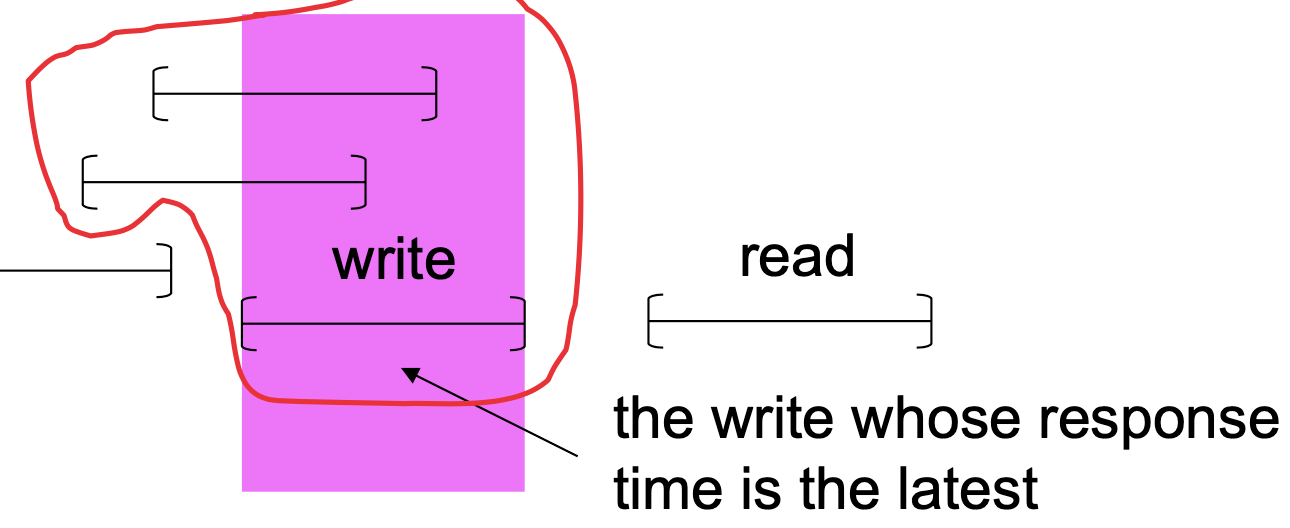
\includegraphics[width=0.5\linewidth]{cs4231-register-recent-writes.png} 
          \end{itemize}
        \item \definition{safe} if the implementation always ensures that
          \begin{itemize}
            \item when a read does not overlap with any write, it returns the value written by one of the most recent writes
            \item when a read overlaps with one or more writes, it can return anything
          \end{itemize}
      \end{itemize}
    \item \attention atomic $\Rightarrow$ regular $\Rightarrow$ safe
    \item regular $\not\Rightarrow$ sequentially consistent; $\quad$ sequentially consistent $\not\Rightarrow$ regular
      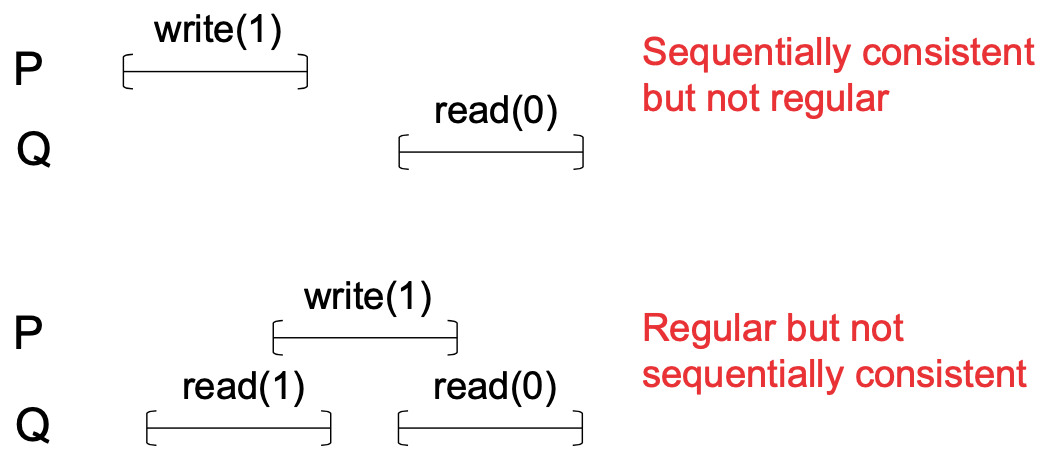
\includegraphics[width=0.6\linewidth]{cs4231-register-regular-seq-consistent.png} 
  \end{itemize}

  \vfill\null
  \columnbreak

  \section{04. MODELS \& CLOCKS}

  \begin{itemize}
    \item process can perform 3 kinds of atomic events/actions
      \begin{itemize}
        \item \textbf{local computation}
        \item \textbf{send} a single message to a single process
        \item \textbf{receive} a single message from a single process
      \end{itemize}
    \item \textbf{communication model}
      \begin{itemize}
        \item point-to-point (to send to multiple processes: multiple send events)
        \item error-free, infinite buffer
        \item potentially out of order
      \end{itemize}
    \item \textbf{software clocks} 
      \begin{itemize}
        \item capture event ordering that are visible to users who do not have physical clocks
        \item allows a protocol to infer ordering among events
      \end{itemize}
  \end{itemize}

  \subsubsection{visible orderings}

  \begin{itemize}
    \item \definition{process order} if A and B are on the same process, I can tell that A is before B
    \item \definition{send-receive order} the send event must be before the receive event
    \item \definition{transitivity} if A<B and B<C, then A<C
  \end{itemize}

  \begin{tightcenter}
    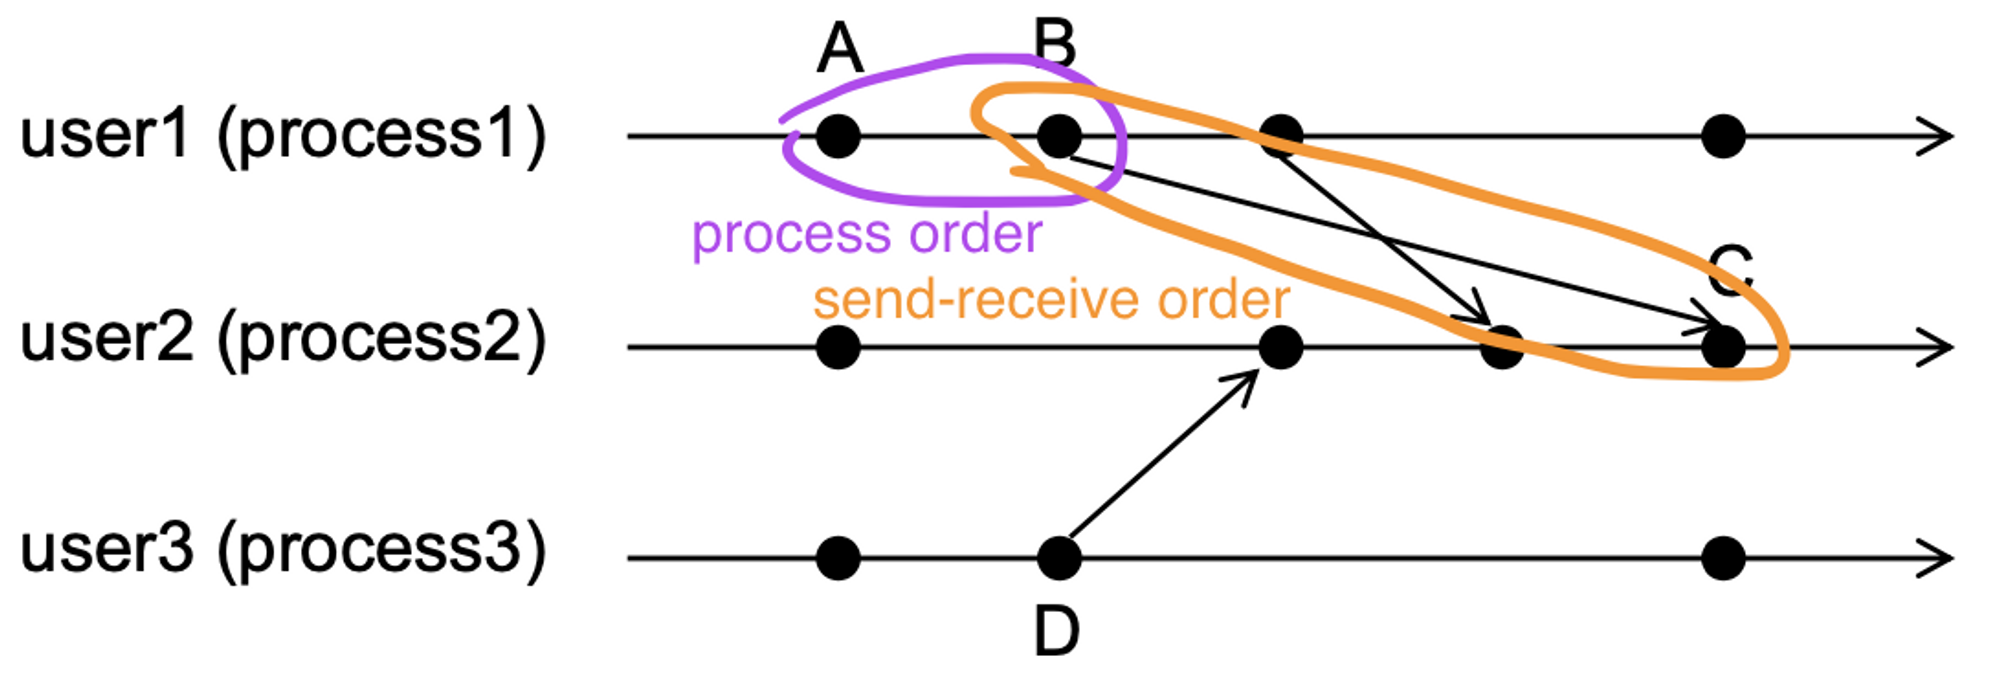
\includegraphics[width=0.7\linewidth]{cs4231-visible-orderings.png} 
  \end{tightcenter}

  \begin{itemize}
    \item \ildefinition{happened-before} relation (denoted \ildefinition{$e\rightarrow f$}) captures the ordering that is visible to users when there is no physical clock
      \begin{itemize}
        \item partial order among events
      \end{itemize}
    \item \ildefinition{concurrent-with} relation (denoted \ildefinition{$e \vert \vert f$}) if $\quad \lnot (e \rightarrow f) \land \lnot(f \rightarrow e)$
  \end{itemize}

  \subsection{Logical Clocks}

  \begin{itemize}
    \item each event has a single integer as its logical clock value
    \item each process has a local counter $C$
    \item protocol
      \begin{itemize}
        \item increment $C$ at each \textbf{local computation} and \textbf{send event}
        \item \textbf{send event:} attaches the logical clock value $V$ to the message
        \item \textbf{receive event:} $C = \max(C, V)+1$
      \end{itemize}
    \item if event $s$ happens before event $t$ $\Rightarrow$ $C_s < C_t$
      \begin{itemize}
        \item $C_s < C_t \not\Rightarrow s$ happens before $t$
          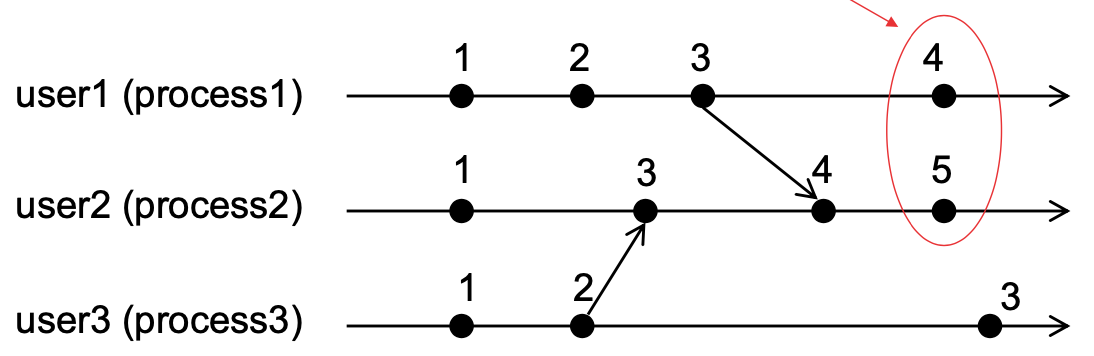
\includegraphics[width=0.6\linewidth]{cs4231-logical-clocks-happens-before-counterexample.png} 
      \end{itemize}
    \item for total order, extend with process number
      \begin{itemize}
        \item $s.c$ denotes the value of $c$ in state $s$, $s.p$ indicates the process it belongs to
        \item the timestamp of any event is a tuple $(s.c, s.p)$
        \item $(s.c, s.p) < (t.c, t.p) \iff (s.c < t.c) \lor ((s.c = t.c) \land (s.p < t.p))$
      \end{itemize}
  \end{itemize}

  \subsection{Vector Clocks}

  \begin{itemize}
    \item event $s$ happens-before event $t$ $\iff$ $C_s < C_t$
    \item  each event has a vector of $n$ integers as its vector clock value
      \begin{itemize}
        \item $v1=v2$ if all $n$ fields are the same
        \item $v1 \leq v2$ if every field in $v1$ is less than or equal to the corresponding field in $v2$
          \begin{itemize}
            \item e.g. (3,1,5)$\leq$(4,1,7)
          \end{itemize}
        \item $v1<v2$ if $v1 \leq v2$ and $v1 \neq v2$ $\quad\quad$ (< is NOT a total order here)
      \end{itemize}
    \item each process $i$ has a local vector $C$
    \item protocol
      \begin{itemize}
        \item increment C[i] at each \textbf{local computation} and \textbf{send} event
          \begin{itemize}
            \item $i^{th}$ entry is the principle entry
            \item process $i$ is the only process that can create new values for the $i^{th}$ entry
          \end{itemize}
        \item \textbf{send event:} vector clock value $V$ is attached to the message
        \item \textbf{receive event:} $C= \pairwisemax(C,V)$ \texttt{; C++}
      \end{itemize}
  \end{itemize}

  \begin{tightcenter}
    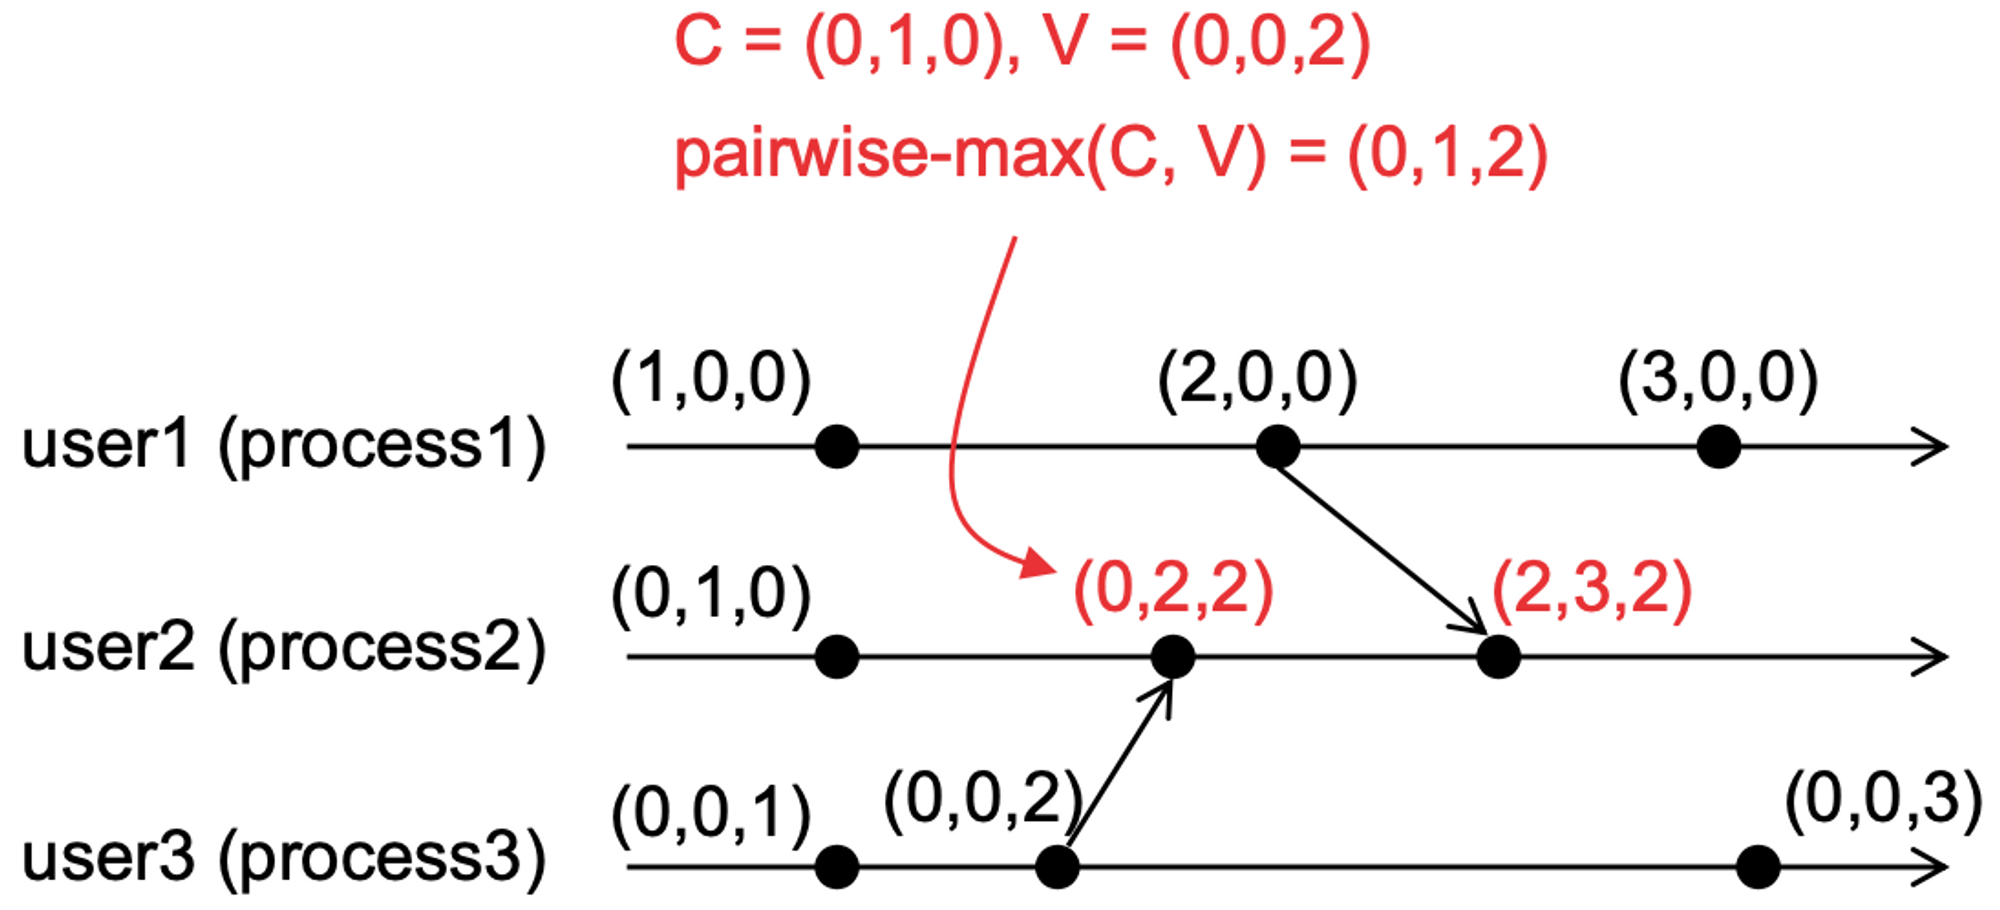
\includegraphics[width=0.5\linewidth]{cs4231-vector-clocks.png} 
  \end{tightcenter}

  \subsection{Matrix Clocks}

  \begin{itemize}
    \item each event has 1 vector clock for each process
      \begin{itemize}
        \item the $i^{th}$ process on vector $i$ is called process $i$’s principle vector
      \end{itemize}
    \item protocol
      \begin{itemize}
        \item for \textit{principal vector} $C$ on process $i$,
          \begin{itemize}
            \item increment C[i] at each \textbf{local computation} and \textbf{send} event
            \item \textbf{send event:} all $n$ vectors are attached to the message
            \item \textbf{receive event:}  $C= \pairwisemax(C,V)$ \texttt{; C[i]++}
              \begin{itemize}
                \item where $V$ is the principle vector of the sender
              \end{itemize}
          \end{itemize}
        \item for \textit{non-principal vector} $C$ on process $i$
          \begin{itemize}
            \item \textbf{receive event:} $C= \pairwisemax(C,V)$;
          \end{itemize}
      \end{itemize}
  \end{itemize}

  \begin{tightcenter}
    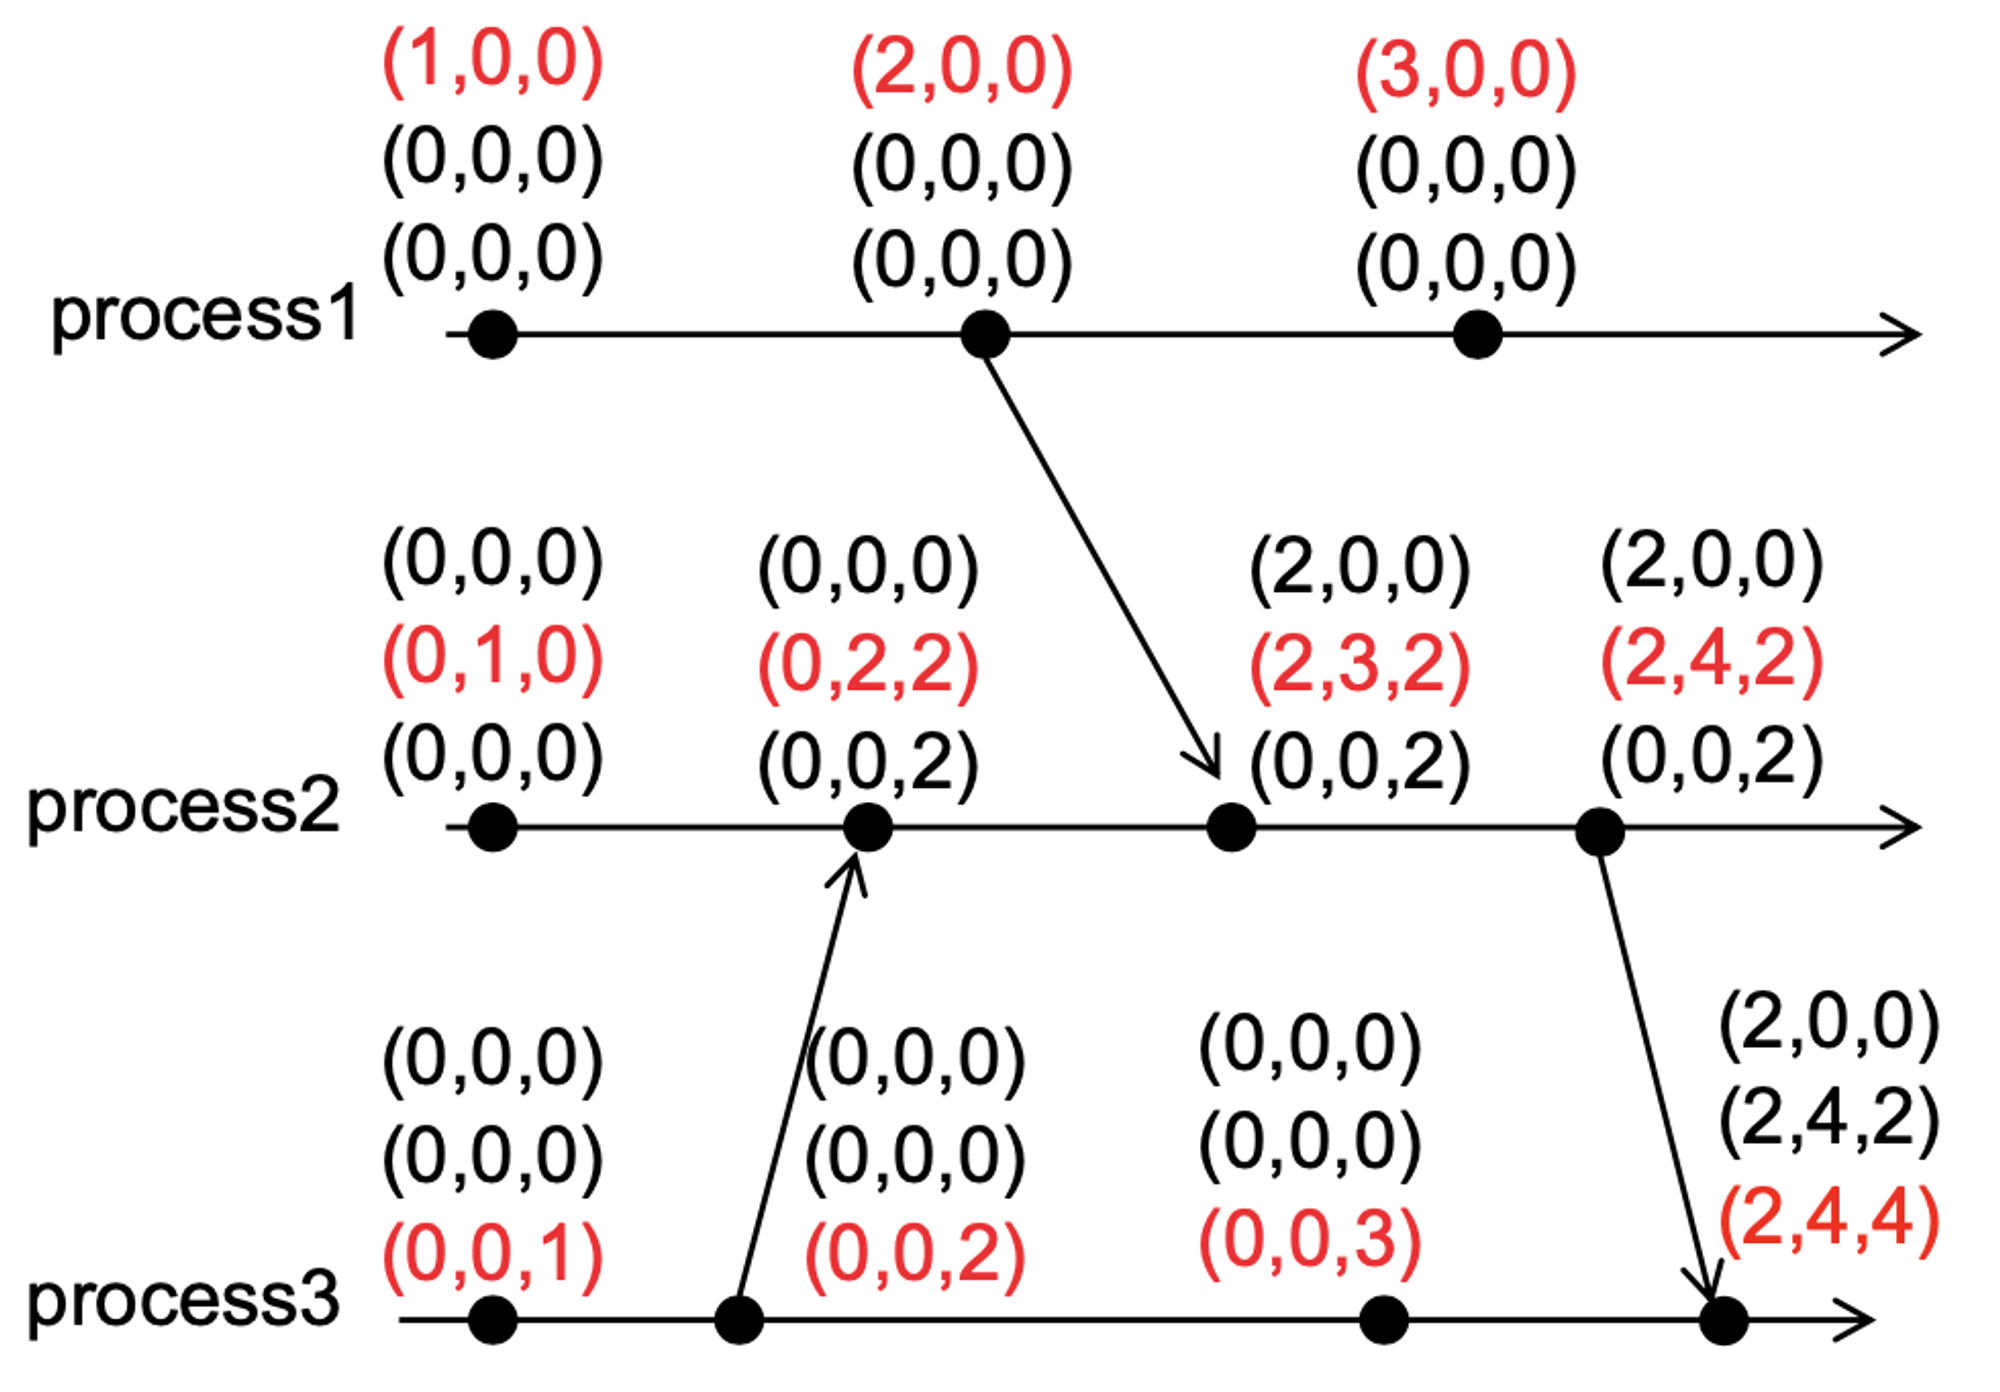
\includegraphics[width=0.6\linewidth]{cs4231-matrix-clock.png} 
  \end{tightcenter}

  \vfill\null
  \columnbreak

  \section{05. GLOBAL SNAPSHOT}

  \begin{itemize}
    \item captures a snapshot of local states on n processes such that the global snapshot could have happened sometime in the past (user cannot tell the difference)
  \end{itemize}

  \subsection{Consistent Snapshot}

  \begin{itemize}
    \item \definition{consistent snapshot} a snapshot of local states on n processes such that the global snapshot could have happened sometime in the past 
      \begin{itemize}
        \item can have outgoing (L $\rightarrow$ R) arrows, but can’t have incoming (R $\rightarrow$ L) arrows
      \end{itemize}
  \end{itemize}
  \begin{tightcenter}
    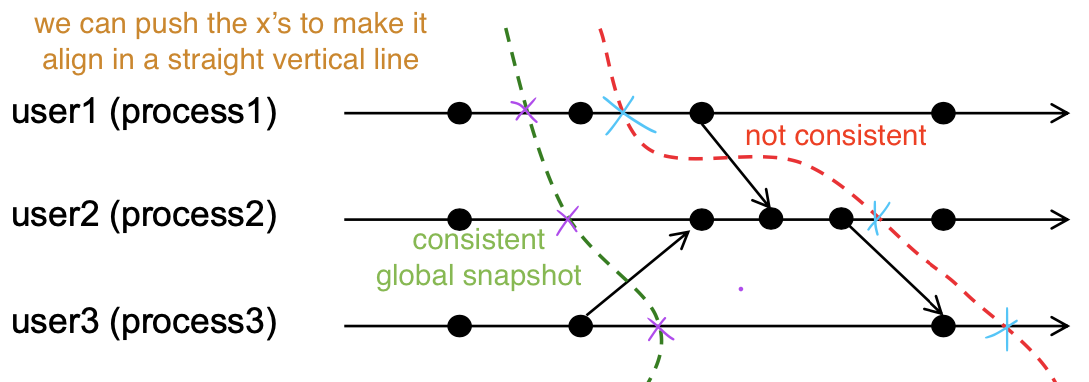
\includegraphics[width=0.7\linewidth]{cs4231-consistent-snapshot.png} 
  \end{tightcenter}

  \begin{itemize}
    \item \definition{global snapshot} a set of events such that if $e2$ is in the set and $e1$ is before $e2$ in process order, then $e1$ must be in the set
      \begin{itemize}
        \item a collection of local snapshots
      \end{itemize}
    \item \definition{consistent local snapshot} a global snapshot s.t. if $e2$ is in the set and $e1$ is before $e2$ in send-receive order, then $e1$ must be in the set
      \begin{itemize}
        \item aka global snapshot + any receive event in the set has its corresponding send event in the set 
        \item transitive relations implied
      \end{itemize}
  \end{itemize}
  \begin{tightcenter}
    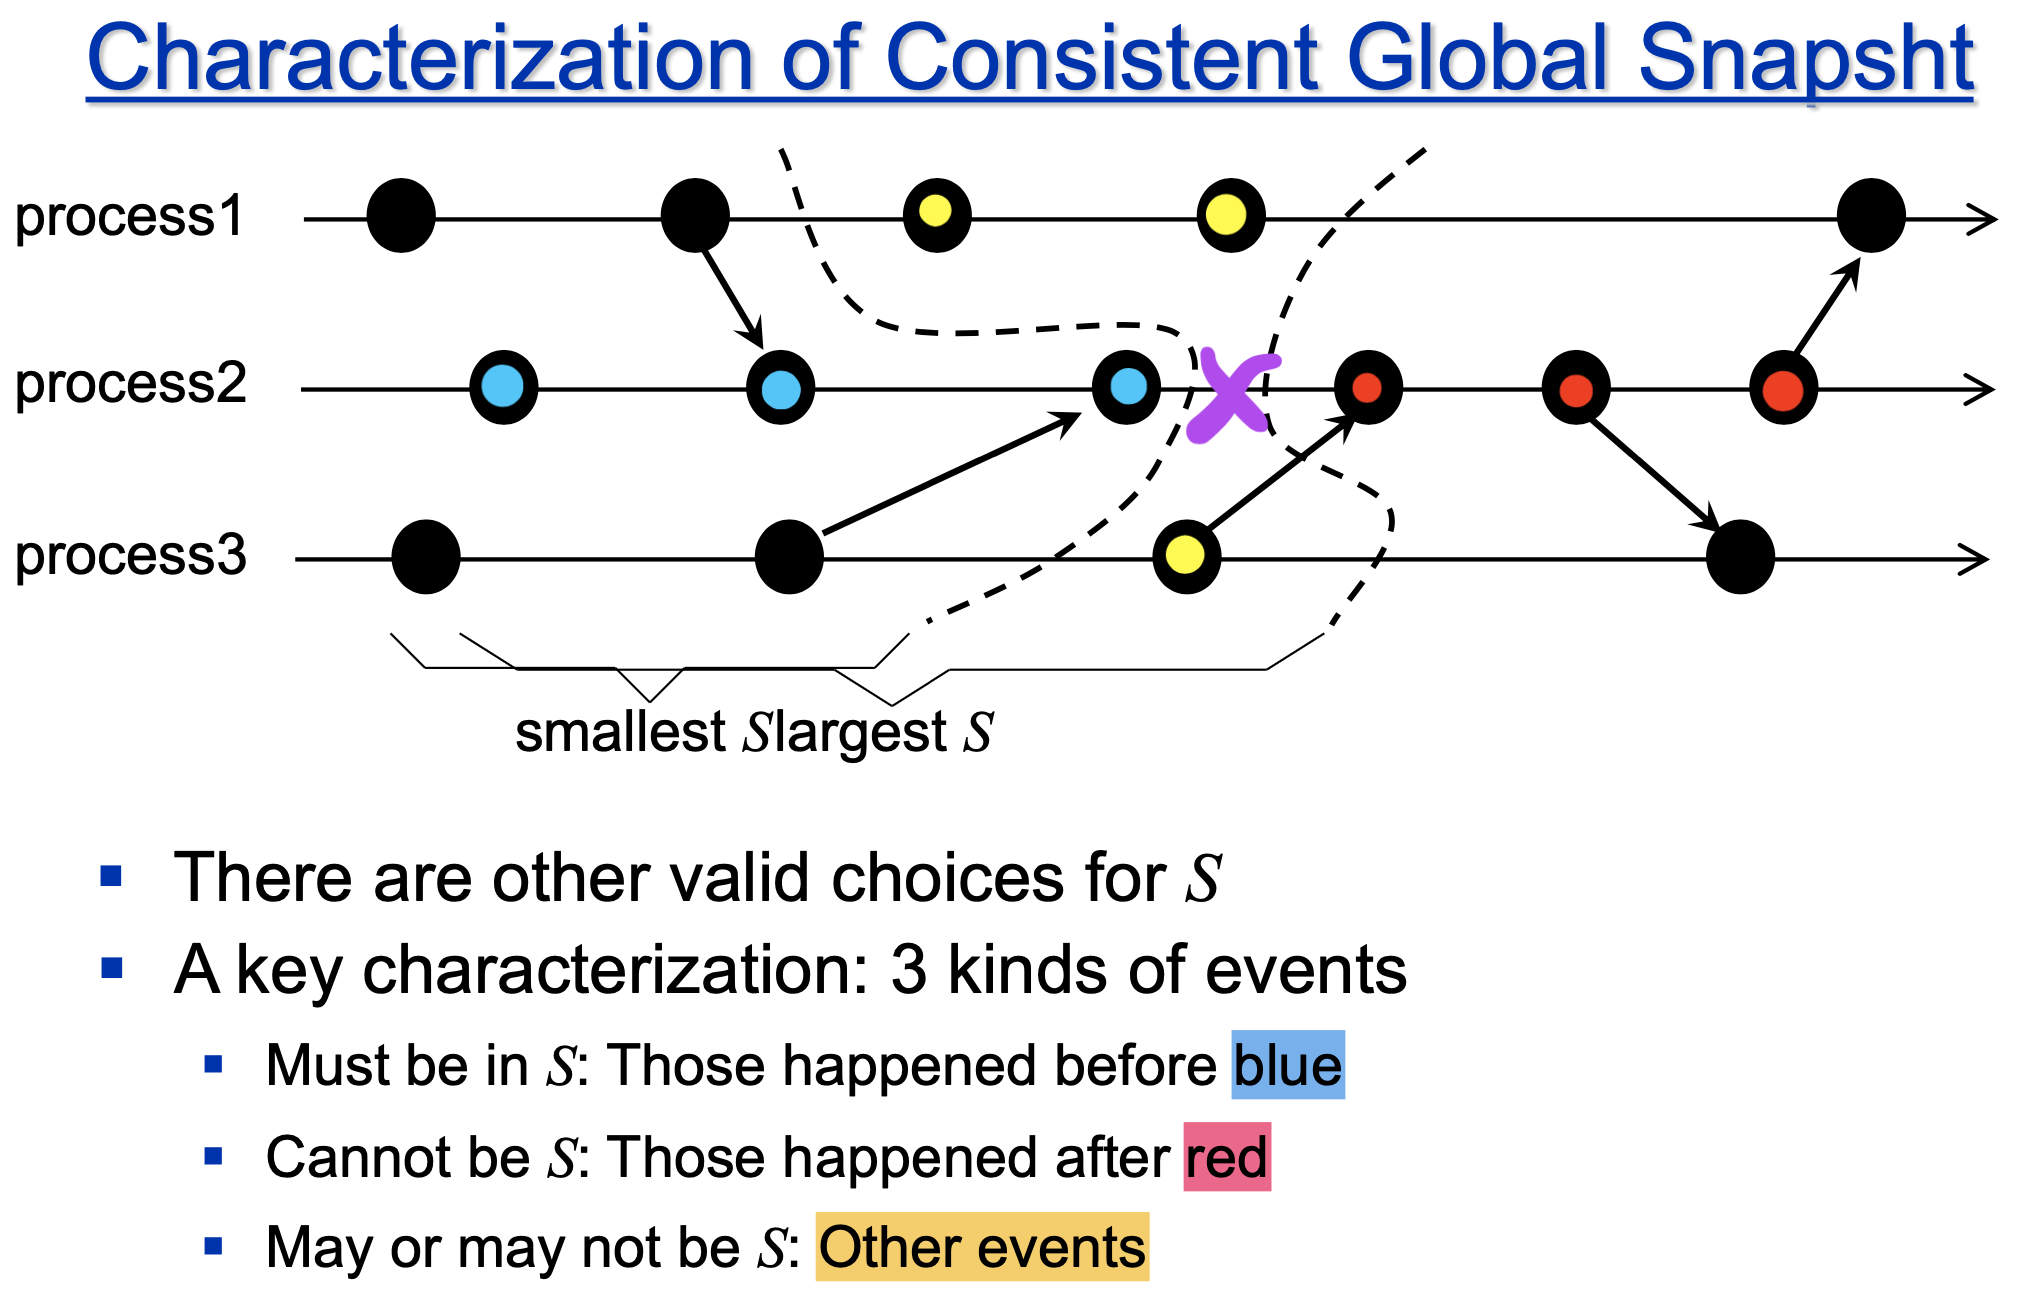
\includegraphics[width=0.6\linewidth]{cs4231-consistent-global-snapshot.png} 
  \end{tightcenter}

  \subsubsection{capturing a CGS}

  \begin{itemize}
    \item communication model
      \begin{itemize}
        \item no message loss
        \item communication channels are unidirectional (model bidirectional channels as 2 unidirectional channels)
        \item FIFO delivery on each channel
      \end{itemize}
    \item ensuring FIFO
      \begin{itemize}
        \item each process maintains a message number counter for each channel and stamps each message sent
        \item receiver will only deliver messages in order
      \end{itemize}
  \end{itemize}

  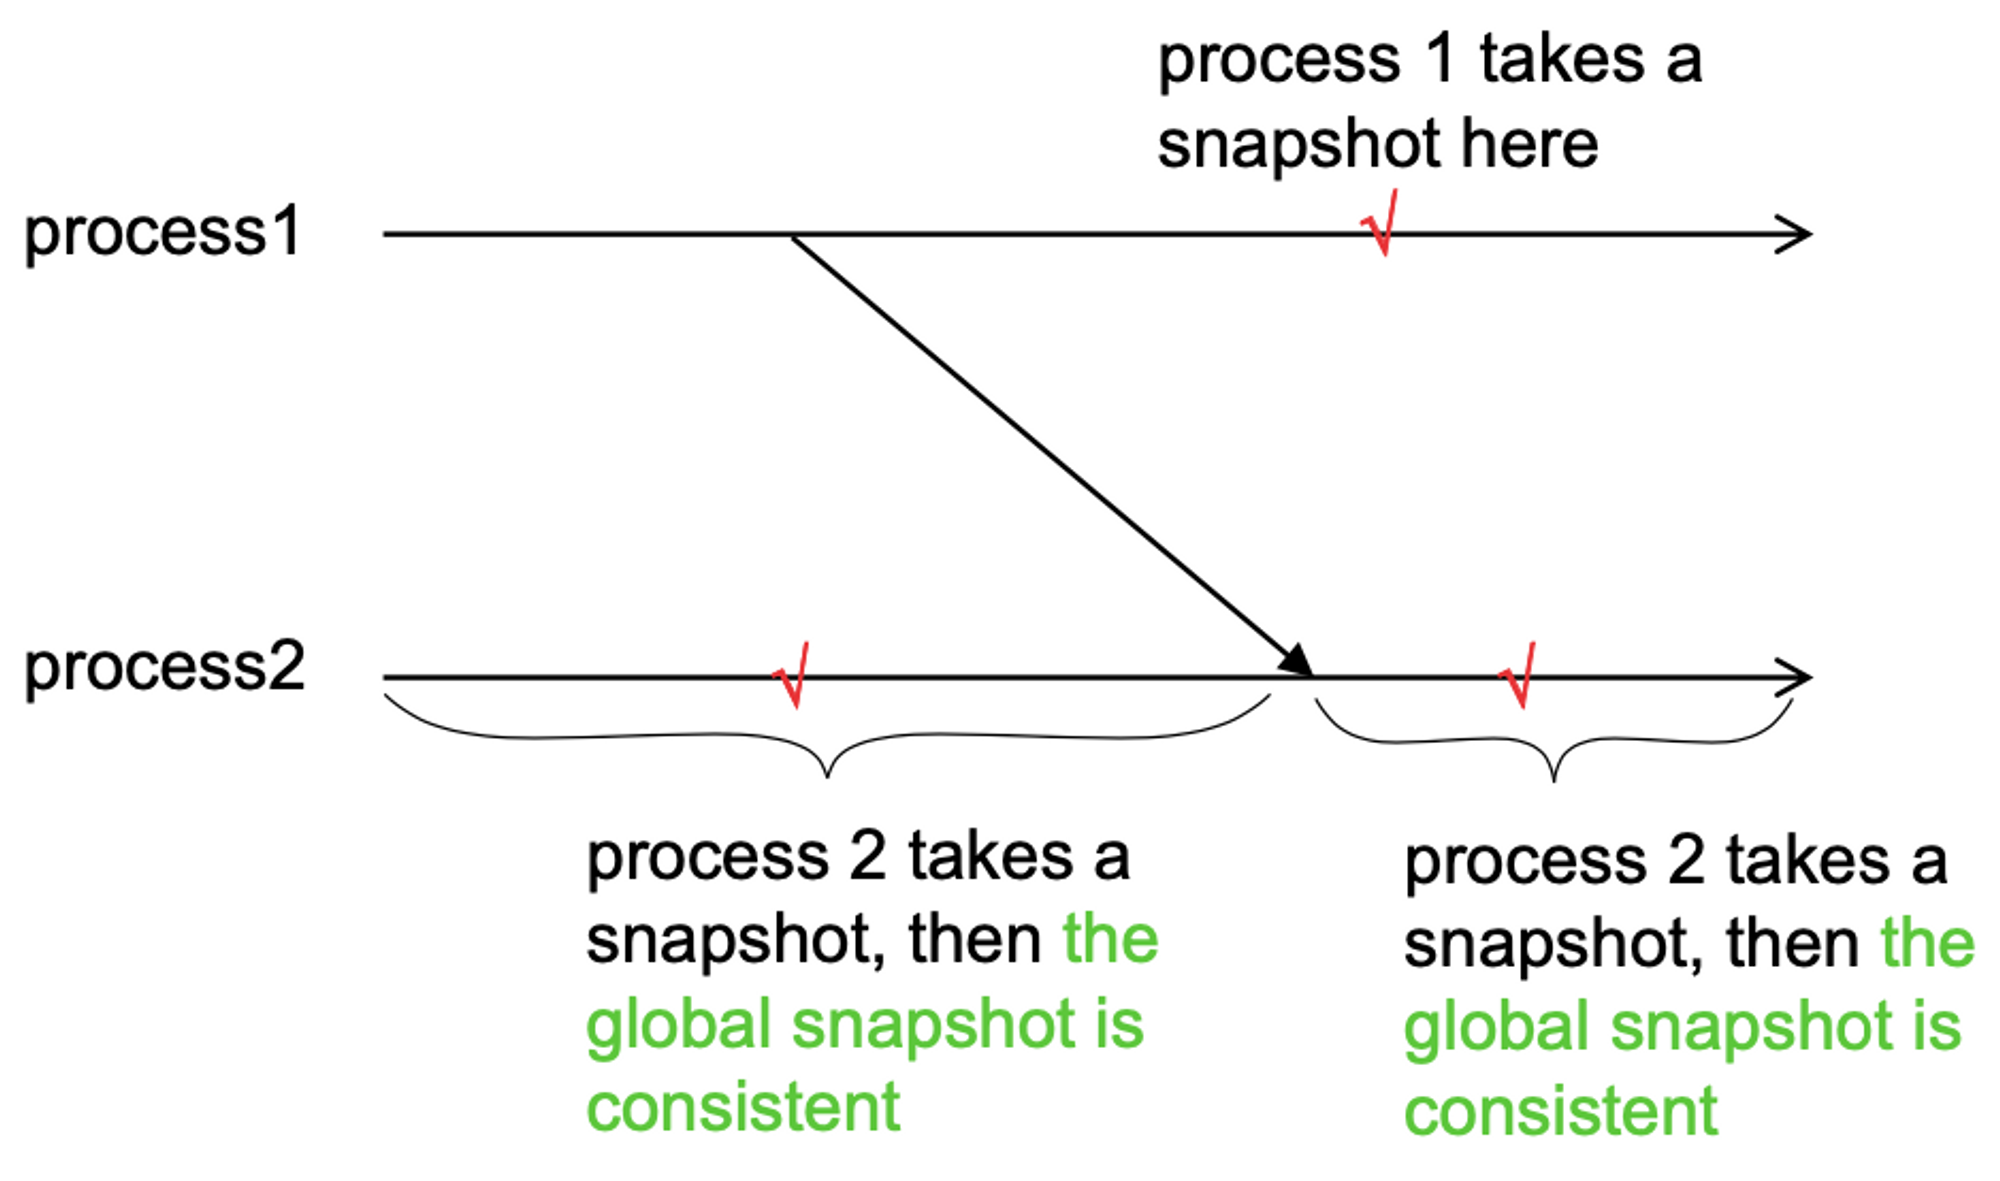
\includegraphics[width=0.48\linewidth]{cs4231-cgs-1.png} 
  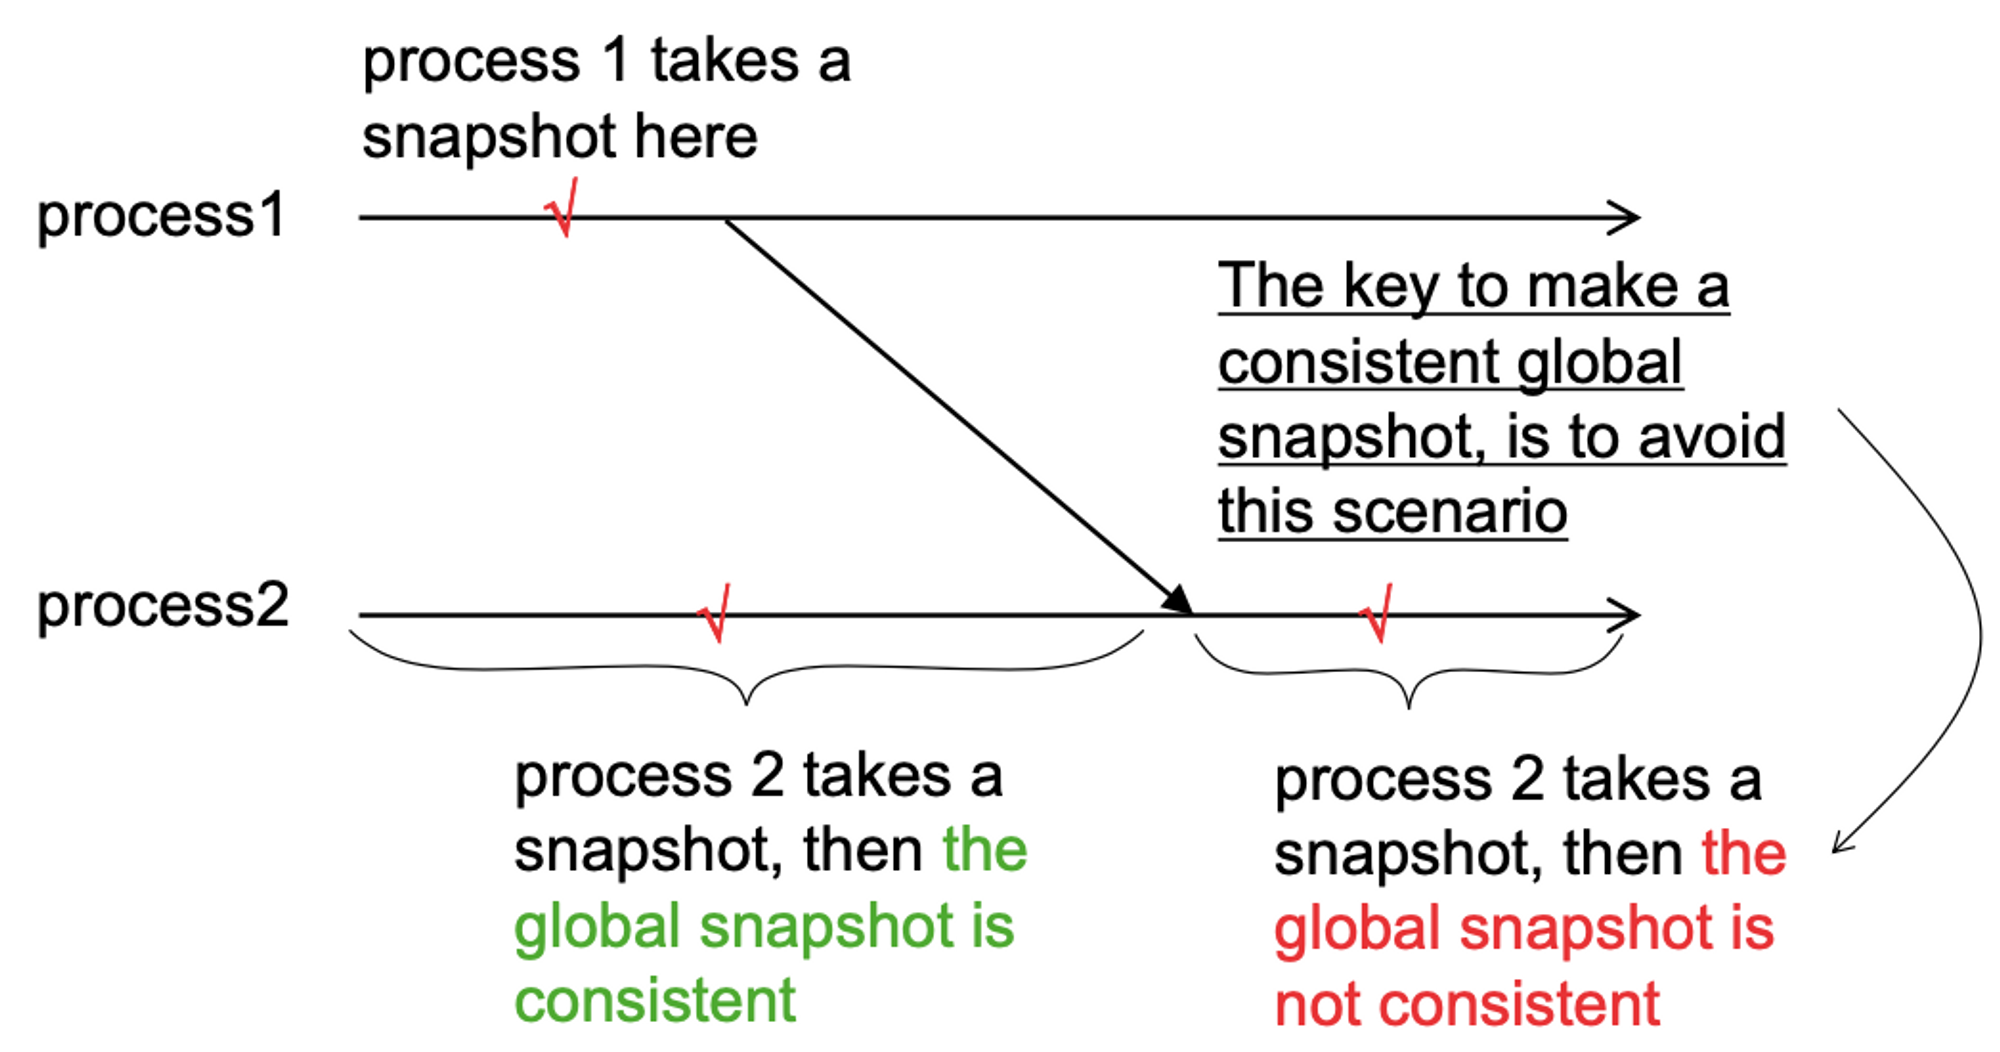
\includegraphics[width=0.48\linewidth]{cs4231-cgs-2.png} 

  \subsubsection{Chandy \& Lamport's Protocol}

  \begin{itemize}
    \item each process is either
      \begin{itemize}
        \item red - has taken local snapshot
        \item white - has not taken local snapshot
      \end{itemize}
    \item protocol initiated by a single process by turning itself from white to red
      \begin{itemize}
        \item once a process turns red, immediately send out Marker messages to all other processes
        \item upon receiving Marker, process turns red
        \item total $n*(n-1)$ Marker messages
      \end{itemize}
    \item requires FIFO - marker messages are sent on the same channel as actual messages
    \item \textbf{on-the-fly} messages: sent before sender's local snapshot, received after receiver's local snapshot
  \end{itemize}
  \begin{tightcenter}
    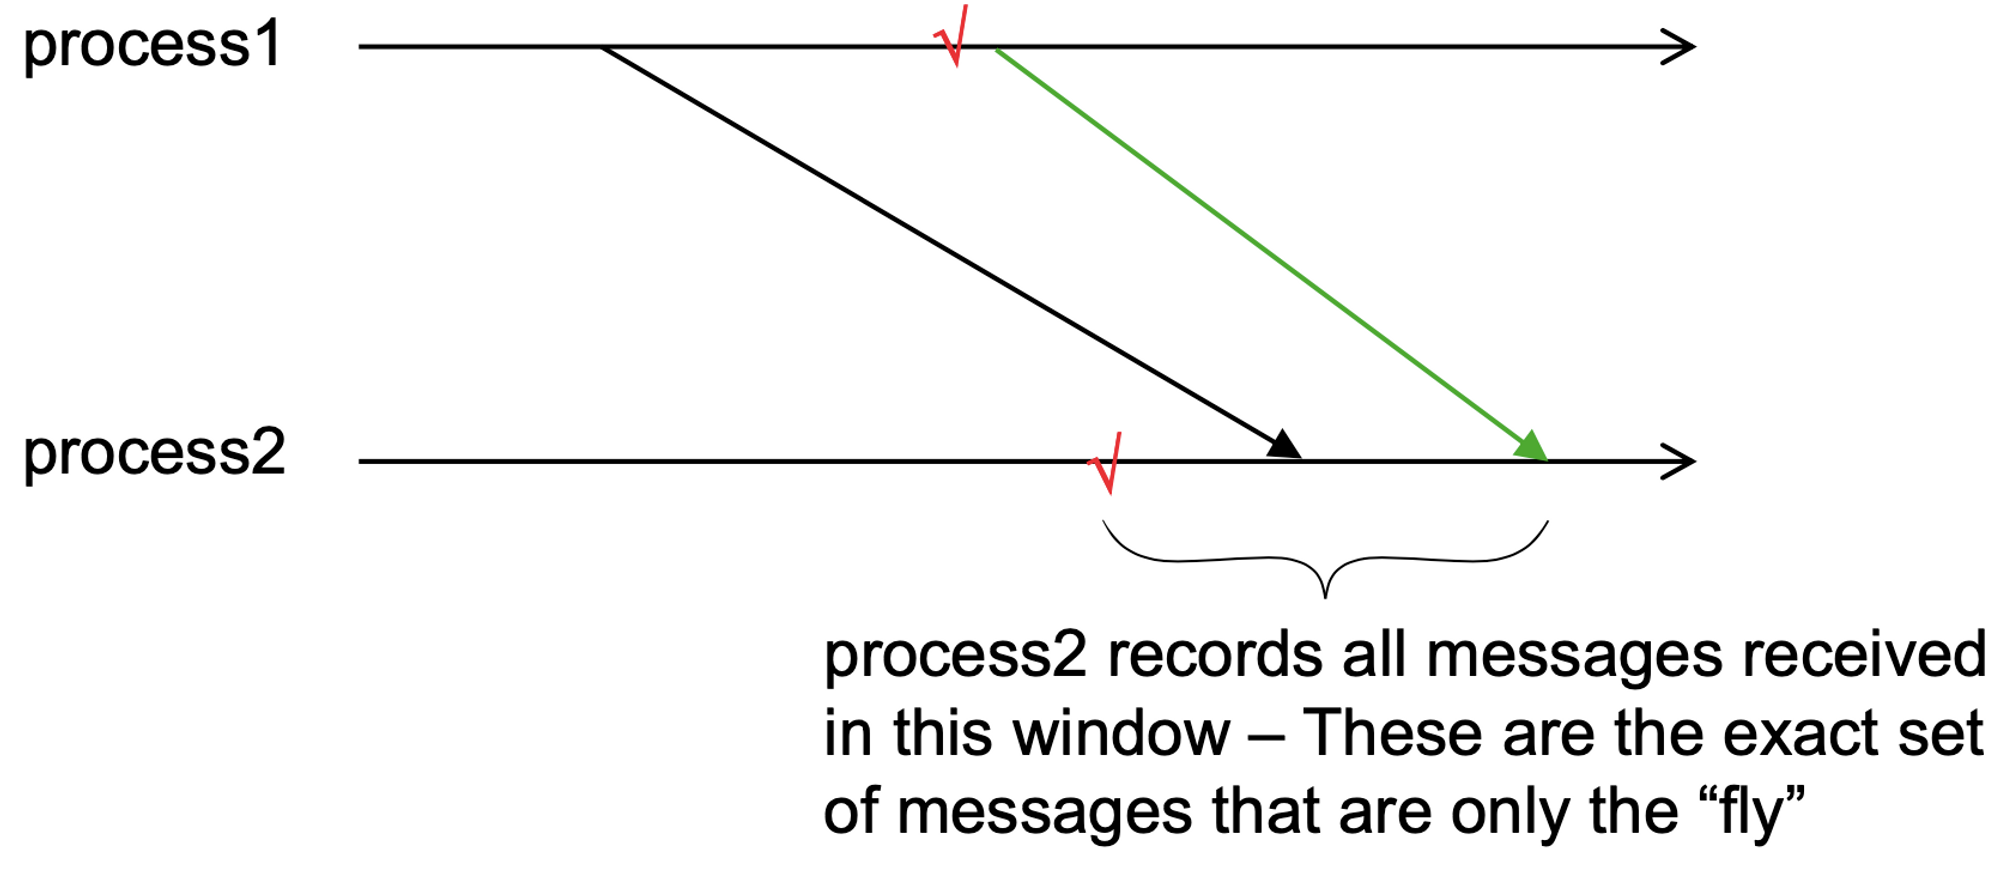
\includegraphics[width=0.6\linewidth]{cs4231-cgs-onthefly.png} 
  \end{tightcenter}

  \vfill\null
  \columnbreak

  \section{06. MESSAGE ORDERING}

  \subsection{Causal Order}

  \begin{itemize}
    \item \definition{causal order} if $s1$ happened before $s2$, and $r1$ and $r2$ are on the same process, then $r1$ must be before $r2$
      \begin{itemize}
        \item $s_1 \rightarrow s_2 \Rightarrow \lnot(r_2 \prec r_1)$
      \end{itemize}
    \item \definition{FIFO} any 2 messages from process $P_i$ to $P_j$ are received in the same order as they are sent
      \begin{itemize}
        \item $s_i \prec s_j \Rightarrow \lnot(r_j \prec r_i)$
      \end{itemize}
    \item \ildefinition{$e \prec f$}  denotes $e$ occurred before $f$ in the same process
    \item \ildefinition{$s_i\leadsto r_i$}  denotes $s_i$ is the send event corresponding to receive event $r_i$
  \end{itemize}

  \subsubsection{protocol: ensure causal order}

  \begin{itemize}
    \item each process maintains a $n$ by $n$ matrix $M$
      \begin{itemize}
        \item $M[i, j]$ = \# of messages sent from $i$ to $j$, as known by local (current) process
      \end{itemize}
    \item when process $i$ sends a message to process $j$,
      \begin{itemize}
        \item on process $i$:  $M[i, j]\texttt{++}$
        \item piggyback $M$ on the message
      \end{itemize}
    \item when process $j$ (with local matrix $M$) receives a message from process $i$ with matrix $T$ piggybacked,
      \begin{itemize}
        \item set $M = \pairwisemax(M, T)$ if $\begin{cases} T[k, j]\leq M[k, j] \quad \text{for all }k\neq i\\ T[i, j] = M[i, j] + 1 \end{cases}$
          \begin{itemize}
            \item intuition: $M[i, j]$ on process $j$ takes on consecutive values
            \item if the entry is >1 larger than the local entry, it means that there is another message in propagation
              \begin{itemize}
                \item we only care about column $j$ - [i, j] should have a difference of 1
              \end{itemize}
          \end{itemize}
        \item else, delay the message
      \end{itemize}
      \begin{tightcenter}
        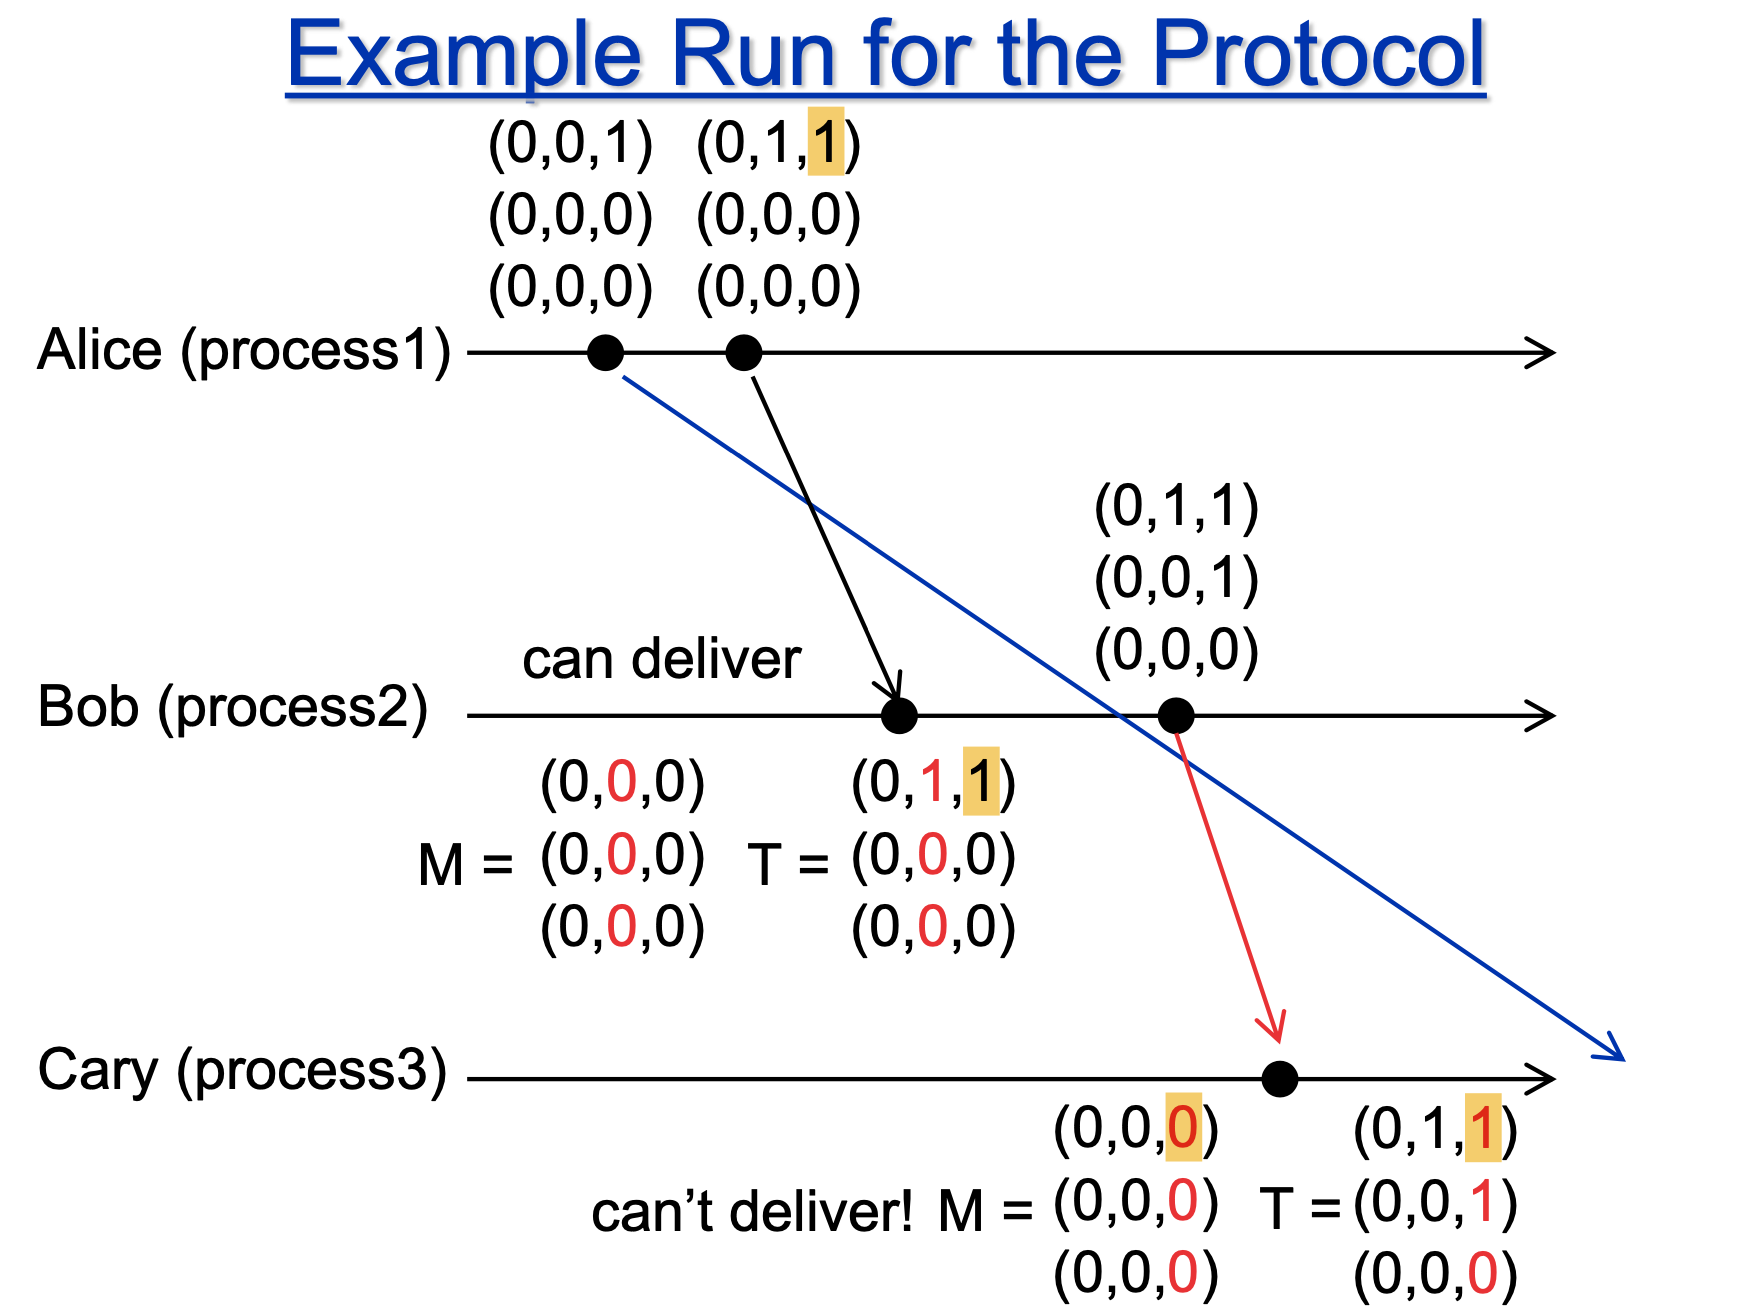
\includegraphics[width=0.7\linewidth]{cs4231-causal-ordering-protocol-example.png} 
      \end{tightcenter}
    \item $M$ never decreases!
    \item for broadcast messages, same protocol (modelled as $n$ point-to-point messages)
  \end{itemize}

  \subsection{Total Ordering of Broadcast Messages}

  \begin{itemize}
    \item \definition{broadcast} sent to all (including the sender itself)
    \item \definition{total ordering} all messages delivered to all processes in exactly the same order (aka \ildefinition{atomic broadcast})
      \begin{itemize}
        \item i.e. if every message is assigned a number, the number has to be consistent across all users
        \item total ordering only applies to broadcast messages
      \end{itemize}
    \item total ordering $\not\Rightarrow$ causal ordering
      \begin{itemize}
        \item causal ordering $\not\Rightarrow$ total ordering
      \end{itemize}
  \end{itemize}

  \subsubsection{Coordinator protocol}

  \begin{itemize}
    \item a special process is assigned as the \textbf{coordinator}
    \item to broadcast a message:
      \begin{itemize}
        \item send a message to the coordinator
        \item coordinator assigns a seq \# to the message
        \item coordinator forwards the message to all processes with the sequence number
          \begin{itemize}
            \item messages delivered according to seq\# order
          \end{itemize}
      \end{itemize}
    \item problem: coordinator has too much control
  \end{itemize}

  \subsubsection{Skeen's Algorithm}

  \begin{itemize}
    \item each process maintains
      \begin{itemize}
        \item logical clock
        \item message buffer for undelivered messages
      \end{itemize}
    \item a message in the buffer is delivered/removed if
      \begin{itemize}
        \item all messages in the buffer have been assigned numbers
        \item this message has the smallest number
      \end{itemize}
    \item protocol
      \begin{itemize}
        \item process broadcasts a message
        \item receiving processes put the message in buffer and reply (ACK) with their current logical clock value
        \item sending process picks the max clock value as message number and notifies (broadcasts) message number
      \end{itemize}
  \end{itemize}

  \begin{tightcenter}
    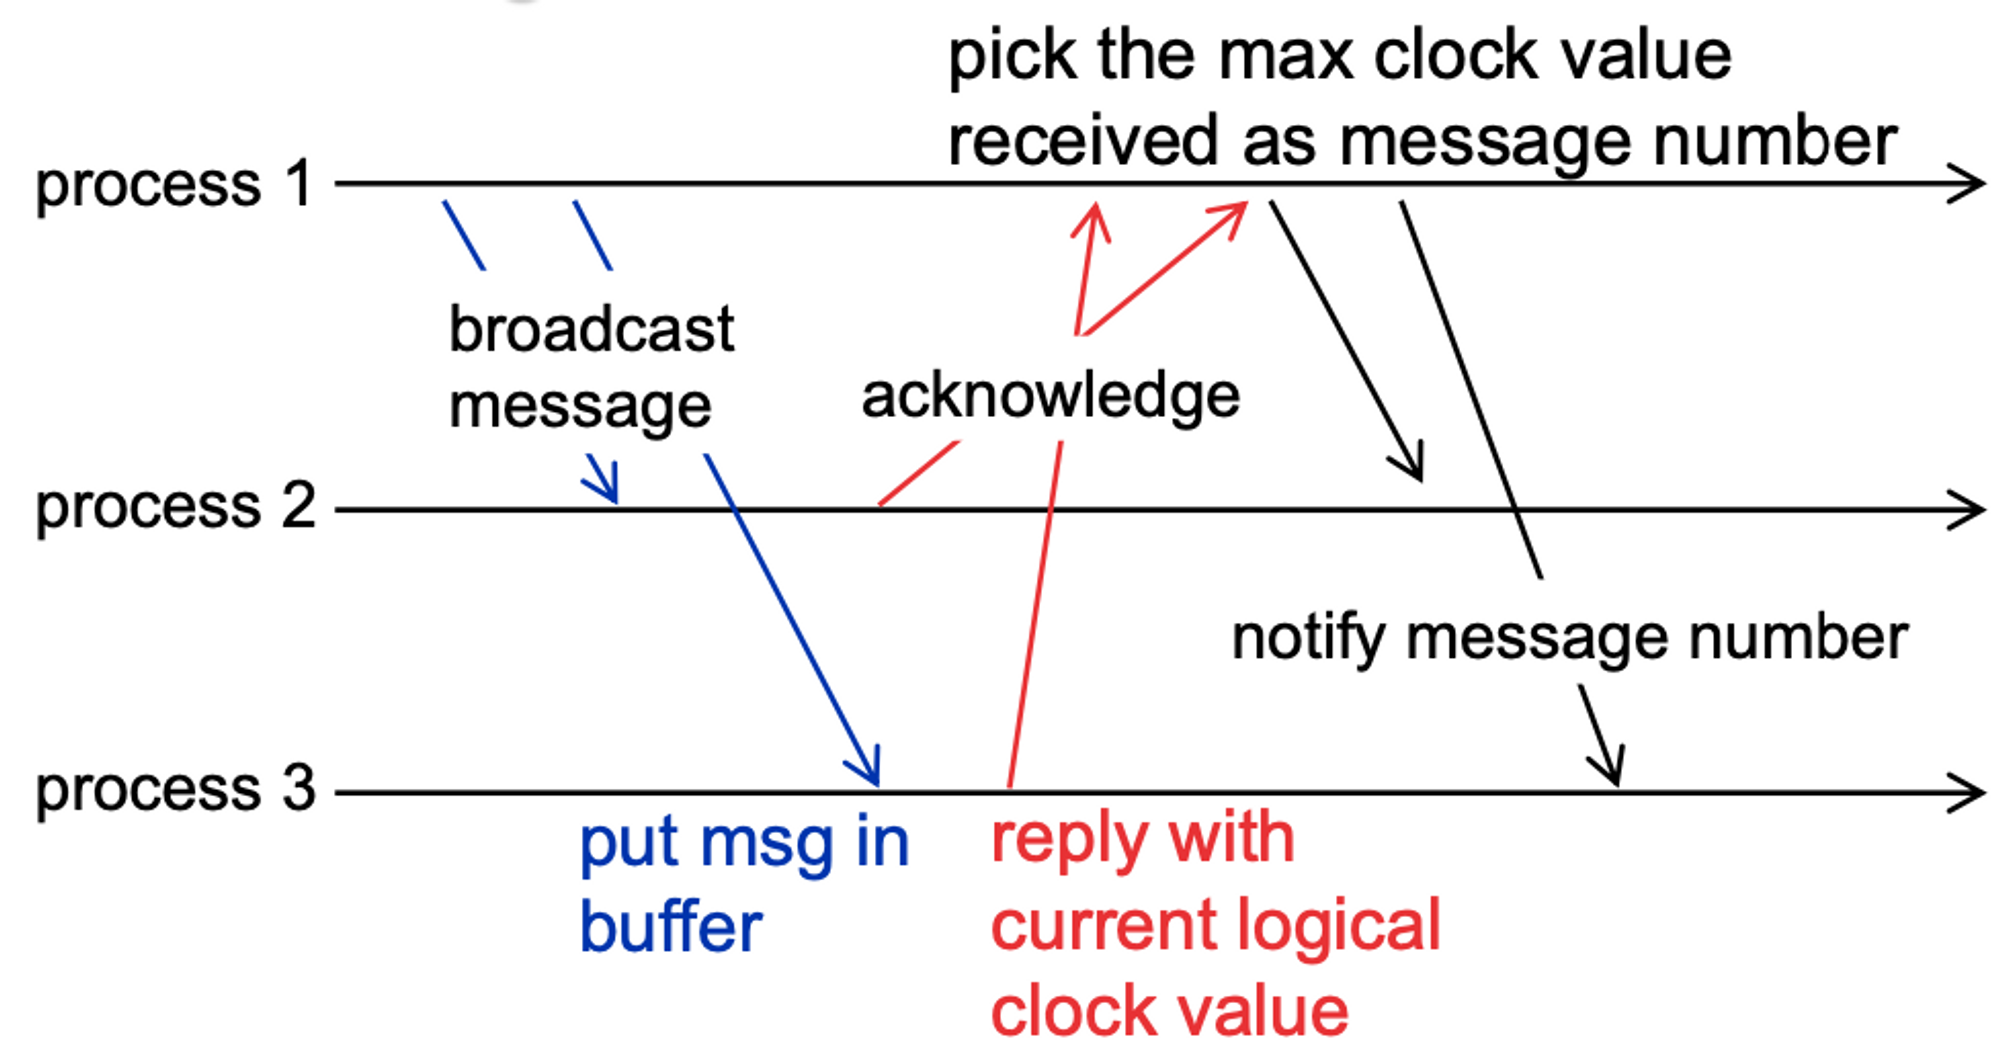
\includegraphics[width=0.7\linewidth]{cs4231-skeens-algorithm.png} 
  \end{tightcenter}

  \subsubsection{correctness proof}

  \begin{itemize}
    \item claim: all messages will be assigned message numbers
    \item claim: all messages will be delivered
    \item claim: if message $A$ has number smaller than $B$, then $B$ is delivered after $A$
      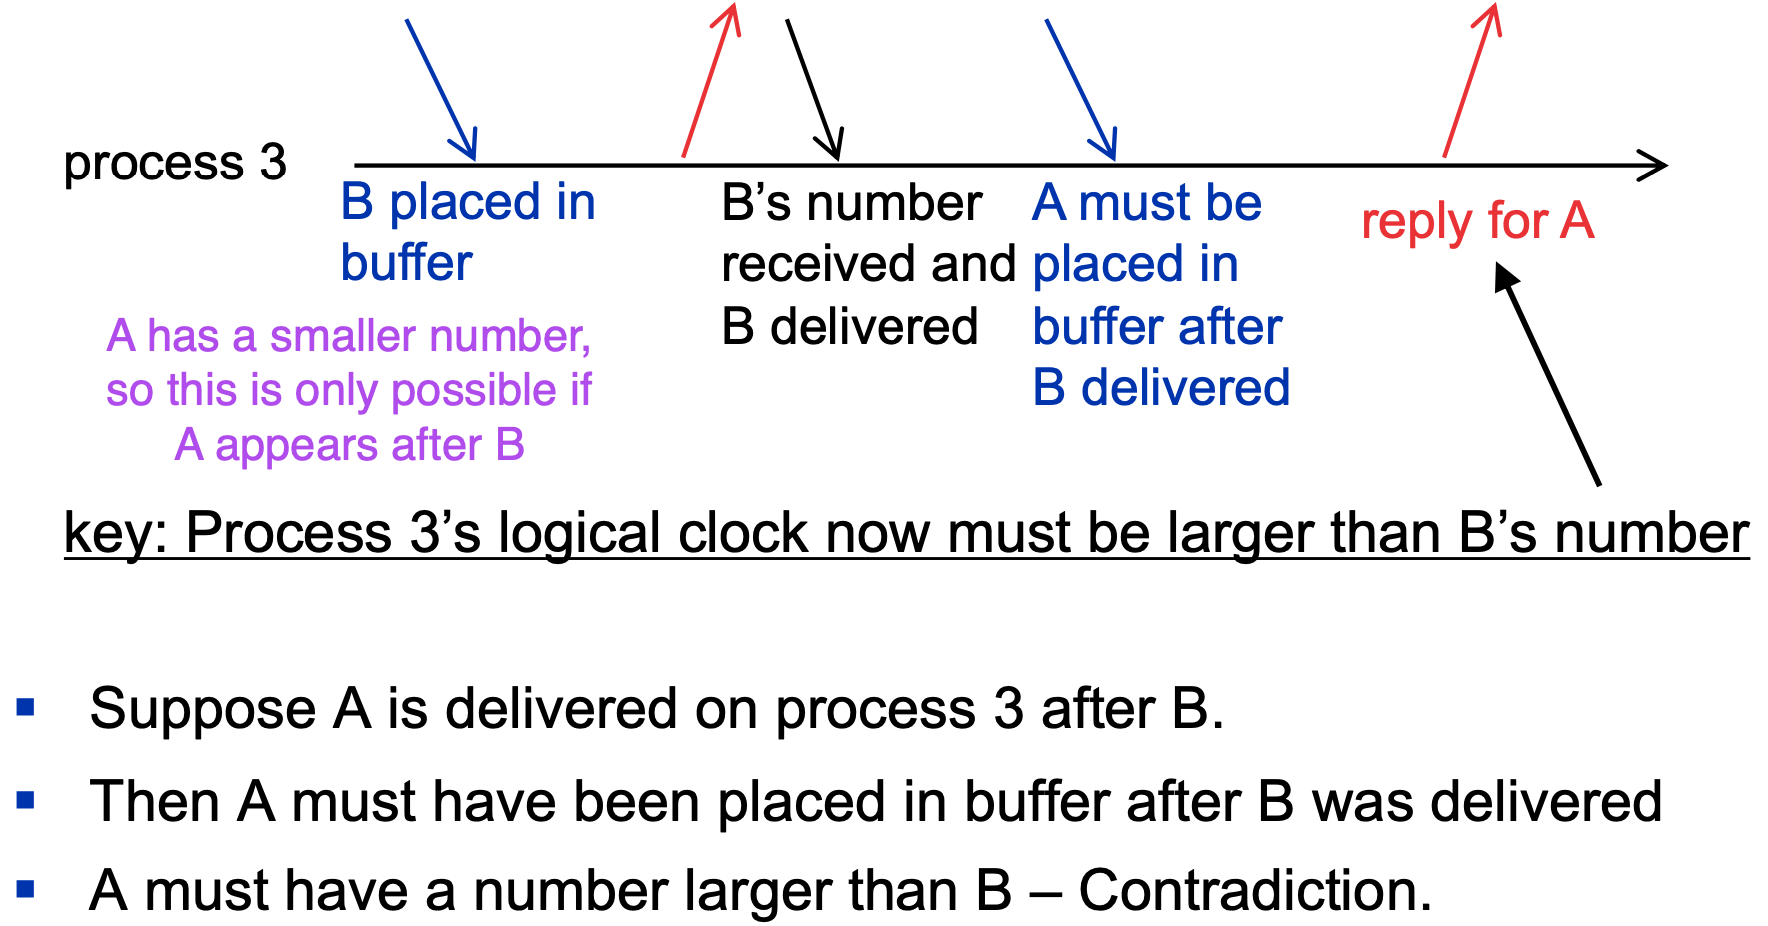
\includegraphics[width=0.7\linewidth]{cs4231-skeens-correctness-proof.png} 
  \end{itemize}

  \vfill\null
  \columnbreak

  \section{07. LEADER ELECTION}

  \begin{itemize}
    \item leader election trivially solves mutual exclusion and total order broadcast
  \end{itemize}

  \subsection{Leader Election on a Ring}

  \subsubsection{anonymous ring}

  \begin{itemize}
    \item \definition{anonymous ring} no unique identifiers
      \begin{itemize}
        \item all must run the same algorithm (otherwise the algo itself is the unique ID)
        \item node can only send messages to its neighbours
      \end{itemize}
    \item leader election impossible using deterministic algorithms
      \begin{itemize}
        \item same: initial state, state at each step, final state, algorithm on each node
      \end{itemize}
  \end{itemize}

  \subsubsection{Chang-Roberts Algorithm}

  \begin{itemize}
    \item idea: largest ID is the leader
      \begin{itemize}
        \item each node has a unique ID
        \item nodes only send messages clockwise
      \end{itemize}
  \end{itemize}

  \begin{minipage}[c]{0.77\linewidth}\color{black}
    \begin{itemize}
      \item protocol:
        \begin{itemize}
          \item node sends an election message with its own ID clockwise
          \item a node forwards an election message if the ID is larger than its own ID
            \begin{itemize}
              \item otherwise discard
            \end{itemize}
          \item a node becomes a leader if it sees its own election message
        \end{itemize}
    \end{itemize}
  \end{minipage}
  \begin{minipage}[c]{0.21\linewidth}
    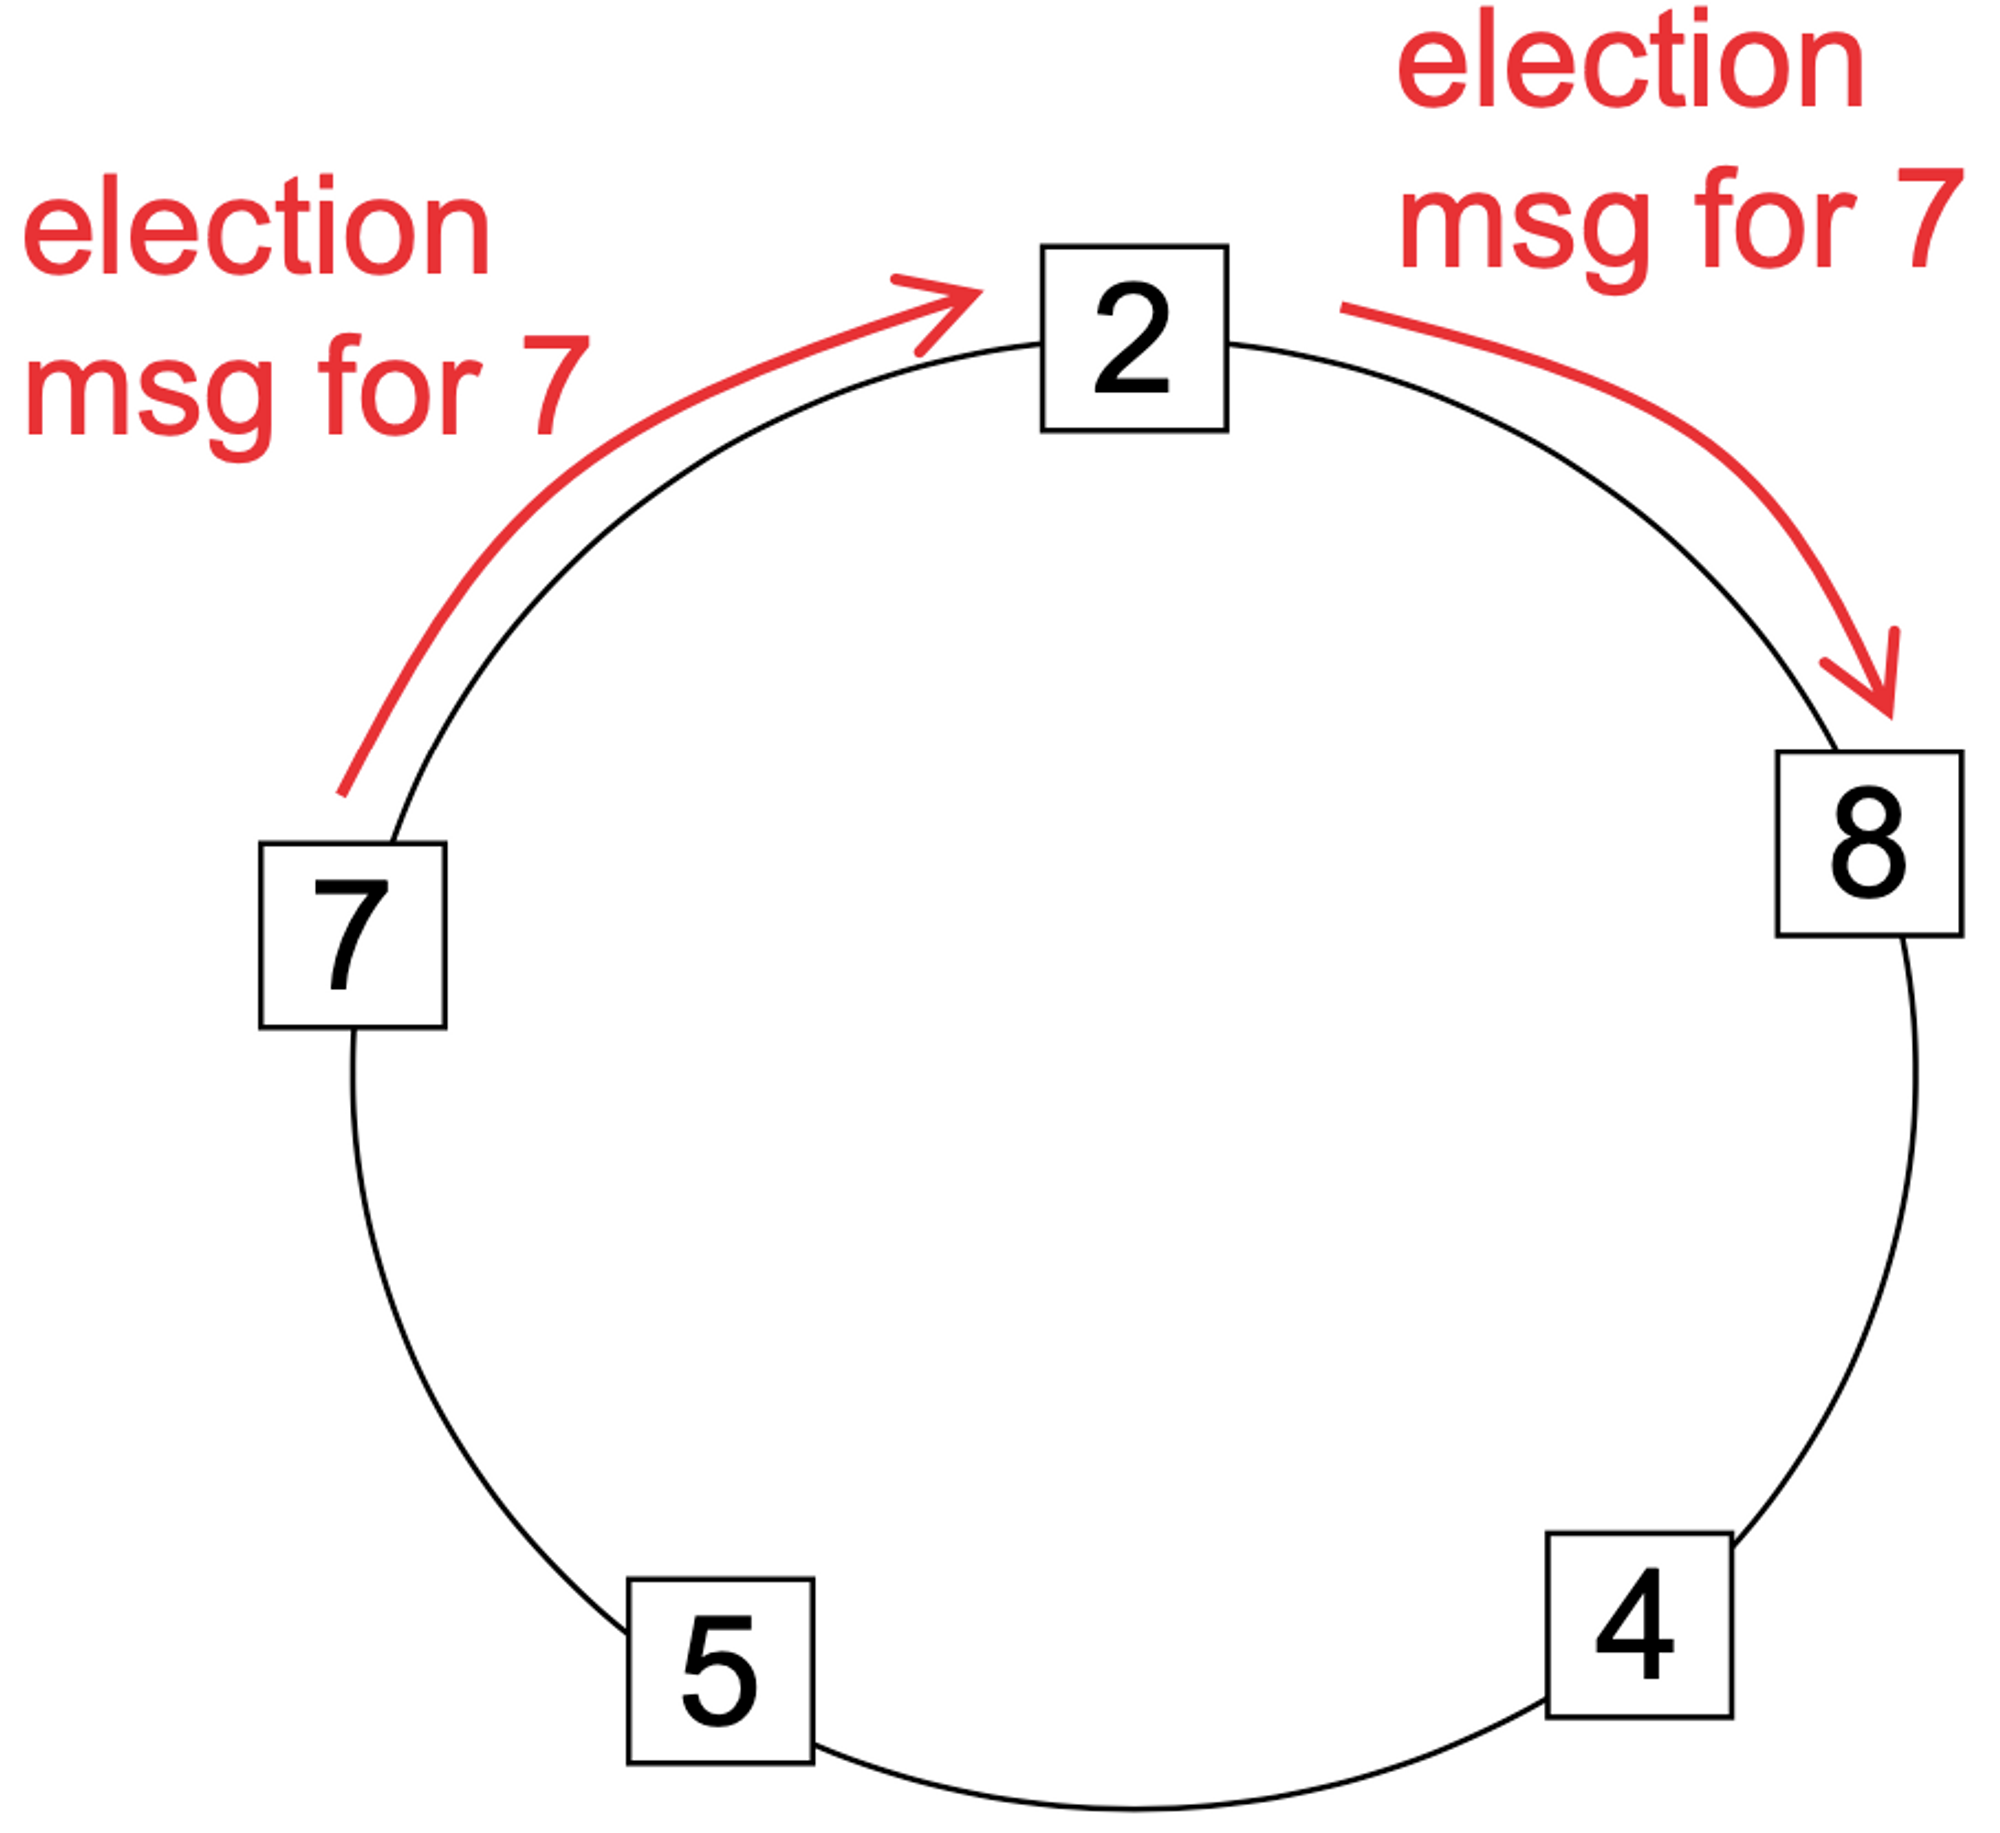
\includegraphics[width=\linewidth]{cs4231-chang-roberts.png} 
  \end{minipage}

  \begin{itemize}
    \item \textbf{performance}
      \begin{itemize}
        \item best case: $2n-1$ messages
        \item worst case: $\frac{n(n+1)}{2}$
      \end{itemize}
    \item \textbf{average case:} $O(n\log n)$
      \begin{itemize}
        \item taken over all possible orderings of nodes, each ordering having the same probability
          \begin{itemize}
            \item $(n-1)!$  total orderings of the IDs
            \item let $x_k=$ number of messages caused by node $k$'s election message
            \item we want to find $E[x_k]$ for all $k$ from 1 to n
          \end{itemize}
        \item by linearity of expectation, $E[\sum x_k] = \sum E[x_k]$
        \item $E[x_k] = \sum^k_{i=1}(i \cdot Pr[x_k=i])$
        \item $Pr[x_k=1] = Pr[\text{next node has larger ID than }k] = \frac{n-k}{n-1}$
        \item  $E[x_k] \leq E[y] = \frac{1}{p} = \frac{n-1}{n-k}$  where $y$ is a random variable denoting the number of lottery tickets we need to buy until winning the lottery (of probability $p$) for the first time
        \item $\sum^n_{k=1}E[X_k] = n + \sum^{n-1}_{k=1}E[X_k] < n +  \sum ^{n-1}_{k=1}\frac{n-1}{n-k} = n + (n-1) \sum^{n-1}_{k=1} \frac{1}{k} = n + (n-1)O(\log n) = O(n\log n)$
      \end{itemize}
  \end{itemize}

  \subsection{Leader Election on a General Graph}

  \textbf{$n$ is known}

  \begin{itemize}
    \item complete graph
      \begin{itemize}
        \item each node sends its ID to all other node
        \item wait until you receive $n$ IDs - biggest ID wins
      \end{itemize}
    \item any connected graph
      \begin{itemize}
        \item flood your ID to all other nodes
        \item ask neighbours to recursively forward ID to other neighbours
        \item wait until you receive $n$ IDs - biggest ID wins
      \end{itemize}
  \end{itemize}

  \textbf{$n$ is unknown}

  \begin{itemize}
    \item complete graph: $n$ must be known
    \item any connected graph: use an auxiliary protocol to calculate $n$
      \begin{itemize}
        \item initiated by any node that wants to know $n$
        \item establish a spanning tree starting from the initiator
      \end{itemize}
  \end{itemize}

  \subsubsection{spanning tree to calculate $n$}

  \begin{itemize}
    \item goal: each node knows its parents and children
    \item it's fine if multiple nodes initiate this process - you're just counting $n$
  \end{itemize}

  \begin{enumerate}
    \item \textbf{construct spanning tree:} initiator sends child requests
      \begin{itemize}
        \item if node has not ACKed, sends ACK and send child requests to its neighbours
        \item if node has already ACKed, reject the request
          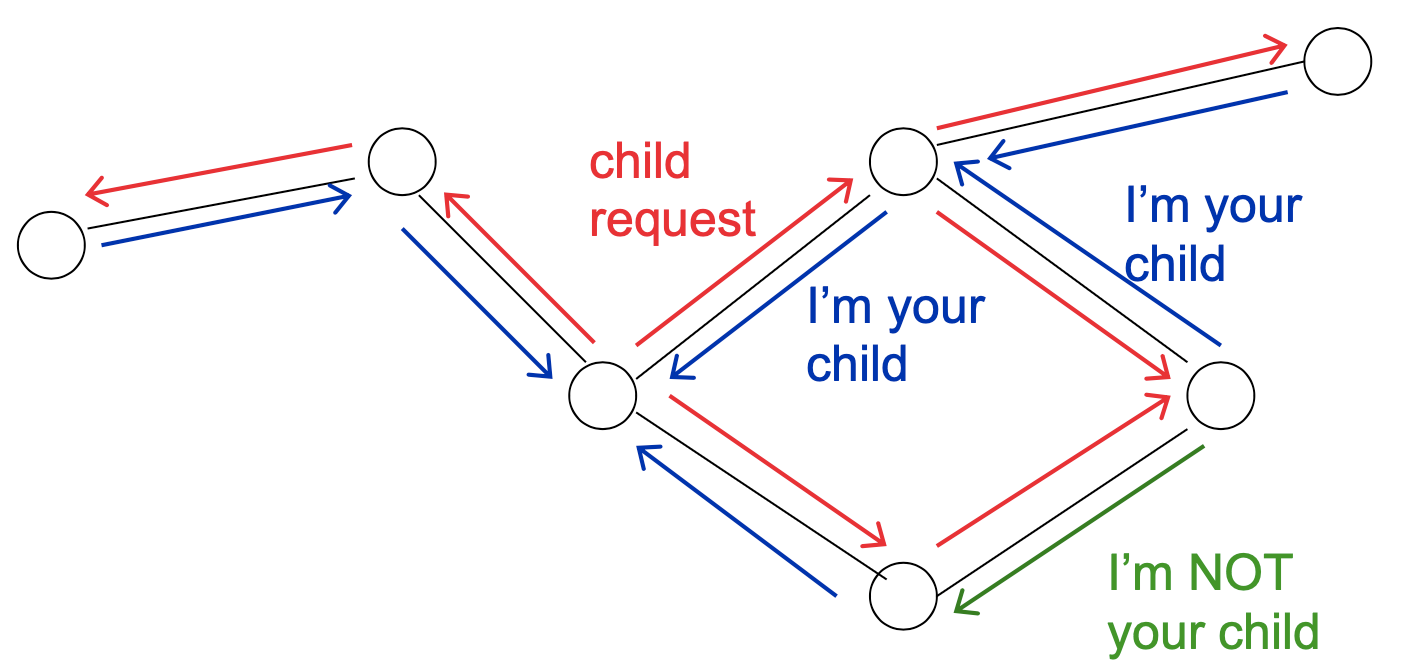
\includegraphics[width=0.5\linewidth]{cs4231-spanningtree-1.png} 
      \end{itemize}
    \item \textbf{count nodes:} initiator sends do-count request
      \begin{itemize}
        \item recursive: children will respond with 1 + the number of children they have
          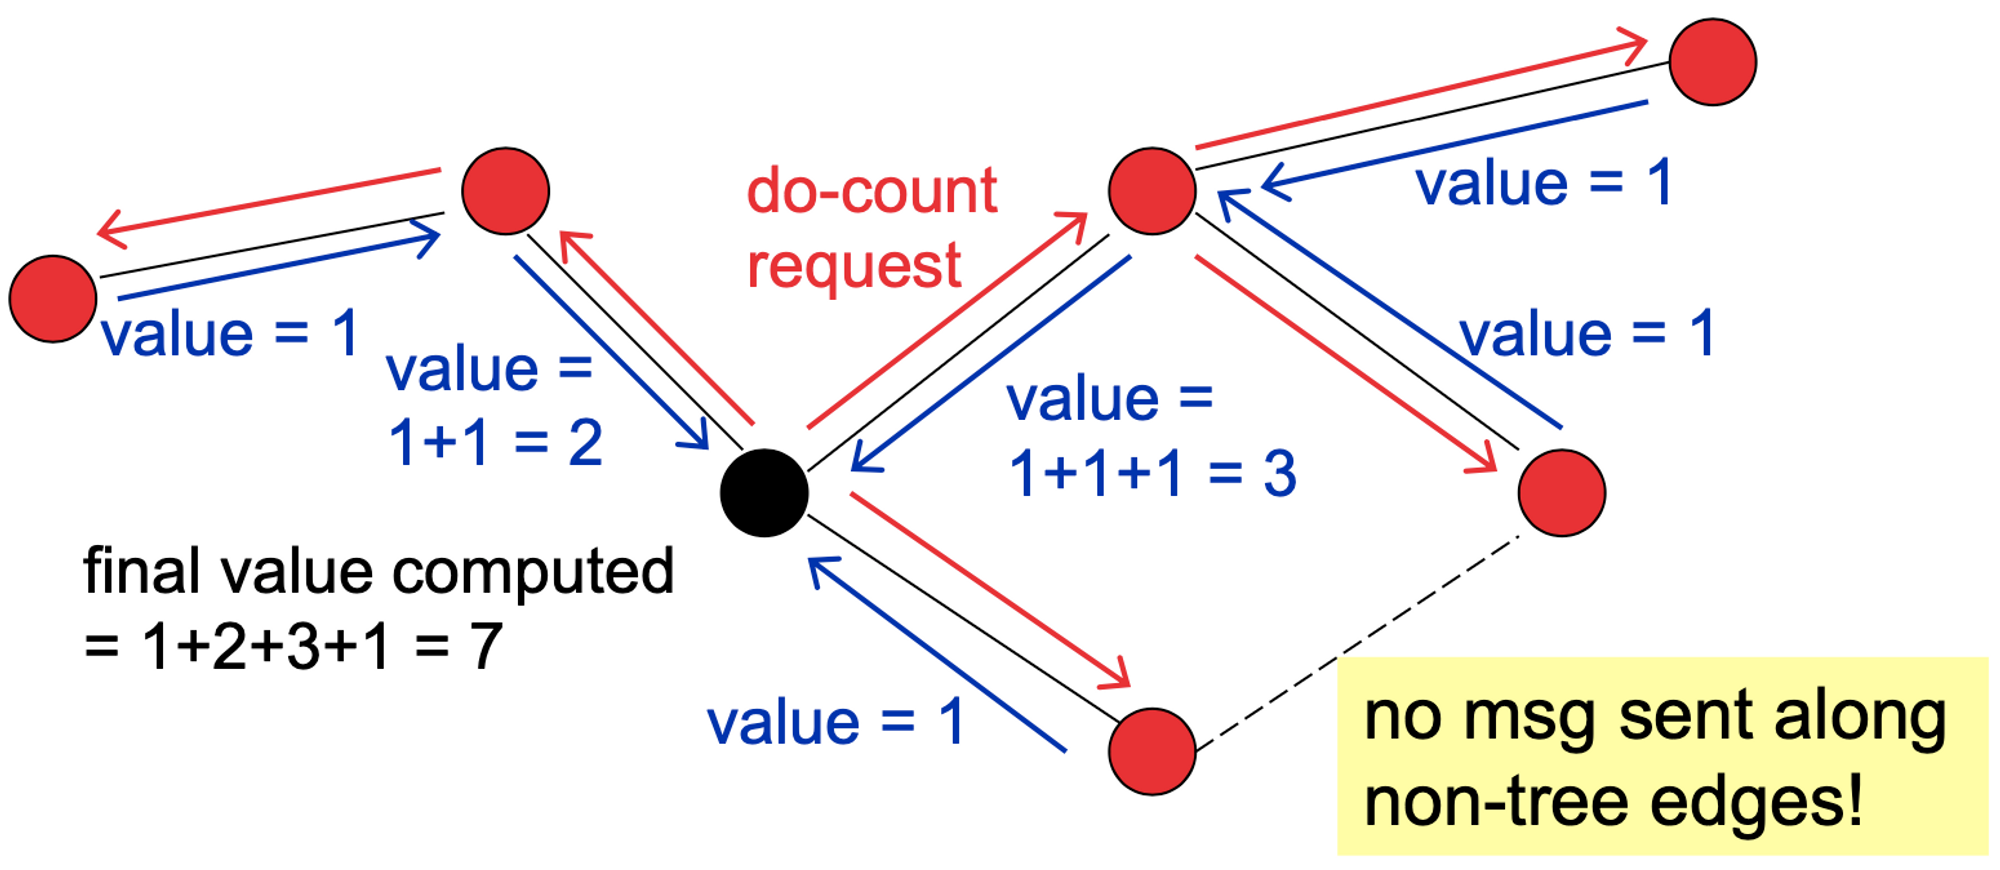
\includegraphics[width=0.6\linewidth]{cs4231-spanningtree-2.png} 
      \end{itemize}
  \end{enumerate}

  \vfill\null
  \columnbreak

  \section{08. DISTRIBUTED CONSENSUS}

  \textbf{goal}

  \begin{itemize}
    \item \definition{termination} all nodes (that have not failed) eventually decide
    \item \definition{agreement} all nodes that decide should decide on the same value
      \begin{itemize}
        \item if a node agrees then crashes, still satisfy the agreement
      \end{itemize}
    \item \definition{validity} if all nodes have the same initial input, that value should be the only possible decision value
      \begin{itemize}
        \item otherwise can decide on anything (but still satisfy Agreement)
      \end{itemize}
  \end{itemize}

  \subsection{v0. no failures}

  \begin{itemize}
    \item trivial 
  \end{itemize}

  \subsection{v1. Node crash failures}

  \textbf{model}

  \begin{itemize}
    \item failure model
      \begin{itemize}
        \item $\times$ node \ildefinition{crash failures}
          \begin{itemize}
            \item node runs the algo, but stops executing at some arbitrary point in time
          \end{itemize}
        \item $\checkmark$ communication channels are reliable
      \end{itemize}
    \item timing model
      \begin{itemize}
        \item $\checkmark$ communication channels are \ildefinition{synchronous}
          \begin{itemize}
            \item message delay has a \textit{known} upper bound $x$
            \item node processing delay has a \textit{known} upper bound $y$ (given as an input)
          \end{itemize}
      \end{itemize}
  \end{itemize}

  \subsubsection{synchronous systems and rounds}

  \begin{itemize}
    \item each round, every process:
      \begin{enumerate}
        \item does some local computation (local processing delay)
        \item sends one message to every other process (message propagation delay)
        \item receives one message from every other process
      \end{enumerate}
    \item \textbf{round duration} = clock error + msg propagation delay + local processing delay
      \begin{itemize}
        \item assume each process has a physical clock with some bounded clock error
      \end{itemize}
    \item start a new round every ROUND\_DURATION seconds
      \begin{itemize}
        \item according to local clock
      \end{itemize}
    \item each message has a round number attached to it
      \begin{itemize}
        \item a message sent in a round must be received by the end of that round on the receiver
        \item if receiver receives a message before it even starts the round: buffer the message until round starts
      \end{itemize}
  \end{itemize}

  \subsubsection{protocol}

  \begin{itemize}
    \item protocol: at each round, keep forwarding the values received
      \begin{itemize}
        \item each process sends its input to all others
        \item pick the min (or max)
      \end{itemize}
  \end{itemize}

  \begin{minipage}[c]{0.52\linewidth}\color{black}
    \begin{itemize}
      \item $f+1$ rounds needed for $f$ failures
        \begin{itemize}
          \item 1 round will be failure-free
          \item lower bound $\Omega(f)$
        \end{itemize}
      \item $f$ must be an input to the protocol
        \begin{itemize}
          \item user indicates maximum number of failures to be tolerated
        \end{itemize}
    \end{itemize}
  \end{minipage}
  \begin{minipage}[c]{0.45\linewidth}
    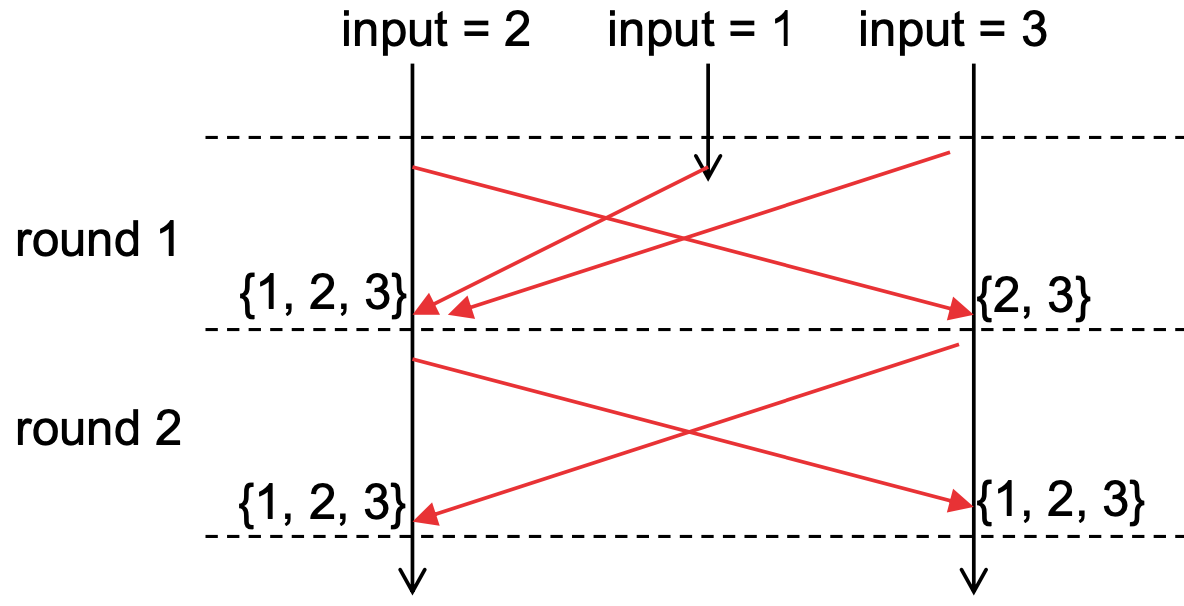
\includegraphics[width=\linewidth]{cs4231-distributedconsensus-v1.png} 
  \end{minipage}

  \subsubsection{agreement proof}

  \begin{itemize}
    \item with $f+1$ rounds and $f$ failures, there must be at least one good round
      \begin{itemize}
        \item claim: At the end of any good round $r$, all non-faulty nodes during round $r$ have the same S
        \item claim: Suppose $r$ is a good round. The value of S on any non-faulty nodes does not change during any round after $r$.
        \item claim: All nonfaulty processes at round f+1 will have the same S
      \end{itemize}
  \end{itemize}

  \subsection{v2. Link failures (Coordinated Attack)}

  \textbf{model}

  \begin{itemize}
    \item failure model
      \begin{itemize}
        \item $\checkmark$ nodes do not fail
        \item $\times$ communication channels may fail
          - drop arbitrary (unbounded) \# of msgs
      \end{itemize}
    \item timing model
      \begin{itemize}
        \item $\checkmark$ synchronous
      \end{itemize}
    \item goal: termination/agreement/validity
      \begin{itemize}
        \item impossible to achieve these using a deterministic algorithm
          \begin{itemize}
            \item cos communication channel can drop all messages
            \item execution $\alpha$ is \definition[from execution $\beta$]{indistinguishable} if the node sees the same messages and inputs in both execution
              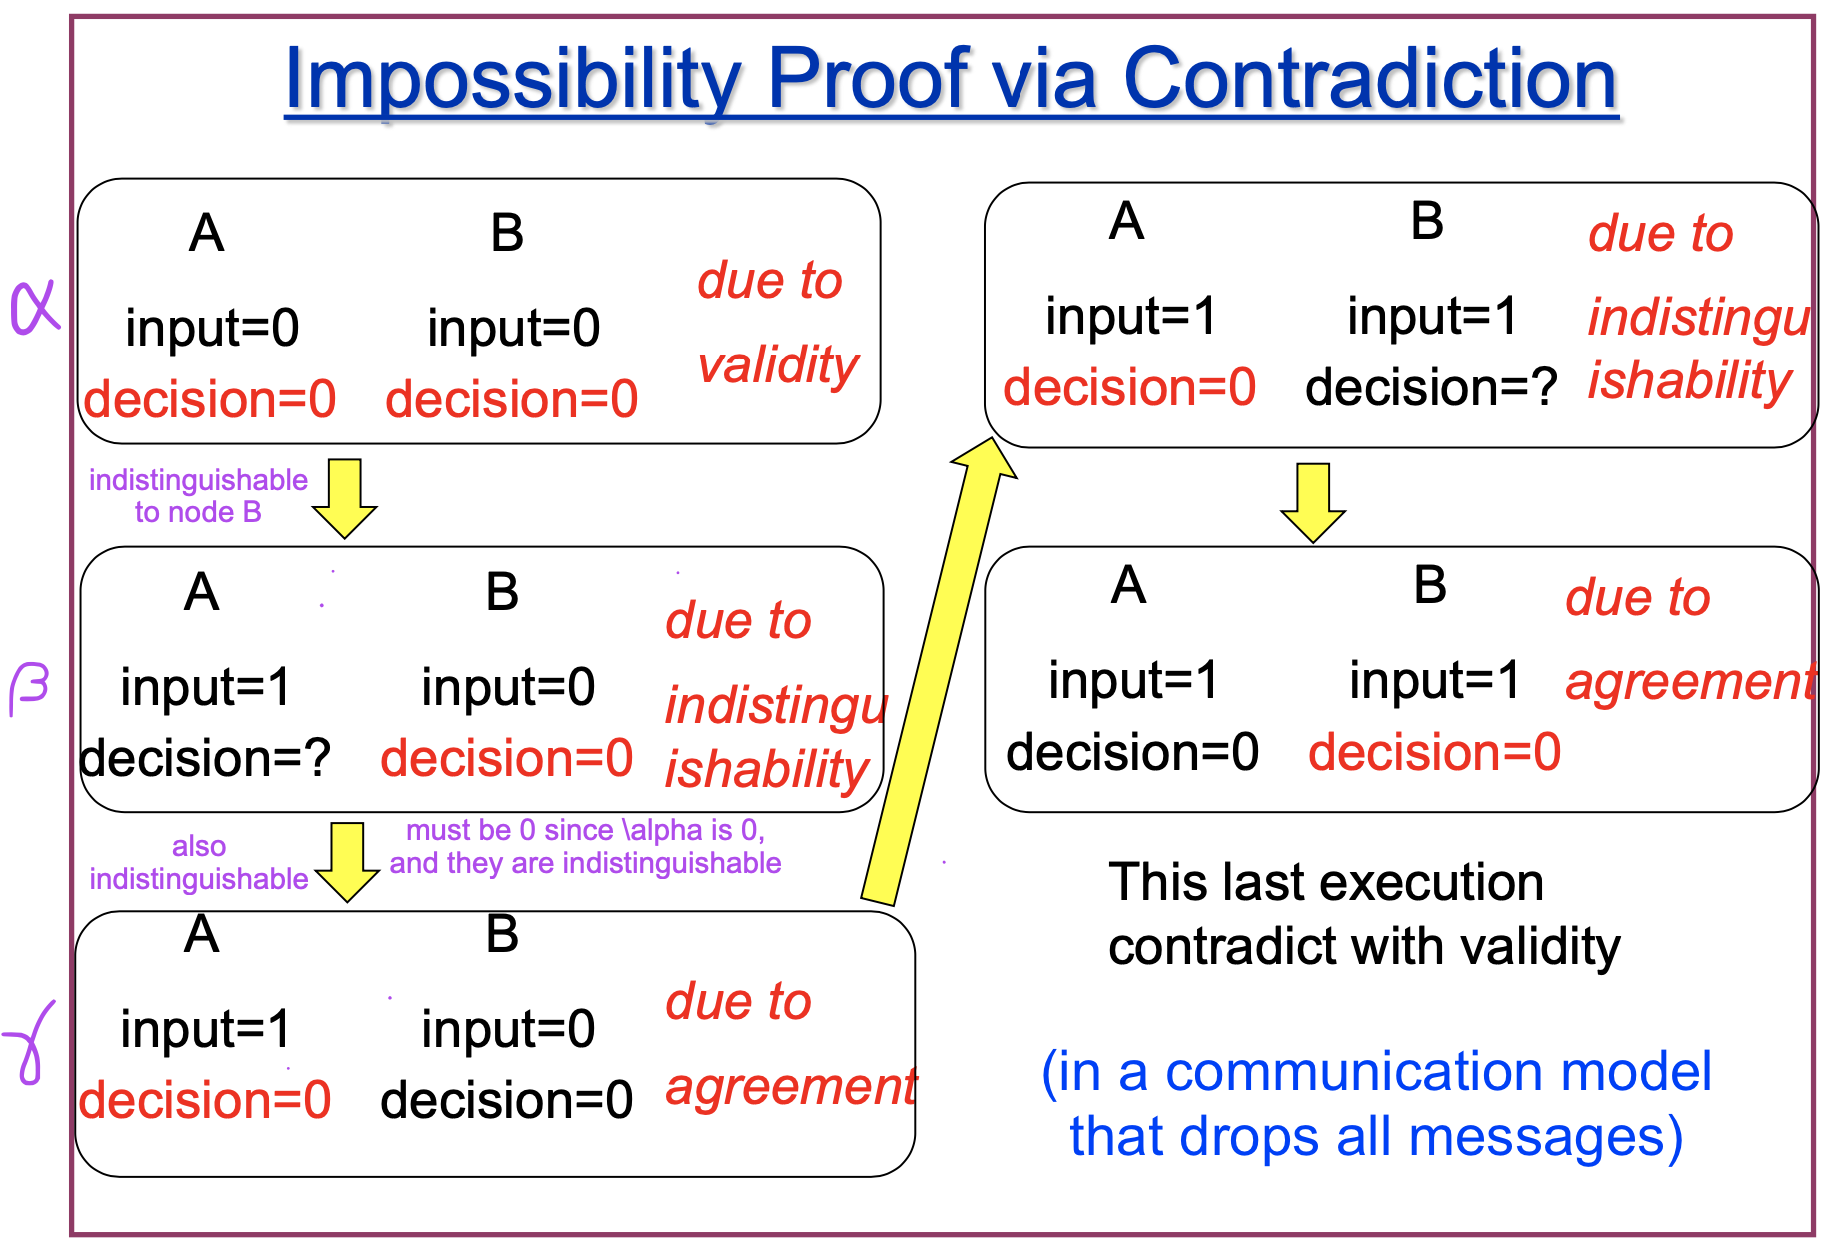
\includegraphics[width=0.8\linewidth]{cs4231-distributedconsensus-v2-impossibility.png} 
          \end{itemize}
      \end{itemize}
  \end{itemize}

  \begin{minipage}[c]{0.5\linewidth}\color{black}
    \textbf{v2.1. Weakened goal}

    still impossible using deterministic algo

    \begin{itemize}
      \item if all nodes start with 0, the decision = 0
      \item if all nodes start with 1 and no message is lost during execution, decision = 1
      \item otherwise, any consensus
    \end{itemize}
  \end{minipage}
  \begin{minipage}[c]{0.48\linewidth}
    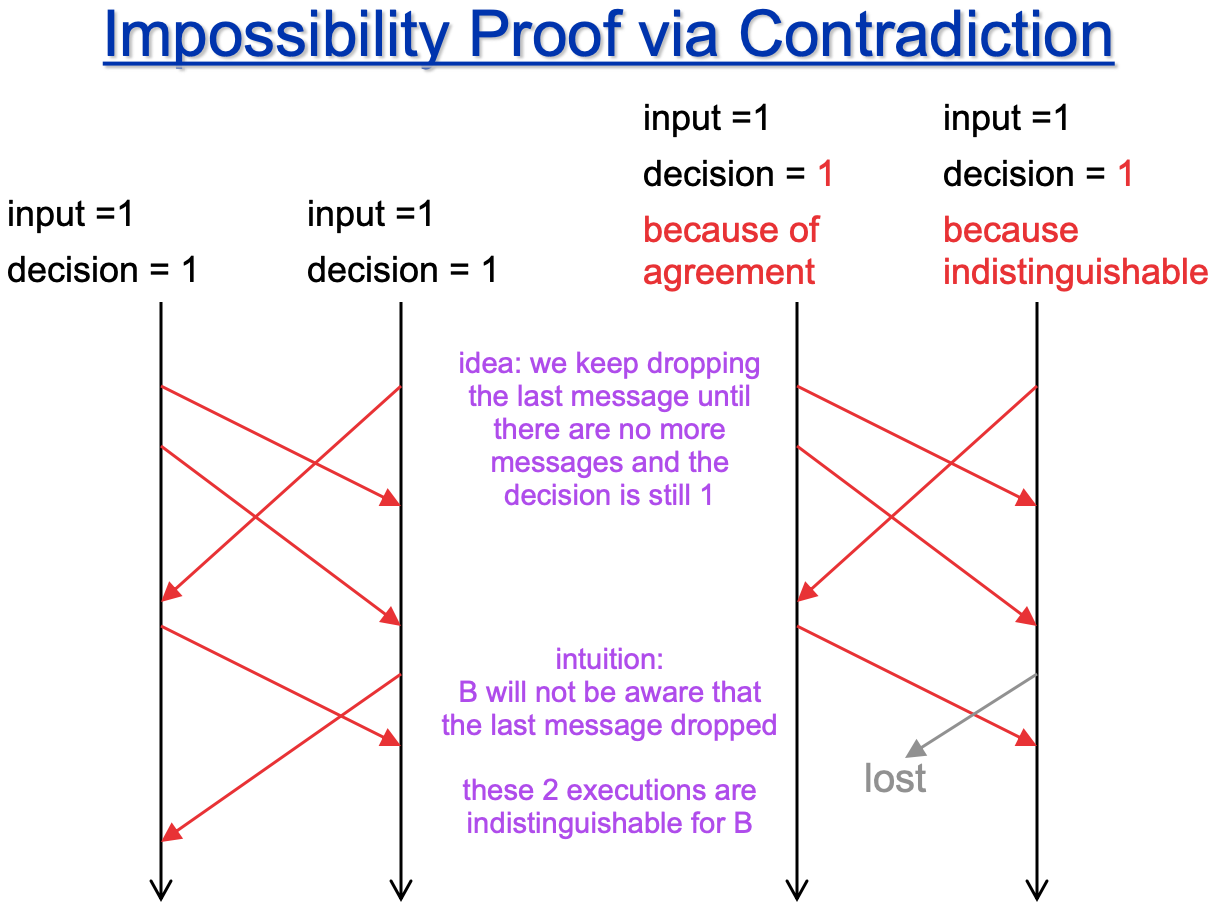
\includegraphics[width=\linewidth]{cs4231-distributedconsensus-v2-1-impossibility.png} 
  \end{minipage}

  \subsection{v2.2. Limited disagreement (small error)}

  \begin{itemize}
    \item \textbf{goal}
      \begin{itemize}
        \item termination
        \item \textit{agreement:} all nodes decide on the same value with probability $1-\epsilon$
        \item \textit{validity}
          \begin{itemize}
            \item if all nodes start with 0, decision = 0
            \item if all nodes start with 1 and no message is lost throughout, decision = 1
            \item else: anything
          \end{itemize}
      \end{itemize}
    \item \textbf{adversary} maximises error probability
      \begin{itemize}
        \item $\checkmark$ set inputs of the processes
        \item $\checkmark$ cause message losses
        \item $\times$ does not know the outcome of any randomisation
      \end{itemize}
  \end{itemize}

  \subsubsection{randomised algorithm}

  \begin{itemize}
    \item 2 processes (P1, P2), predetermined number ($r$) of rounds
      \begin{itemize}
        \item adversary determines which messages are lost \textit{before seeing random choices}
      \end{itemize}
  \end{itemize}

  \begin{minipage}[c]{0.73\linewidth}\color{black}
    \begin{itemize}
      \item protocol
        \begin{itemize}
          \item P1 picks a random integer $bar \in [1..r]$
          \item each P1, P2 maintains a $level$ variable L1, L2
            \begin{itemize}
              \item L1 and L2 differ by at most 1
            \end{itemize}
          \item each round: send each other messages
            \begin{itemize}
              \item attach input, $bar$ and $level$ to each message
              \item P1: set L1 = L2+1
                \begin{itemize}
                  \item (symmetric) same for P2
                \end{itemize}
            \end{itemize}
          \item \attention L1/L2 never decreases!
        \end{itemize}
    \end{itemize}
  \end{minipage}
  \begin{minipage}[c]{0.24\linewidth}
    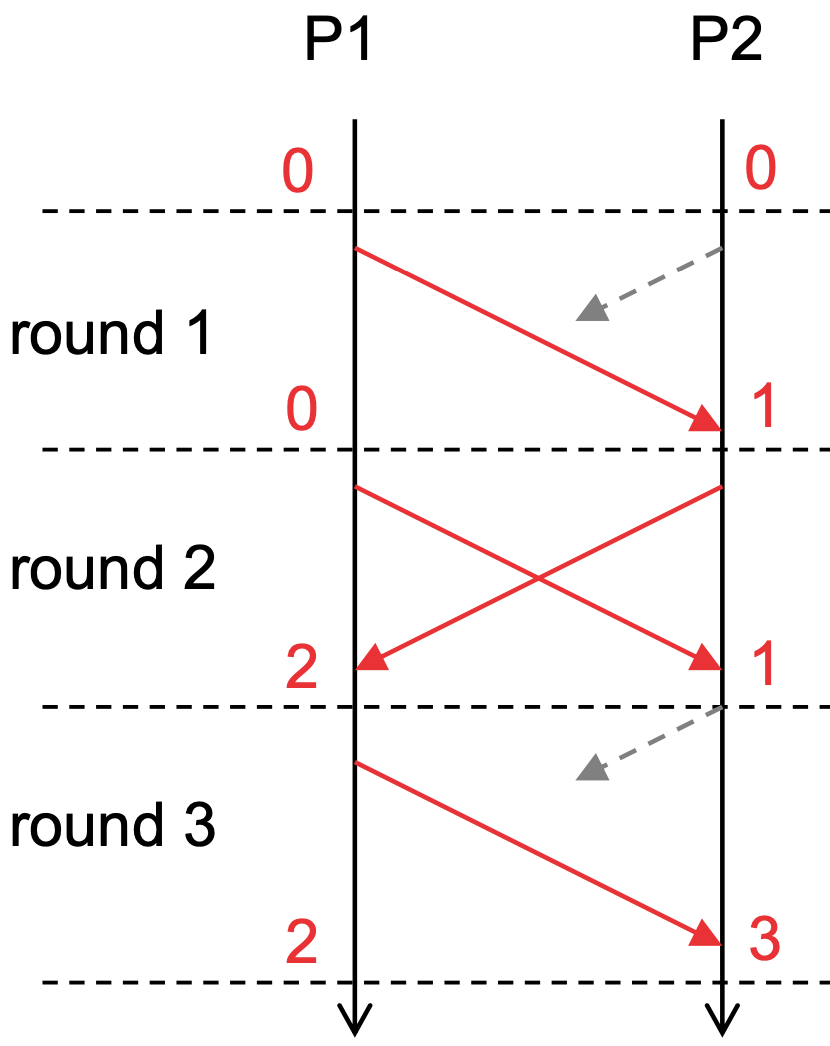
\includegraphics[width=\linewidth]{cs4231-distributedconsensus-level-algo.png} 
  \end{minipage}

  \begin{itemize}
    \item decision rule: after $r$ rounds, P1/P2 decide on 1 $\iff$
      \begin{itemize}
        \item it knows its input \textit{and} the other process input are both 1
        \item it knows bar (always true for P1)
        \item its $level \geq bar$
      \end{itemize}
    \item error probability $\epsilon = \frac{1}{r}$
  \end{itemize}

  \begin{tightcenter}
    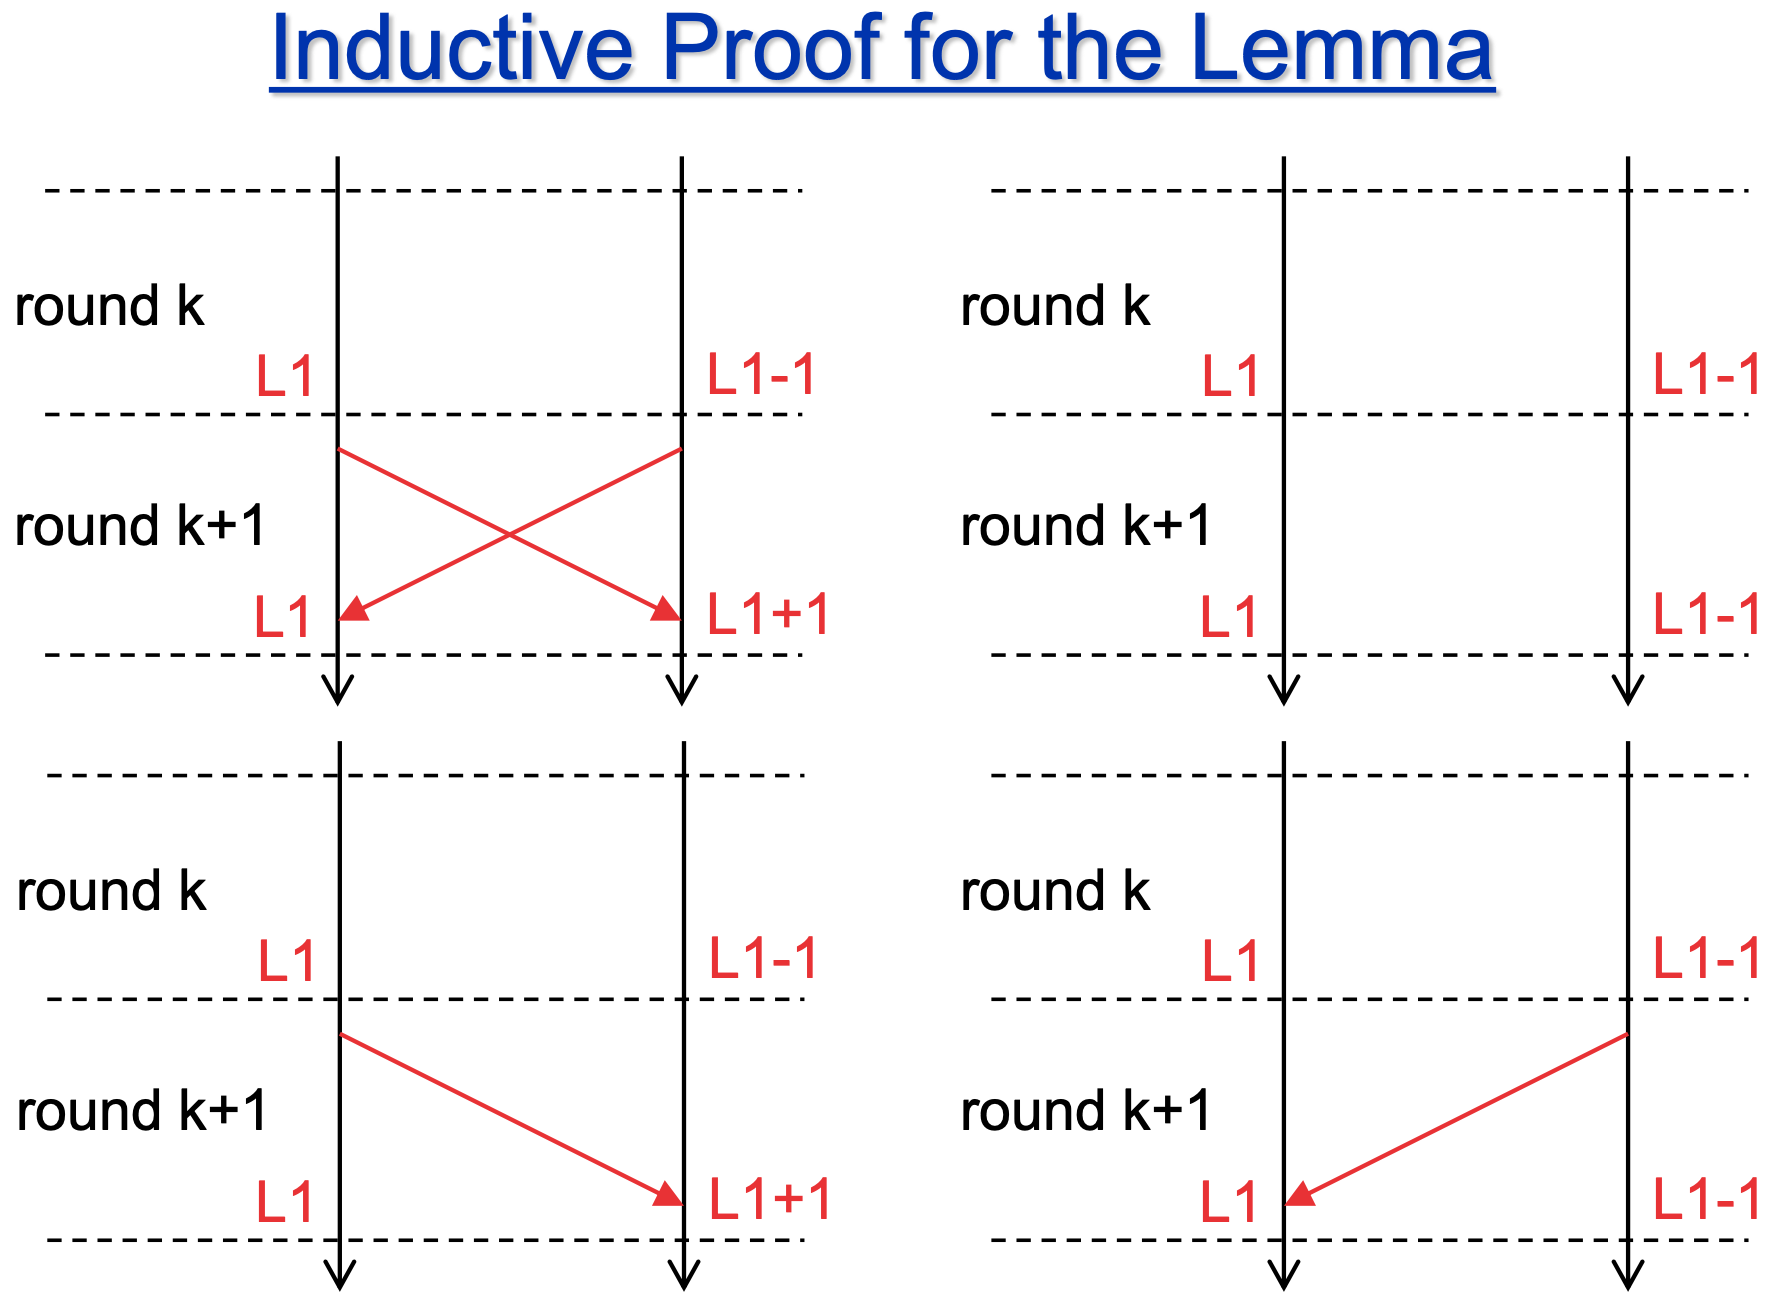
\includegraphics[width=0.45\linewidth]{cs4231-distributedconsensus-level-induction.png} 
    \includegraphics[width=0.53\linewidth]{cs4231-distributedconsensus-level-error.png} 
  \end{tightcenter}

  \subsection{v3. Node crash failures + Asynchronous}

  \textbf{model}

  \begin{itemize}
    \item failure model
      \begin{itemize}
        \item $\checkmark$ reliable channel
        \item $\times$ node crash failures
      \end{itemize}
    \item timing model
      \begin{itemize}
        \item \definition{asynchronous} process delay and message delay are \textit{finite but unbounded}
        \item can no longer define a round
      \end{itemize}
    \item goal: termination/agreement/validity
    \item \definition[(Fischer, Lynch, Paterson)]{FLP theorem} the distributed consensus problem under asynchronous communication model is impossible to solve even with a single node crash failure
      \begin{itemize}
        \item fundamentally, because the protocol cannot accurately detect node failure
      \end{itemize}
  \end{itemize}

  \subsubsection{formalisms of FLP theorem}

  \begin{itemize}
    \item global state of a system = all process states + message system state
      \begin{itemize}
        \item message system captures on-the-fly messages: $\{(p, m) \vert \text{message $m$ on the fly to process $p$}\}$
        \item all messages are distinct
        \item sending and receiving operations are adding and removing content from the message system, and changing process local state
      \end{itemize}
    \item each step given a global state is fully described by p’s receiving m
      \begin{itemize}
        \item $(p, m)$ is an event
          \begin{itemize}
            \item events are inputs to the state machine, that cause state transitions
          \end{itemize}
        \item event $e$ can be applied to the global state G if either $m==null$ or $(p, m)$ is in the message system
      \end{itemize}
    \item execution of any protocol is an \textit{infinite sequence of events}
      \begin{itemize}
        \item process fail = \textit{finite} number of steps
      \end{itemize}
    \item schedule $\sigma$ is a sequence of events that captures the execution of a protocol
      \begin{itemize}
        \item $G'=\sigma(G)$ means we apply $\sigma$ to G to get G’
        \item must make sure $\sigma$ can be applied to G (aka G’ is \ildefinition{reachable} from G if $\exists \sigma$ such that $G'=\sigma(G)$)
      \end{itemize}
    \item messages have unbounded but finite delay - every message is eventually delivered
  \end{itemize}

  \subsection{v4. Node Byzantine failures}

  \textbf{model}

  \begin{itemize}
    \item failure model
      \begin{itemize}
        \item $\checkmark$ reliable channels
        \item $\times$ \definition{byzantine failures} nodes can behave unexpectedly and arbitrarily
          \begin{itemize}
            \item must consider the worst case where nodes intentionally break the protocol
          \end{itemize}
      \end{itemize}
    \item timing model
      \begin{itemize}
        \item $\checkmark$ synchronous
      \end{itemize}
    \item goal: termination/agreement/validity for \textit{non-faulty nodes} only
      \begin{itemize}
        \item \textit{agreement:} bad nodes can't be forced to decide
        \item \textit{validity:} if all the good nodes have the same initial input, that value should be the only possible decision value 
      \end{itemize}
    \item \textbf{byzantine consensus threshold} for $n$ processes, $f$ possible byzantine failures
      \begin{itemize}
        \item if $n \leq 3f$, then the byzantine consensus problem cannot be solved
      \end{itemize}
  \end{itemize}

  \subsubsection{protocol for $n \geq 4f+1$}

  \begin{itemize}
    \item intuition
      \begin{itemize}
        \item \textit{rotating coordinator:} process $i$ is the coordinator for phase $i$
        \item coordinator sends a proposal to all processes
        \item a phase is a \ildefinition{deciding phase} if the coordinator is nonfaulty
          \begin{itemize}
            \item agreement after a phase with a good coordinator
            \item if the coordinator is non faulty, all processes see the proposal
          \end{itemize}
      \end{itemize}
    \item protocol
      \begin{itemize}
        \item $f+1$ phases (cos at most $f$ bad nodes)
          \begin{itemize}
            \item each phase is 2 rounds
          \end{itemize}
        \item set local value = input
        \item each phase
          \begin{itemize}
            \item round 1: all-to-all broadcast
              \begin{itemize}
                \item send your local value to all processes
              \end{itemize}
            \item round 2: coordinator round
              \begin{itemize}
                \item set proposal to majority ($>n/2$)
                \item send the proposal to everyone
              \end{itemize}
            \item decide whether to listen to the coordinator
              \begin{itemize}
                \item if overwhelming majority ($> \frac{n}{2}+f$), set local value to majority
                \item else, set local value = coordinator’s proposal
              \end{itemize}
          \end{itemize}
      \end{itemize}
  \end{itemize}

  \textbf{proof}

  \begin{itemize}
    \item Lemma 1: if all good processes have the same local value at the beginning of a given phase, then this remains true at the end of a phase
      \begin{itemize}
        \item since we have $n-f$ good processes and $n-f > \frac{n}{2} + f$, they will be the overwhelming majority
      \end{itemize}
    \item Lemma 2: if the coordinator in a phase is good, agreement will be achieved at the end of that phase
      \begin{itemize}
        \item case 1: coordinator sees (and proposes) a majority=$x$
          \begin{itemize}
            \item then $x$ appears (>n/2) times, of which >n/2-f must be from good processes
            \item thus other processes will see $x$ (>n/2-f) times
            \item so no other value can be overwhelming majority
          \end{itemize}
        \item case 2: coordinator receives equal distribution
          \begin{itemize}
            \item then it’s impossible for anyone to see an overwhelming majority
            \item for coordinator, no value $x$ appears (>n/2) times
            \item thus for other processes, impossible for any $y \neq x$ to appear (>n/2+f) times
          \end{itemize}
      \end{itemize}
    \item \textit{termination:} after f+1 phases
    \item \textit{validity:} follows from lemma 1
    \item \textit{agreement:}
      \begin{itemize}
        \item with f+1 phases, at least one is a deciding phase
        \item by Lemma 2, all good processes will agree at deciding phase
        \item by Lemma 1, after a deciding phase, additional phases will not disrupt the agreement achieved
      \end{itemize}
  \end{itemize}

  \begin{tightcenter}
    \includegraphics[width=0.65\linewidth]{cs4231-distributedconsensus-summary.png} 
  \end{tightcenter}

  \vfill\null
  \columnbreak

  \section{10. SELF-STABILISATION}

  \begin{itemize}
    \item state of a distributed system is either legal or illegal
      \begin{itemize}
        \item based on application semantics
      \end{itemize}
    \item \definition{self-stabilising} if
      \begin{itemize}
        \item starting from any (legal or illegal) state, the protocol will eventually reach a legal state if there are no more faults
        \item once in a legal state, it will only transit to a legal state unless there are faults
      \end{itemize}
    \item typically runs in the background and never stops
  \end{itemize}

  \subsection{Rotating Privilege Problem}

  \begin{itemize}
    \item a ring of $n$ processes
      \begin{itemize}
        \item each process can only communicate with neighbours
      \end{itemize}
    \item at any time, only one node may have the privilege
    \item privilege is like a token
  \end{itemize}

  \subsubsection{algorithm}

  \begin{itemize}
    \item each process $i$ has local integer variable $V_i\quad$ where $0 \leq V_i \leq k, \quad k\geq n$
    \item one red process and some blue processes (allocate before running the algorithm)
  \end{itemize}

  \begin{minipage}[c]{0.57\linewidth}\color{black}
    \begin{itemize}
      \item \textcolor{red}{red} process
        \begin{itemize}
          \item retrieve value $L$ of clockwise neighbour
          \item if $V==L$: (has privilege)
            \begin{itemize}
              \item increment $V$\texttt{++} with mod $k$
            \end{itemize}
        \end{itemize}
      \item \textcolor{blue}{blue} process
        \begin{itemize}
          \item retrieve value $L$ of clockwise neighbour
          \item if $V\neq L$: (has privilege)
            \begin{itemize}
              \item set $V=L$
            \end{itemize}
        \end{itemize}
    \end{itemize}
  \end{minipage}
  \begin{minipage}[c]{0.4\linewidth}
    \includegraphics[width=\linewidth]{cs4231-rotating-privilege-example.png} 
  \end{minipage}

  \subsubsection{legal states}

  \begin{itemize}
    \item Lemma: there are only 2 legal states
      \begin{enumerate}
        \item all $n$ values same $\quad\Rightarrow$ red process privilege
        \item only 2 different values forming 2 consecutive bands, with one band starting from the red process $\quad\Rightarrow$ blue process privilege
      \end{enumerate}
  \end{itemize}

  \subsection{Self-Stabilising Spanning Tree}

  \begin{itemize}
    \item given $n$ processes connected by an undirected graph and one special process P1, construct a spanning tree rooted at P1
    \item each process maintains 2 variables: \textbf{parent} and \textbf{dist} (to root, $\geq 0$)
      \begin{itemize}
        \item faults: wrong value of these variables
      \end{itemize}
  \end{itemize}

  \subsubsection{algorithm}

  \begin{itemize}
    \item P1 repeatedly executes `dist=0; parent=null;`
    \item all other nodes periodically execute
      \begin{itemize}
        \item retrieve dist from all neighbours
          \begin{itemize}
            \item set own $dist = 1 + \min($neighbour dists$)$
          \end{itemize}
        \item set own parent = neighbour with smallest dist
          \begin{itemize}
            \item break tie: based on ID (e.g. smaller ID)
          \end{itemize}
      \end{itemize}
  \end{itemize}

  \subsubsection{proof}

  \begin{itemize}
    \item \definition{phase} minimum time period where each process has executed its code at least once (can be more than once)
    \item assume that the topology doesn’t change
      \begin{itemize}
        \item i.e. no additional faults - we only need to reason about self-stabilising algos if there are no additional faults
      \end{itemize}
    \item let
      \begin{itemize}
        \item $A_i$ be the \ildefinition{level} of process $i$ (length of the shortest path from $i$ to root)
          \begin{itemize}
            \item $A_i$ will not change
          \end{itemize}
        \item $dist_i$ be the value of dist on $i$
          \begin{itemize}
            \item $dist_i$ may change
          \end{itemize}
      \end{itemize}
    \item properties of levels of the nodes
      \begin{enumerate}
        \item a node at level $X$ has at least one neighbour in level $X-1$
          \begin{itemize}
            \item if there is a neighbour with level $<X-1$, then the node can have a smaller level $<X$
          \end{itemize}
        \item a node at level $X$can only have neighbours in level $X-1,X,X+1$
          \begin{itemize}
            \item for X-1: same proof as (1)
            \item if there is a neighbour with >X+1, then that node can be X+1 by going through the node instead
          \end{itemize}
      \end{enumerate}
    \item lemma: at the end of phase $r$,
      \begin{enumerate}
        \item any process $i$ whose $A_i \leq r-1$, has $dist_i = A_i$
          \begin{itemize}
            \item if level is < r, the distance value must become correct (i.e. dist=level)
          \end{itemize}
        \item any process $i$ whose $A_i \geq r$, has $dist_i \geq r$
          \begin{itemize}
            \item for the remaining processes, the distance value is $\geq r$ and may still be incorrect
          \end{itemize}
      \end{enumerate}
    \item \textbf{proof:} by induction
      \begin{itemize}
        \item base: holds for $r=1$ 
        \item assume lemma holds at phase $r$ and consider phase $r+1$
      \end{itemize}
  \end{itemize}

  \subsubsection{common self-stabilisation proof technique}

  \begin{itemize}
    \item Step 1: Prove that the $t$ actions will not roll back what is already achieved so far by phase r (no backward move)
    \item Step 2: Prove that at some point, each node will achieve more (forward move)
    \item Step 3: Prove that the $t$ actions will not roll back the effects of the forward move after the forward move happens (no backward move after the forward move)
  \end{itemize}

\end{multicols*}

\end{document}
